
\newpage
%+++++++++++++++++++++++++++++++
%+++++++++++++++++++++++++++++++
\mysubsection{Nodes}

%+++++++++++++++++++++++++++++++++++
\mysubsubsection{NodePoint}
A 3D point node for point masses or solid finite elements which has 3 displacement degrees of freedom for second order differential equations (ODE2).\vspace{12pt}
 \\{\bf Additional information for NodePoint}:
\bi
  \item The Node has the following types = \texttt{Position}
  \item {\bf Short name} for Python = {\bf Point}  \item {\bf Short name} for Python (visualization object) = {\bf VPoint}\ei
\vspace{12pt} \noindent The item {\bf NodePoint} with type = 'Point' has the following parameters:\vspace{-1cm}\\ 
%reference manual TABLE
\begin{center}
  \footnotesize
  \begin{longtable}{| p{4.5cm} | p{2.5cm} | p{0.5cm} | p{2.5cm} | p{6cm} |}
    \hline
    \bf Name & \bf type & \bf size & \bf default value & \bf description \\ \hline
    name &     String &      &     '' &     node's unique name\\ \hline
    referenceCoordinates &     Vector3D &     3 &     [0.,0.,0.] &     reference coordinates of node, e.g. ref. coordinates for finite elements; global position of node without displacement\\ \hline
    initialCoordinates &     Vector3D &     3 &     [0.,0.,0.] &     initial displacement coordinate\\ \hline
    initialVelocities &     Vector3D &     3 &     [0.,0.,0.] &     initial velocity coordinate\\ \hline
    visualization & VNodePoint & & & parameters for visualization of item \\ \hline
	  \end{longtable}
	\end{center}
The item VNodePoint has the following parameters:\vspace{-1cm}\\ 
%reference manual TABLE
\begin{center}
  \footnotesize
  \begin{longtable}{| p{4.5cm} | p{2.5cm} | p{0.5cm} | p{2.5cm} | p{6cm} |}
    \hline
    \bf Name & \bf type & \bf size & \bf default value & \bf description \\ \hline
    show &     bool &      &     True &     set true, if item is shown in visualization and false if it is not shown\\ \hline
    drawSize &     float &      &     -1. &     drawing size (diameter, dimensions of underlying cube, etc.)  for item; size == -1.f means that default size is used\\ \hline
    color &     Float4 &     4 &     [-1.,-1.,-1.,-1.] &     Default RGBA color for nodes; 4th value is alpha-transparency; R=-1.f means, that default color is used\\ \hline
	  \end{longtable}
	\end{center}
{\bf Detailed information on NodePoint}:
\startTable{input parameter}{symbol}{description see tables above}
\rowTable{referenceCoordinates}{$\qv\cRef = [q_0,\,q_1,\,q_2]\tp\cRef = \pv\cRef = [r_0,\,r_1,\,r_2]\tp$}{}
\rowTable{initialCoordinates}{$\qv\cIni = [q_0,\,q_1,\,q_2]\cIni\tp = \uv\cIni = [u_0,\,u_1,\,u_2]\cIni\tp$}{}
\rowTable{initialVelocities}{$\dot\qv\cIni = \vv\cIni = [\dot q_0,\,\dot q_1,\,\dot q_2]\cIni\tp$}{}
\finishTable
{\bf The following output parameters are available as OutputVariableType in sensors and other functions}: 
\startTable{output parameter}{symbol}{description}
\rowTable{Position}{$\pv\cConfig = [p_0,\,p_1,\,p_2]\cConfig\tp= \uv\cConfig + \pv\cRef$}{global 3D position vector of node; $\uv\cRef=0$}
\rowTable{Displacement}{$\uv\cConfig = [q_0,\,q_1,\,q_2]\cConfig\tp$}{global 3D displacement vector of node}
\rowTable{Velocity}{$\vv\cConfig = [\dot q_0,\,\dot q_1,\,\dot q_2]\cConfig\tp$}{global 3D velocity vector of node}
\rowTable{Acceleration}{$\av\cConfig = \ddot \qv\cConfig = [\ddot q_0,\,\ddot q_1,\,\ddot q_2]\cConfig\tp$}{global 3D acceleration vector of node}
\rowTable{Coordinates}{$\cv\cConfig = \uv\cConfig = [q_0,\,q_1,\,q_2]\tp\cConfig$}{ coordinate vector of node}
\rowTable{Coordinates\_t}{$\dot\cv\cConfig = \vv\cConfig = [\dot q_0,\,\dot q_1,\,\dot q_2]\tp\cConfig$}{ velocity coordinates vector of node}
\rowTable{Coordinates\_tt}{$\ddot\cv\cConfig = \av\cConfig = [\ddot q_0,\,\ddot q_1,\,\ddot q_2]\tp\cConfig$}{ acceleration coordinates vector of node}
\finishTable
{\bf Description of Item}:
 \noindent
    %\startTable{intermediate variables}{symbol}{description}
    %  \rowTable{marker m0 position}{$\LU{0}{\pv}_{m0}$}{current global position which is provided by marker m0}
    %\finishTable
    The node provides $n_c=3$ displacement coordinates. Equations of motion need to be provided by an according object (e.g., MassPoint, finite elements, ...).
    Usually, the nodal coordinates are provided in the global frame. However, the coordinate system is defined by the object (e.g. MassPoint uses global coordinates, but floating frame of reference objects use local frames).
    Note that for this very simple node, coordinates are identical to the nodal displacements, same for time derivatives. This is not the case, e.g. for nodes with orientation. \vspace{6pt}\\
    \noindent {\bf Example} for NodePoint: see ObjectMassPoint
\newpage

%+++++++++++++++++++++++++++++++++++
\mysubsubsection{NodePoint2D}
A 2D point node for point masses or solid finite elements which has 2 displacement degrees of freedom for second order differential equations.\vspace{12pt}
 \\{\bf Additional information for NodePoint2D}:
\bi
  \item The Node has the following types = \texttt{Position2D}, \texttt{Position}
  \item {\bf Short name} for Python = {\bf Point2D}  \item {\bf Short name} for Python (visualization object) = {\bf VPoint2D}\ei
\vspace{12pt} \noindent The item {\bf NodePoint2D} with type = 'Point2D' has the following parameters:\vspace{-1cm}\\ 
%reference manual TABLE
\begin{center}
  \footnotesize
  \begin{longtable}{| p{4.5cm} | p{2.5cm} | p{0.5cm} | p{2.5cm} | p{6cm} |}
    \hline
    \bf Name & \bf type & \bf size & \bf default value & \bf description \\ \hline
    name &     String &      &     '' &     node's unique name\\ \hline
    referenceCoordinates &     Vector2D &     2 &     [0.,0.] &     reference coordinates of node ==> e.g. ref. coordinates for finite elements; global position of node without displacement\\ \hline
    initialCoordinates &     Vector2D &     2 &     [0.,0.] &     initial displacement coordinate\\ \hline
    initialVelocities &     Vector2D &     2 &     [0.,0.] &     initial velocity coordinate\\ \hline
    visualization & VNodePoint2D & & & parameters for visualization of item \\ \hline
	  \end{longtable}
	\end{center}
The item VNodePoint2D has the following parameters:\vspace{-1cm}\\ 
%reference manual TABLE
\begin{center}
  \footnotesize
  \begin{longtable}{| p{4.5cm} | p{2.5cm} | p{0.5cm} | p{2.5cm} | p{6cm} |}
    \hline
    \bf Name & \bf type & \bf size & \bf default value & \bf description \\ \hline
    show &     bool &      &     True &     set true, if item is shown in visualization and false if it is not shown\\ \hline
    drawSize &     float &      &     -1. &     drawing size (diameter, dimensions of underlying cube, etc.)  for item; size == -1.f means that default size is used\\ \hline
    color &     Float4 &     4 &     [-1.,-1.,-1.,-1.] &     Default RGBA color for nodes; 4th value is alpha-transparency; R=-1.f means, that default color is used\\ \hline
	  \end{longtable}
	\end{center}
{\bf Detailed information on NodePoint2D}:
\startTable{input parameter}{symbol}{description see tables above}
\rowTable{referenceCoordinates}{$\qv\cRef = [q_0,\,q_1]\tp\cRef = \pv\cRef = [r_0,\,r_1]\tp$}{}
\rowTable{initialCoordinates}{$\qv\cIni = [q_0,\,q_1]\cIni\tp = [u_0,\,u_1]\cIni\tp$}{}
\rowTable{initialVelocities}{$\dot\qv\cIni = \vv\cIni = [\dot q_0,\,\dot q_1]\cIni\tp$}{}
\finishTable
{\bf The following output parameters are available as OutputVariableType in sensors and other functions}: 
\startTable{output parameter}{symbol}{description}
\rowTable{Position}{$\pv\cConfig = [p_0,\,p_1,\,0]\cConfig\tp= \uv\cConfig + \pv\cRef$}{global 3D position vector of node; $\uv\cRef=0$}
\rowTable{Displacement}{$\uv\cConfig = [q_0,\,q_1,\,0]\cConfig\tp$}{global 3D displacement vector of node}
\rowTable{Velocity}{$\vv\cConfig = [\dot q_0,\,\dot q_1,\,0]\cConfig\tp$}{global 3D velocity vector of node}
\rowTable{Coordinates}{$\cv\cConfig = [q_0,\,q_1]\tp\cConfig$}{ coordinate vector of node}
\rowTable{Coordinates\_t}{$\dot\cv\cConfig = [\dot q_0,\,\dot q_1]\tp\cConfig$}{ velocity coordinates vector of node}
\finishTable
{\bf Description of Item}:
 \noindent
    \vspace{6pt}\\
    %{\bf Note the difference of coordinate vectors and displacement or position vectors}:
    %\startTable{quantity}{symbol}{description}
    %  \rowTable{Coordinates}{$\cv\cConfig = \qv\cConfig = [q_0,\,q_1]\cConfig\tp = [u_0,\,u_1]\cConfig\tp \ldots$}{displacement coordinates}
    %  \rowTable{Displacement}{$\uv\cConfig = [u_0,\,u_1,\,0]\cConfig\tp$}{displacement vector, 0 in third component}
    %  \rowTable{Position}{$\pv\cConfig = [p_0,\,p_1,\,0]\cConfig\tp = [u_0,\,u_1,\,0]\cConfig\tp + [r_0,\,r_1,\,0]\cRef\tp$}{displacement vector, 0 in third component}
    %\finishTable
    The node provides $n_c=2$ displacement coordinates. Equations of motion need to be provided by an according object (e.g., MassPoint2D).
    Coordinates are identical to the nodal displacements, except for the third coordinate $u_2$, which is zero, because $q_2$ does not exist. \vspace{6pt}\\
    Note that for this very simple node, coordinates are identical to the nodal displacements, same for time derivatives. This is not the case, e.g. for nodes with orientation. \vspace{6pt}\\
    \noindent {\bf Example} for NodePoint: see ObjectMassPoint2D
\newpage

%+++++++++++++++++++++++++++++++++++
\mysubsubsection{NodeRigidBodyEP}
A 3D rigid body node based on Euler parameters for rigid bodies or beams; the node has 3 displacement coordinates (displacements of center of mass - COM: ux,uy,uz) and four rotation coordinates (Euler parameters = quaternions).\vspace{12pt}
 \\{\bf Additional information for NodeRigidBodyEP}:
\bi
  \item The Node has the following types = \texttt{Position}, \texttt{Orientation}, \texttt{RigidBody}, \texttt{RotationEulerParameters}
  \item {\bf Short name} for Python = {\bf RigidEP}  \item {\bf Short name} for Python (visualization object) = {\bf VRigidEP}\ei
\vspace{12pt} \noindent The item {\bf NodeRigidBodyEP} with type = 'RigidBodyEP' has the following parameters:\vspace{-1cm}\\ 
%reference manual TABLE
\begin{center}
  \footnotesize
  \begin{longtable}{| p{4.5cm} | p{2.5cm} | p{0.5cm} | p{2.5cm} | p{6cm} |}
    \hline
    \bf Name & \bf type & \bf size & \bf default value & \bf description \\ \hline
    name &     String &      &     '' &     node's unique name\\ \hline
    referenceCoordinates &     Vector7D &     7 &     [0.,0.,0., 0.,0.,0.,0.] &     reference coordinates (3 position coordinates and 4 Euler parameters) of node ==> e.g. ref. coordinates for finite elements or reference position of rigid body (e.g. for definition of joints)\\ \hline
    initialCoordinates &     Vector7D &     7 &     [0.,0.,0., 0.,0.,0.,0.] &     initial displacement coordinates and 4 Euler parameters relative to reference coordinates\\ \hline
    initialVelocities &     Vector7D &     7 &     [0.,0.,0., 0.,0.,0.,0.] &     initial velocity coordinates: time derivatives of initial displacements and Euler parameters\\ \hline
    visualization & VNodeRigidBodyEP & & & parameters for visualization of item \\ \hline
	  \end{longtable}
	\end{center}
The item VNodeRigidBodyEP has the following parameters:\vspace{-1cm}\\ 
%reference manual TABLE
\begin{center}
  \footnotesize
  \begin{longtable}{| p{4.5cm} | p{2.5cm} | p{0.5cm} | p{2.5cm} | p{6cm} |}
    \hline
    \bf Name & \bf type & \bf size & \bf default value & \bf description \\ \hline
    show &     bool &      &     True &     set true, if item is shown in visualization and false if it is not shown\\ \hline
    drawSize &     float &      &     -1. &     drawing size (diameter, dimensions of underlying cube, etc.)  for item; size == -1.f means that default size is used\\ \hline
    color &     Float4 &     4 &     [-1.,-1.,-1.,-1.] &     Default RGBA color for nodes; 4th value is alpha-transparency; R=-1.f means, that default color is used\\ \hline
	  \end{longtable}
	\end{center}
{\bf Detailed information on NodeRigidBodyEP}:
\startTable{input parameter}{symbol}{description see tables above}
\rowTable{referenceCoordinates}{$\qv\cRef = [q_0,\,q_1,\,q_2,\,\psi_0,\,\psi_1,\,\psi_2,\,\psi_3]\tp\cRef = [\pv\tp\cRef,\,\tpsi\tp\cRef]\tp$}{}
\rowTable{initialCoordinates}{$\qv\cIni = [q_0,\,q_1,\,q_2,\,\psi_0,\,\psi_1,\,\psi_2,\,\psi_3]\tp\cIni = [\uv\tp\cIni,\,\tpsi\tp\cIni]\tp$}{}
\rowTable{initialVelocities}{$\dot \qv\cIni = [\dot q_0,\,\dot q_1,\,\dot q_2,\,\dot \psi_0,\,\dot \psi_1,\,\dot \psi_2,\,\dot \psi_3]\tp\cIni = [\dot \uv\tp\cIni,\,\dot \tpsi\tp\cIni]\tp$}{}
\finishTable
{\bf The following output parameters are available as OutputVariableType in sensors and other functions}: 
\startTable{output parameter}{symbol}{description}
\rowTable{Position}{$\LU{0}{\pv}\cConfig = \LU{0}{[p_0,\,p_1,\,p_2]}\cConfig\tp= \LU{0}{\uv}\cConfig + \LU{0}{\pv}\cRef$}{global 3D position vector of node; $\uv\cRef=0$}
\rowTable{Displacement}{$\LU{0}{\uv}\cConfig = [q_0,\,q_1,\,q_2]\cConfig\tp$}{global 3D displacement vector of node}
\rowTable{Velocity}{$\LU{0}{\vv}\cConfig = [\dot q_0,\,\dot q_1,\,\dot q_2]\cConfig\tp$}{global 3D velocity vector of node}
\rowTable{Coordinates}{$\cv\cConfig = [q_0,\,q_1,\,q_2, \,\psi_0,\,\psi_1,\,\psi_2,\,\psi_3]\tp\cConfig$}{ coordinate vector of node, having 3 displacement coordinates and 4 Euler parameters}
\rowTable{Coordinates\_t}{$\dot\cv\cConfig = [\dot q_0,\,\dot q_1,\,\dot q_2, \,\dot \psi_0,\,\dot \psi_1,\,\dot \psi_2,\,\dot \psi_3]\tp\cConfig$}{ velocity coordinates vector of node}
\rowTable{RotationMatrix}{$[A_{00},\,A_{01},\,A_{02},\,A_{10},\,\ldots,\,A_{21},\,A_{22}]\cConfig\tp$}{vector with 9 components of the rotation matrix $\LU{0b}{\Rot}\cConfig$ in row-major format, in any configuration; the rotation matrix transforms local ($b$) to global (0) coordinates}
\rowTable{Rotation}{$[\varphi_0,\,\varphi_1,\,\varphi_2]\tp\cConfig$}{vector with 3 components of the Euler angles in xyz-sequence ($\LU{0b}{\Rot}\cConfig=:\Rot_0(\varphi_0) \cdot \Rot_1(\varphi_1) \cdot \Rot_2(\varphi_2)$), recomputed from rotation matrix}
\rowTable{AngularVelocity}{$\LU{0}{\tomega}\cConfig = \LU{0}{[\omega_0,\,\omega_1,\,\omega_2]}\cConfig\tp$}{global 3D angular velocity vector of node}
\rowTable{AngularVelocityLocal}{$\LU{b}{\tomega}\cConfig = \LU{b}{[\omega_0,\,\omega_1,\,\omega_2]}\cConfig\tp$}{local (body-fixed)  3D angular velocity vector of node}
\finishTable
{\bf Description of Item}:
 \noindent
    All coordinates $\cv\cConfig$ lead to second order differential equations, but there is one additional constraint equation for the quaternions.
    The additional constraint equation, which needs to be provided by the object, reads
    \be
      1 - \sum_{i=0}^{3} \theta_i^2 = 0.
    \ee
    The rotation matrix $\LU{0b}{\Rot}\cConfig$ transforms local (body-fixed) 3D positions $\LU{b}{\pv} = \LU{b}{[p_0,\,p_1,\,p_2]}\tp$ to global 3D positions,
    \be
      \LU{0}{\pv}\cConfig = \LU{0b}{\Rot}\cConfig \LU{b}{\pv} 
    \ee
    Note that the Euler parameters $\ttheta\cCur$ are computed as sum of current coordinates plus reference coordinates,
    \be
      \ttheta\cCur = \tpsi\cCur + \tpsi\cRef.
    \ee
    The rotation matrix is defined as function of the rotation parameters $\ttheta=[\theta_0,\,\theta_1,\,\theta_2,\,\theta_3]\tp$
    \be
      \LU{0b}{\Rot} = \mr{-2\theta_3^2 - 2\theta_2^2+1}{-2\theta_3\theta_0+2\theta_2\theta_1}{2*\theta_3\theta_1+2*\theta_2\theta_0} 
                         {2\theta_3\theta_0+2\theta_2\theta_1}{-2\theta_3^2-2\theta_1^2+1}{2\theta_3\theta_2-2\theta_1\theta_0}
                         {-2\theta_2\theta_0+2\theta_3\theta_1}{2\theta_3\theta_2+2\theta_1\theta_0}{-2\theta_2^2-2\theta_1^2+1}
    \ee
    The derivatives of the angular velocity vectors w.r.t.\ the rotation velocity coordinates $\dot \ttheta=[\dot \theta_0,\,\dot \theta_1,\,\dot \theta_2,\,\dot \theta_3]\tp$ lead to the $\Gm$ matrices, as used in the equations of motion for rigid bodies,
    \bea
      \LU{0}{\tomega} &=& \LU{0}{\Gm} \dot \ttheta, \\
      \LU{b}{\tomega} &=& \LU{b}{\Gm} \dot \ttheta.
		%return ConstSizeMatrix<3*maxRotCoordinates>(3, 4, {  -2.*ep[1], 2.*ep[0],-2.*ep[3], 2.*ep[2],
		%									-2.*ep[2], 2.*ep[3], 2.*ep[0],-2.*ep[1],
		%									-2.*ep[3],-2.*ep[2], 2.*ep[1], 2.*ep[0] });
		%return ConstSizeMatrix<3*maxRotCoordinates>(3, 4, {  -2.*ep[1], 2.*ep[0], 2.*ep[3],-2.*ep[2],
		%									-2.*ep[2],-2.*ep[3], 2.*ep[0], 2.*ep[1],
		%									-2.*ep[3], 2.*ep[2],-2.*ep[1], 2.*ep[0] });
    \eea
\newpage

%+++++++++++++++++++++++++++++++++++
\mysubsubsection{NodeRigidBodyRxyz}
A 3D rigid body node based on Euler / Tait-Bryan angles for rigid bodies or beams; all coordinates lead to second order differential equations; NOTE that this node has a singularity if the second rotation parameter reaches $\psi_1 = (2k-1) \pi/2$, with $k \in \Ncal$ or $-k \in \Ncal$.\vspace{12pt}
 \\{\bf Additional information for NodeRigidBodyRxyz}:
\bi
  \item The Node has the following types = \texttt{Position}, \texttt{Orientation}, \texttt{RigidBody}, \texttt{RotationRxyz}
  \item {\bf Short name} for Python = {\bf RigidRxyz}  \item {\bf Short name} for Python (visualization object) = {\bf VRigidRxyz}\ei
\vspace{12pt} \noindent The item {\bf NodeRigidBodyRxyz} with type = 'RigidBodyRxyz' has the following parameters:\vspace{-1cm}\\ 
%reference manual TABLE
\begin{center}
  \footnotesize
  \begin{longtable}{| p{4.5cm} | p{2.5cm} | p{0.5cm} | p{2.5cm} | p{6cm} |}
    \hline
    \bf Name & \bf type & \bf size & \bf default value & \bf description \\ \hline
    name &     String &      &     '' &     node's unique name\\ \hline
    referenceCoordinates &     Vector6D &     6 &     [0.,0.,0., 0.,0.,0.] &     reference coordinates (3 position and 3 xyz Euler angles) of node ==> e.g. ref. coordinates for finite elements or reference position of rigid body (e.g. for definition of joints)\\ \hline
    initialCoordinates &     Vector6D &     6 &     [0.,0.,0., 0.,0.,0.] &     initial displacement coordinates: ux,uy,uz and 3 Euler angles (xyz) relative to reference coordinates\\ \hline
    initialVelocities &     Vector6D &     6 &     [0.,0.,0., 0.,0.,0.] &     initial velocity coordinate: time derivatives of ux,uy,uz and of 3 Euler angles (xyz)\\ \hline
    visualization & VNodeRigidBodyRxyz & & & parameters for visualization of item \\ \hline
	  \end{longtable}
	\end{center}
The item VNodeRigidBodyRxyz has the following parameters:\vspace{-1cm}\\ 
%reference manual TABLE
\begin{center}
  \footnotesize
  \begin{longtable}{| p{4.5cm} | p{2.5cm} | p{0.5cm} | p{2.5cm} | p{6cm} |}
    \hline
    \bf Name & \bf type & \bf size & \bf default value & \bf description \\ \hline
    show &     bool &      &     True &     set true, if item is shown in visualization and false if it is not shown\\ \hline
    drawSize &     float &      &     -1. &     drawing size (diameter, dimensions of underlying cube, etc.)  for item; size == -1.f means that default size is used\\ \hline
    color &     Float4 &     4 &     [-1.,-1.,-1.,-1.] &     Default RGBA color for nodes; 4th value is alpha-transparency; R=-1.f means, that default color is used\\ \hline
	  \end{longtable}
	\end{center}
{\bf Detailed information on NodeRigidBodyRxyz}:
\startTable{input parameter}{symbol}{description see tables above}
\rowTable{referenceCoordinates}{$\qv\cRef = [q_0,\,q_1,\,q_2,\,\psi_0,\,\psi_1,\,\psi_2]\tp\cRef = [\pv\tp\cRef,\,\tpsi\tp\cRef]\tp$}{}
\rowTable{initialCoordinates}{$\qv\cIni = [q_0,\,q_1,\,q_2,\,\psi_0,\,\psi_1,\,\psi_2]\tp\cIni = [\uv\tp\cIni,\,\tpsi\tp\cIni]\tp$}{}
\rowTable{initialVelocities}{$\dot \qv\cIni = [\dot q_0,\,\dot q_1,\,\dot q_2,\,\dot \psi_0,\,\dot \psi_1,\,\dot \psi_2]\tp\cIni = [\dot \uv\tp\cIni,\,\dot \tpsi\tp\cIni]\tp$}{}
\finishTable
{\bf The following output parameters are available as OutputVariableType in sensors and other functions}: 
\startTable{output parameter}{symbol}{description}
\rowTable{Position}{$\LU{0}{\pv}\cConfig = \LU{0}{[p_0,\,p_1,\,p_2]}\cConfig\tp= \LU{0}{\uv}\cConfig + \LU{0}{\pv}\cRef$}{global 3D position vector of node; $\uv\cRef=0$}
\rowTable{Displacement}{$\LU{0}{\uv}\cConfig = [q_0,\,q_1,\,q_2]\cConfig\tp$}{global 3D displacement vector of node}
\rowTable{Velocity}{$\LU{0}{\vv}\cConfig = [\dot q_0,\,\dot q_1,\,\dot q_2]\cConfig\tp$}{global 3D velocity vector of node}
\rowTable{Coordinates}{$\cv\cConfig = [q_0,\,q_1,\,q_2, \,\psi_0,\,\psi_1,\,\psi_2]\tp\cConfig$}{ coordinate vector of node, having 3 displacement coordinates and 3 Euler angles}
\rowTable{Coordinates\_t}{$\dot\cv\cConfig = [\dot q_0,\,\dot q_1,\,\dot q_2, \,\dot \psi_0,\,\dot \psi_1,\,\dot \psi_2]\tp\cConfig$}{ velocity coordinates vector of node}
\rowTable{RotationMatrix}{$[A_{00},\,A_{01},\,A_{02},\,A_{10},\,\ldots,\,A_{21},\,A_{22}]\cConfig\tp$}{vector with 9 components of the rotation matrix $\LU{0b}{\Rot}\cConfig$ in row-major format, in any configuration; the rotation matrix transforms local ($b$) to global (0) coordinates}
\rowTable{Rotation}{$[\varphi_0,\,\varphi_1,\,\varphi_2]\tp\cConfig = [\psi_0,\,\psi_1,\,\psi_2]\tp\cRef + [\psi_0,\,\psi_1,\,\psi_2]\tp\cConfig$}{vector with 3 components of the Euler / Tait-Bryan angles in xyz-sequence ($\LU{0b}{\Rot}\cConfig=:\Rot_0(\varphi_0) \cdot \Rot_1(\varphi_1) \cdot \Rot_2(\varphi_2)$), recomputed from rotation matrix}
\rowTable{AngularVelocity}{$\LU{0}{\tomega}\cConfig = \LU{0}{[\omega_0,\,\omega_1,\,\omega_2]}\cConfig\tp$}{global 3D angular velocity vector of node}
\rowTable{AngularVelocityLocal}{$\LU{b}{\tomega}\cConfig = \LU{b}{[\omega_0,\,\omega_1,\,\omega_2]}\cConfig\tp$}{local (body-fixed)  3D angular velocity vector of node}
\finishTable
{\bf Description of Item}:
 \noindent
    The node has 3 displacement coordinates $[q_0,\,q_1,\,q_2]\tp$ and 3 rotation coordinates $[\psi_0,\,\psi_1,\,\psi_2]\tp$ for consecutive rotations around the 0, 1 and 2-axis ($x$, $y$ and $z$).
    All coordinates $\cv\cConfig$ lead to second order differential equations.
    The rotation matrix $\LU{0b}{\Rot}\cConfig$ transforms local (body-fixed) 3D positions $\LU{b}{\pv} = \LU{b}{[p_0,\,p_1,\,p_2]}\tp$ to global 3D positions,
    \be
      \LU{0}{\pv}\cConfig = \LU{0b}{\Rot}\cConfig \LU{b}{\pv} 
    \ee
    Note that the Euler angles $\ttheta\cCur$ are computed as sum of current coordinates plus reference coordinates,
    \be
      \ttheta\cCur = \tpsi\cCur + \tpsi\cRef.
    \ee
    The rotation matrix is defined as function of the rotation parameters $\ttheta=[\theta_0,\,\theta_1,\,\theta_2]\tp$
    \be
      \LU{0b}{\Rot} = \Rot_0(\theta_0)\Rot_1(\theta_1)\Rot_2(\theta_2)
    \ee
    The derivatives of the angular velocity vectors w.r.t.\ the rotation velocity coordinates $\dot \ttheta=[\dot \theta_0,\,\dot \theta_1,\,\dot \theta_2,\,\dot \theta_3]\tp$ lead to the $\Gm$ matrices, as used in the equations of motion for rigid bodies,
    \bea
      \LU{0}{\tomega} &=& \LU{0}{\Gm} \dot \ttheta, \\
      \LU{b}{\tomega} &=& \LU{b}{\Gm} \dot \ttheta.
    \eea
\newpage

%+++++++++++++++++++++++++++++++++++
\mysubsubsection{NodeRigidBodyRotVecLG}
A 3D rigid body node based on rotation vector and Lie group methods for rigid bodies or beams; the node has 3 displacement coordinates and three rotation coordinates.\vspace{12pt}
 \\{\bf Additional information for NodeRigidBodyRotVecLG}:
\bi
  \item The Node has the following types = \texttt{Position}, \texttt{Orientation}, \texttt{RigidBody}, \texttt{RotationRotationVector}, \texttt{RotationLieGroup}
  \item {\bf Short name} for Python = {\bf RigidRotVecLG}  \item {\bf Short name} for Python (visualization object) = {\bf VRigidRotVecLG}\ei
\vspace{12pt} \noindent The item {\bf NodeRigidBodyRotVecLG} with type = 'RigidBodyRotVecLG' has the following parameters:\vspace{-1cm}\\ 
%reference manual TABLE
\begin{center}
  \footnotesize
  \begin{longtable}{| p{4.5cm} | p{2.5cm} | p{0.5cm} | p{2.5cm} | p{6cm} |}
    \hline
    \bf Name & \bf type & \bf size & \bf default value & \bf description \\ \hline
    name &     String &      &     '' &     node's unique name\\ \hline
    referenceCoordinates &     Vector6D &     3 &     [0.,0.,0., 0.,0.,0.] &     reference coordinates (position and rotation vector $\tnu$) of node ==> e.g. ref. coordinates for finite elements or reference position of rigid body (e.g. for definition of joints)\\ \hline
    initialCoordinates &     Vector6D &     3 &     [0.,0.,0., 0.,0.,0.] &     initial displacement coordinates $\uv$ and rotation vector $\tnu$ relative to reference coordinates\\ \hline
    initialVelocities &     Vector6D &     3 &     [0.,0.,0., 0.,0.,0.] &     initial velocity coordinate: time derivatives of displacement and angular velocity vector\\ \hline
    visualization & VNodeRigidBodyRotVecLG & & & parameters for visualization of item \\ \hline
	  \end{longtable}
	\end{center}
The item VNodeRigidBodyRotVecLG has the following parameters:\vspace{-1cm}\\ 
%reference manual TABLE
\begin{center}
  \footnotesize
  \begin{longtable}{| p{4.5cm} | p{2.5cm} | p{0.5cm} | p{2.5cm} | p{6cm} |}
    \hline
    \bf Name & \bf type & \bf size & \bf default value & \bf description \\ \hline
    show &     bool &      &     True &     set true, if item is shown in visualization and false if it is not shown\\ \hline
    drawSize &     float &      &     -1. &     drawing size (diameter, dimensions of underlying cube, etc.)  for item; size == -1.f means that default size is used\\ \hline
    color &     Float4 &     4 &     [-1.,-1.,-1.,-1.] &     Default RGBA color for nodes; 4th value is alpha-transparency; R=-1.f means, that default color is used\\ \hline
	  \end{longtable}
	\end{center}
{\bf Detailed information on NodeRigidBodyRotVecLG}:
\startTable{input parameter}{symbol}{description see tables above}
\rowTable{referenceCoordinates}{$\qv\cRef = [q_0,\,q_1,\,q_2,\,\nu_0,\,\nu_1,\,\nu_2]\tp\cRef = [\pv\tp\cRef,\,\tnu\tp\cRef]\tp$}{}
\rowTable{initialCoordinates}{$\qv\cIni = [q_0,\,q_1,\,q_2,\,\nu_0,\,\nu_1,\,\nu_2]\tp\cIni = [\uv\tp\cIni,\,\tnu\tp\cIni]\tp$}{}
\rowTable{initialVelocities}{$\dot \qv\cIni = [\dot q_0,\,\dot q_1,\,\dot q_2,\,\dot \nu_0,\,\dot \nu_1,\,\dot \nu_2]\tp\cIni = [\dot \uv\tp\cIni,\,\dot \tnu\tp\cIni]\tp$}{}
\finishTable
{\bf The following output parameters are available as OutputVariableType in sensors and other functions}: 
\startTable{output parameter}{symbol}{description}
\rowTable{Position}{$\LU{0}{\pv}\cConfig = \LU{0}{[p_0,\,p_1,\,p_2]}\cConfig\tp= \LU{0}{\uv}\cConfig + \LU{0}{\pv}\cRef$}{global 3D position vector of node; $\uv\cRef=0$}
\rowTable{Displacement}{$\LU{0}{\uv}\cConfig = [q_0,\,q_1,\,q_2]\cConfig\tp$}{global 3D displacement vector of node}
\rowTable{Velocity}{$\LU{0}{\vv}\cConfig = [\dot q_0,\,\dot q_1,\,\dot q_2]\cConfig\tp$}{global 3D velocity vector of node}
\rowTable{Coordinates}{$\cv\cConfig = [q_0,\,q_1,\,q_2, \,\nu_0,\,\nu_1,\,\nu_2]\tp\cConfig$}{ coordinate vector of node, having 3 displacement coordinates and 3 Euler angles}
\rowTable{Coordinates\_t}{$\dot\cv\cConfig = [\dot q_0,\,\dot q_1,\,\dot q_2, \,\dot \nu_0,\,\dot \nu_1,\,\dot \nu_2]\tp\cConfig$}{ velocity coordinates vector of node}
\rowTable{RotationMatrix}{$[A_{00},\,A_{01},\,A_{02},\,A_{10},\,\ldots,\,A_{21},\,A_{22}]\cConfig\tp$}{vector with 9 components of the rotation matrix $\LU{0b}{\Rot}\cConfig$ in row-major format, in any configuration; the rotation matrix transforms local ($b$) to global (0) coordinates}
\rowTable{Rotation}{$[\varphi_0,\,\varphi_1,\,\varphi_2]\tp\cConfig$}{vector with 3 components of the Euler / Tait-Bryan angles in xyz-sequence ($\LU{0b}{\Rot}\cConfig=:\Rot_0(\varphi_0) \cdot \Rot_1(\varphi_1) \cdot \Rot_2(\varphi_2)$), recomputed from rotation matrix}
\rowTable{AngularVelocity}{$\LU{0}{\tomega}\cConfig = \LU{0}{[\omega_0,\,\omega_1,\,\omega_2]}\cConfig\tp$}{global 3D angular velocity vector of node}
\rowTable{AngularVelocityLocal}{$\LU{b}{\tomega}\cConfig = \LU{b}{[\omega_0,\,\omega_1,\,\omega_2]}\cConfig\tp$}{local (body-fixed)  3D angular velocity vector of node}
\finishTable
{\bf Description of Item}:
 \noindent
    The node has 3 displacement coordinates $[q_0,\,q_1,\,q_2]\tp$ and three rotation coordinates, which is the rotation vector 
    \be
      \tnu = \varphi \nv = \tnu\cConfig + \tnu\cRef,
    \ee
    with the rotation angle $\varphi$ and the rotation axis $\nv$.
    All coordinates $\cv\cConfig$ lead to second order differential equations, however the rotation vector cannot be used as a conventional parameterization. It must be computed within a nonlinear update, using appropriate Lie group methods.

    The rotation matrix $\LU{0b}{\Rot}\cConfig$ transforms local (body-fixed) 3D positions $\LU{b}{\pv} = \LU{b}{[p_0,\,p_1,\,p_2]}\tp$ to global 3D positions,
    \be
      \LU{0}{\pv}\cConfig = \LU{0b}{\Rot}\cConfig \LU{b}{\pv} 
    \ee
    Note that the rotation vector $\tnu\cCur$ are computed as sum of current coordinates plus reference coordinates,
    \be
      \ttheta\cCur = \tnu\cCur + \tnu\cRef \quad \mathrm{with}.
    \ee
    %The rotation matrix is defined as function of the rotation parameters $\ttheta=[\theta_0,\,\theta_1,\,\theta_2]\tp$
    %\be
    %  \LU{0b}{\Rot} = \Rot_0(\theta_0)\Rot_1(\theta_1)\Rot_2(\theta_2)
    %\ee
    The derivatives of the angular velocity vectors w.r.t.\ the rotation velocity coordinates $\dot \ttheta=[\dot \theta_0,\,\dot \theta_1,\,\dot \theta_2,\,\dot \theta_3]\tp$ lead to the $\Gm$ matrices, as used in the equations of motion for rigid bodies,
    \bea
      \LU{0}{\tomega} &=& \LU{0}{\Gm} \dot \ttheta, \\
      \LU{b}{\tomega} &=& \LU{b}{\Gm} \dot \ttheta.
    \eea
\newpage

%+++++++++++++++++++++++++++++++++++
\mysubsubsection{NodeRigidBody2D}
A 2D rigid body node for rigid bodies or beams; the node has 2 displacement degrees of freedom and one rotation coordinate (rotation around z-axis: uphi). All coordinates are ODE2, used for second order differetial equations.\vspace{12pt}
 \\{\bf Additional information for NodeRigidBody2D}:
\bi
  \item The Node has the following types = \texttt{Position2D}, \texttt{Orientation2D}, \texttt{Position}, \texttt{Orientation}, \texttt{RigidBody}
  \item {\bf Short name} for Python = {\bf Rigid2D}  \item {\bf Short name} for Python (visualization object) = {\bf VRigid2D}\ei
\vspace{12pt} \noindent The item {\bf NodeRigidBody2D} with type = 'RigidBody2D' has the following parameters:\vspace{-1cm}\\ 
%reference manual TABLE
\begin{center}
  \footnotesize
  \begin{longtable}{| p{4.5cm} | p{2.5cm} | p{0.5cm} | p{2.5cm} | p{6cm} |}
    \hline
    \bf Name & \bf type & \bf size & \bf default value & \bf description \\ \hline
    name &     String &      &     '' &     node's unique name\\ \hline
    referenceCoordinates &     Vector3D &     3 &     [0.,0.,0.] &     reference coordinates (x-pos,y-pos and rotation) of node ==> e.g. ref. coordinates for finite elements; global position of node without displacement\\ \hline
    initialCoordinates &     Vector3D &     3 &     [0.,0.,0.] &     initial displacement coordinates and angle (relative to reference coordinates)\\ \hline
    initialVelocities &     Vector3D &     3 &     [0.,0.,0.] &     initial velocity coordinates\\ \hline
    visualization & VNodeRigidBody2D & & & parameters for visualization of item \\ \hline
	  \end{longtable}
	\end{center}
The item VNodeRigidBody2D has the following parameters:\vspace{-1cm}\\ 
%reference manual TABLE
\begin{center}
  \footnotesize
  \begin{longtable}{| p{4.5cm} | p{2.5cm} | p{0.5cm} | p{2.5cm} | p{6cm} |}
    \hline
    \bf Name & \bf type & \bf size & \bf default value & \bf description \\ \hline
    show &     bool &      &     True &     set true, if item is shown in visualization and false if it is not shown\\ \hline
    drawSize &     float &      &     -1. &     drawing size (diameter, dimensions of underlying cube, etc.)  for item; size == -1.f means that default size is used\\ \hline
    color &     Float4 &     4 &     [-1.,-1.,-1.,-1.] &     Default RGBA color for nodes; 4th value is alpha-transparency; R=-1.f means, that default color is used\\ \hline
	  \end{longtable}
	\end{center}
{\bf Detailed information on NodeRigidBody2D}:
\startTable{input parameter}{symbol}{description see tables above}
\rowTable{referenceCoordinates}{$\qv\cRef = [q_0,\,q_1,\,\psi_0]\tp\cRef$}{}
\rowTable{initialCoordinates}{$\qv\cIni = [q_0,\,q_1,\,\psi_0]\tp\cIni$}{}
\rowTable{initialVelocities}{$\dot \qv\cIni = [\dot q_0,\,\dot q_1,\,\dot \psi_0]\tp\cIni =  [v_0,\,v_1,\,\omega_2]\tp\cIni$}{}
\finishTable
{\bf The following output parameters are available as OutputVariableType in sensors and other functions}: 
\startTable{output parameter}{symbol}{description}
\rowTable{Position}{$\LU{0}{\pv}\cConfig = \LU{0}{[p_0,\,p_1,\,0]}\cConfig\tp= \LU{0}{\uv}\cConfig + \LU{0}{\pv}\cRef$}{global 3D position vector of node; $\uv\cRef=0$}
\rowTable{Displacement}{$\LU{0}{\uv}\cConfig = [q_0,\,q_1,\,0]\cConfig\tp$}{global 3D displacement vector of node}
\rowTable{Velocity}{$\LU{0}{\vv}\cConfig = [\dot q_0,\,\dot q_1,\,0]\cConfig\tp$}{global 3D velocity vector of node}
\rowTable{Coordinates}{$\cv\cConfig = [q_0,\,q_1,\,\psi_0]\tp\cConfig$}{ coordinate vector of node, having 2 displacement coordinates and 1 angle}
\rowTable{Coordinates\_t}{$\dot\cv\cConfig = [\dot q_0,\,\dot q_1,\,\dot \psi_0]\tp\cConfig$}{ velocity coordinates vector of node}
\rowTable{RotationMatrix}{$[A_{00},\,A_{01},\,A_{02},\,A_{10},\,\ldots,\,A_{21},\,A_{22}]\cConfig\tp$}{vector with 9 components of the rotation matrix $\LU{0b}{\Rot}\cConfig$ in row-major format, in any configuration; the rotation matrix transforms local ($b$) to global (0) coordinates}
\rowTable{Rotation}{$[\theta_0]\tp\cConfig = [\psi_0]\tp\cRef + [\psi_0]\tp\cConfig$}{vector with 1 angle around out of plane axix}
\rowTable{AngularVelocity}{$\LU{0}{\tomega}\cConfig = \LU{0}{[\omega_0,\,0,\,0]}\cConfig\tp$}{global 3D angular velocity vector of node}
\rowTable{AngularVelocityLocal}{$\LU{b}{\tomega}\cConfig = \LU{b}{[\omega_0,\,0,\,0]}\cConfig\tp$}{local (body-fixed)  3D angular velocity vector of node}
\finishTable
{\bf Description of Item}:
 \noindent
    The node provides 2 displacement coordinates (displacement of center of mass, COM, ($q_0,q_1$) ) and 1 rotation parameter ($\theta_0$). According equations need to be provided by an according object (e.g., RigidBody2D).
    Using the rotation parameter $\theta_{0\mathrm{config}} = \psi_{0ref} + \psi_{0\mathrm{config}}$, the rotation matrix is defined as
    \be
      \LU{0b}{\Rot}\cConfig = \mr{\cos(\theta_0)}{-\sin(\theta_0)}{0}{\sin(\theta_0)}{\cos(\theta_0)}{0} {0}{0}{1}\cConfig
    \ee
    \noindent {\bf Example} for NodeRigidBody2D: see ObjectRigidBody2D
\newpage

%+++++++++++++++++++++++++++++++++++
\mysubsubsection{Node1D}
A node with one ODE2 coordinate for one dimensional (1D) problems; use e.g. for scalar dynamic equations (Mass1D) and mass-spring-damper mechanisms, representing either translational or rotational degrees of freedom: in most cases, Node1D is equivalent to NodeGenericODE2 using one coordinate, however, it offers a transformation to 3D translational or rotational motion and allows to couple this node to 2D or 3D bodies.\vspace{12pt}
 \\{\bf Additional information for Node1D}:
\bi
  \item The Node has the following types = \texttt{GenericODE2}
\ei
\vspace{12pt} \noindent The item {\bf Node1D} with type = '1D' has the following parameters:\vspace{-1cm}\\ 
%reference manual TABLE
\begin{center}
  \footnotesize
  \begin{longtable}{| p{4.5cm} | p{2.5cm} | p{0.5cm} | p{2.5cm} | p{6cm} |}
    \hline
    \bf Name & \bf type & \bf size & \bf default value & \bf description \\ \hline
    name &     String &      &     '' &     node's unique name\\ \hline
    referenceCoordinates &     Vector &      &     [0.] &     reference coordinate of node (in vector form)\\ \hline
    initialCoordinates &     Vector &      &     [0.] &     initial displacement coordinate (in vector form)\\ \hline
    initialVelocities &     Vector &      &     [0.] &     initial velocity coordinate (in vector form)\\ \hline
    visualization & VNode1D & & & parameters for visualization of item \\ \hline
	  \end{longtable}
	\end{center}
The item VNode1D has the following parameters:\vspace{-1cm}\\ 
%reference manual TABLE
\begin{center}
  \footnotesize
  \begin{longtable}{| p{4.5cm} | p{2.5cm} | p{0.5cm} | p{2.5cm} | p{6cm} |}
    \hline
    \bf Name & \bf type & \bf size & \bf default value & \bf description \\ \hline
    show &     bool &      &     False &     set true, if item is shown in visualization and false if it is not shown; The node1D is represented as reference position and displacement along the global x-axis, which must not agree with the representation in the object using the Node1D\\ \hline
	  \end{longtable}
	\end{center}
{\bf Detailed information on Node1D}:
\startTable{input parameter}{symbol}{description see tables above}
\rowTable{referenceCoordinates}{$[q_0]\tp\cRef$}{}
\rowTable{initialCoordinates}{$[q_0]\tp\cIni$}{}
\rowTable{initialVelocities}{$[\dot q_0]\tp\cIni$}{}
\finishTable
{\bf The following output parameters are available as OutputVariableType in sensors and other functions}: 
\startTable{output parameter}{symbol}{description}
\rowTable{Coordinates}{$\qv\cConfig = [q_0]\tp\cConfig$}{ODE2 coordinate of node (in vector form)}
\rowTable{Coordinates\_t}{$\dot \qv\cConfig = [\dot q_0]\tp\cConfig$}{ODE2 velocity coordinate of node (in vector form)}
\finishTable
{\bf Description of Item}:
 \noindent
    The current position/rotation coordinate of the 1D node is computed from
    \be
      p_0 = {q_0}\cRef + {q_0}\cCur
    \ee
    The coordinate leads to one second order differential equation.
    The graphical representation and the (internal) position of the node is
    \be
      p\cConfig= \vr{{p_0}\cConfig}{0}{0}
    \ee
    The (internal) velocity vector is $[{p_0}\cConfig,\,0,\,0]\tp$.
\newpage

%+++++++++++++++++++++++++++++++++++
\mysubsubsection{NodePoint2DSlope1}
A 2D point/slope vector node for planar Bernoulli-Euler ANCF (absolute nodal coordinate formulation) beam elements; the node has 4 displacement degrees of freedom (2 for displacement of point node and 2 for the slope vector 'slopex'); all coordinates lead to second order differential equations; the slope vector defines the directional derivative w.r.t the local axial (x) coordinate, denoted as $()^\prime$; in straight configuration aligned at the global x-axis, the slope vector reads $\rv^\prime=[r_x^\prime\;\;r_y^\prime]^T=[1\;\;0]^T$.\vspace{12pt}
 \\{\bf Additional information for NodePoint2DSlope1}:
\bi
  \item The Node has the following types = \texttt{Position2D}, \texttt{Orientation2D}, \texttt{Point2DSlope1}, \texttt{Position}, \texttt{Orientation}
  \item {\bf Short name} for Python = {\bf Point2DS1}  \item {\bf Short name} for Python (visualization object) = {\bf VPoint2DS1}\ei
\vspace{12pt} \noindent The item {\bf NodePoint2DSlope1} with type = 'Point2DSlope1' has the following parameters:\vspace{-1cm}\\ 
%reference manual TABLE
\begin{center}
  \footnotesize
  \begin{longtable}{| p{4.5cm} | p{2.5cm} | p{0.5cm} | p{2.5cm} | p{6cm} |}
    \hline
    \bf Name & \bf type & \bf size & \bf default value & \bf description \\ \hline
    name &     String &      &     '' &     node's unique name\\ \hline
    referenceCoordinates &     Vector4D &     4 &     [0.,0.,1.,0.] &     reference coordinates (x-pos,y-pos; x-slopex, y-slopex) of node; global position of node without displacement\\ \hline
    initialCoordinates &     Vector4D &     4 &     [0.,0.,0.,0.] &     initial displacement coordinates: ux, uy and x/y 'displacements' of slopex\\ \hline
    initialVelocities &     Vector4D &     4 &     [0.,0.,0.,0.] &     initial velocity coordinates\\ \hline
    visualization & VNodePoint2DSlope1 & & & parameters for visualization of item \\ \hline
	  \end{longtable}
	\end{center}
The item VNodePoint2DSlope1 has the following parameters:\vspace{-1cm}\\ 
%reference manual TABLE
\begin{center}
  \footnotesize
  \begin{longtable}{| p{4.5cm} | p{2.5cm} | p{0.5cm} | p{2.5cm} | p{6cm} |}
    \hline
    \bf Name & \bf type & \bf size & \bf default value & \bf description \\ \hline
    show &     bool &      &     True &     set true, if item is shown in visualization and false if it is not shown\\ \hline
    drawSize &     float &      &     -1. &     drawing size (diameter, dimensions of underlying cube, etc.)  for item; size == -1.f means that default size is used\\ \hline
    color &     Float4 &     4 &     [-1.,-1.,-1.,-1.] &     Default RGBA color for nodes; 4th value is alpha-transparency; R=-1.f means, that default color is used\\ \hline
	  \end{longtable}
	\end{center}
{\bf Detailed information on NodePoint2DSlope1}:
{\bf The following output parameters are available as OutputVariableType in sensors and other functions}: 
\startTable{output parameter}{symbol}{description}
\rowTable{Position}{}{global 3D position vector of node (=displacement+reference position)}
\rowTable{Displacement}{}{global 3D displacement vector of node}
\rowTable{Velocity}{}{global 3D velocity vector of node}
\rowTable{Coordinates}{}{coordinates vector of node (2 displacement coordinates + 2 slope vector coordinates)}
\rowTable{Coordinates\_t}{}{velocity coordinates vector of node (derivative of the 2 displacement coordinates + 2 slope vector coordinates)}
\finishTable
\newpage

%+++++++++++++++++++++++++++++++++++
\mysubsubsection{NodeGenericODE2}
A node containing a number of ODE2 variables; use e.g. for scalar dynamic equations (Mass1D) or for the ALECable element.\vspace{12pt}
 \\{\bf Additional information for NodeGenericODE2}:
\bi
  \item The Node has the following types = \texttt{GenericODE2}
\ei
\vspace{12pt} \noindent The item {\bf NodeGenericODE2} with type = 'GenericODE2' has the following parameters:\vspace{-1cm}\\ 
%reference manual TABLE
\begin{center}
  \footnotesize
  \begin{longtable}{| p{4.5cm} | p{2.5cm} | p{0.5cm} | p{2.5cm} | p{6cm} |}
    \hline
    \bf Name & \bf type & \bf size & \bf default value & \bf description \\ \hline
    name &     String &      &     '' &     node's unique name\\ \hline
    referenceCoordinates &     Vector &      &     [] &     generic reference coordinates of node; must be consistent with numberOfODE2Coordinates\\ \hline
    initialCoordinates &     Vector &      &     [] &     initial displacement coordinates; must be consistent with numberOfODE2Coordinates\\ \hline
    initialCoordinates\_t &     Vector &      &     [] &     initial velocity coordinates; must be consistent with numberOfODE2Coordinates\\ \hline
    numberOfODE2Coordinates &     Index &      &     0 &     number of generic ODE2 coordinates\\ \hline
    visualization & VNodeGenericODE2 & & & parameters for visualization of item \\ \hline
	  \end{longtable}
	\end{center}
The item VNodeGenericODE2 has the following parameters:\vspace{-1cm}\\ 
%reference manual TABLE
\begin{center}
  \footnotesize
  \begin{longtable}{| p{4.5cm} | p{2.5cm} | p{0.5cm} | p{2.5cm} | p{6cm} |}
    \hline
    \bf Name & \bf type & \bf size & \bf default value & \bf description \\ \hline
    show &     bool &      &     False &     set true, if item is shown in visualization and false if it is not shown\\ \hline
	  \end{longtable}
	\end{center}
{\bf Detailed information on NodeGenericODE2}:
\startTable{input parameter}{symbol}{description see tables above}
\rowTable{referenceCoordinates}{$\qv\cRef = [q_0,\,\ldots,\,q_{nc}]\tp\cRef$}{}
\rowTable{initialCoordinates}{$\qv\cIni = [q_0,\,\ldots,\,q_{nc}]\tp\cIni$}{}
\rowTable{initialCoordinates\_t}{$\dot \qv\cIni = [\dot q_0,\,\ldots,\,\dot q_{n_c}]\tp\cIni$}{}
\rowTable{numberOfODE2Coordinates}{$n_c$}{}
\finishTable
{\bf The following output parameters are available as OutputVariableType in sensors and other functions}: 
\startTable{output parameter}{symbol}{description}
\rowTable{Coordinates}{$\qv\cConfig = [q_0,\,\ldots,\,q_{nc}]\tp\cConfig$}{coordinates vector of node}
\rowTable{Coordinates\_t}{$\dot \qv\cConfig = [\dot q_0,\,\ldots,\,\dot q_{nc}]\tp\cConfig$}{velocity coordinates vector of node}
\finishTable
\newpage

%+++++++++++++++++++++++++++++++++++
\mysubsubsection{NodeGenericData}
A node containing a number of data (history) variables; use e.g. for contact (active set), friction or plasticity (history variable).\vspace{12pt}
 \\{\bf Additional information for NodeGenericData}:
\bi
  \item The Node has the following types = \texttt{GenericData}
\ei
\vspace{12pt} \noindent The item {\bf NodeGenericData} with type = 'GenericData' has the following parameters:\vspace{-1cm}\\ 
%reference manual TABLE
\begin{center}
  \footnotesize
  \begin{longtable}{| p{4.5cm} | p{2.5cm} | p{0.5cm} | p{2.5cm} | p{6cm} |}
    \hline
    \bf Name & \bf type & \bf size & \bf default value & \bf description \\ \hline
    name &     String &      &     '' &     node's unique name\\ \hline
    initialCoordinates &     Vector &      &     [] &     initial data coordinates\\ \hline
    numberOfDataCoordinates &     Index &      &     0 &     number of generic data coordinates (history variables)\\ \hline
    visualization & VNodeGenericData & & & parameters for visualization of item \\ \hline
	  \end{longtable}
	\end{center}
The item VNodeGenericData has the following parameters:\vspace{-1cm}\\ 
%reference manual TABLE
\begin{center}
  \footnotesize
  \begin{longtable}{| p{4.5cm} | p{2.5cm} | p{0.5cm} | p{2.5cm} | p{6cm} |}
    \hline
    \bf Name & \bf type & \bf size & \bf default value & \bf description \\ \hline
    show &     bool &      &     False &     set true, if item is shown in visualization and false if it is not shown\\ \hline
	  \end{longtable}
	\end{center}
{\bf Detailed information on NodeGenericData}:
\startTable{input parameter}{symbol}{description see tables above}
\rowTable{initialCoordinates}{$\xv\cIni = [x_0,\,\ldots,\,x_{n_c}]\tp\cIni$}{}
\rowTable{numberOfDataCoordinates}{$n_c$}{}
\finishTable
{\bf The following output parameters are available as OutputVariableType in sensors and other functions}: 
\startTable{output parameter}{symbol}{description}
\rowTable{Coordinates}{$\xv\cConfig = [x_0,\,\ldots,\,x_{nc}]\tp\cConfig$}{data coordinates (history variables) vector of node}
\finishTable
\newpage

%+++++++++++++++++++++++++++++++++++
\mysubsubsection{NodePointGround}
A 3D point node fixed to ground. The node can be used as NodePoint, but it does not generate coordinates. Applied or reaction forces do not have any effect.\vspace{12pt}
 \\{\bf Additional information for NodePointGround}:
\bi
  \item The Node has the following types = \texttt{Ground}, \texttt{Position2D}, \texttt{Position}, \texttt{GenericODE2}
  \item {\bf Short name} for Python = {\bf PointGround}  \item {\bf Short name} for Python (visualization object) = {\bf VPointGround}\ei
\vspace{12pt} \noindent The item {\bf NodePointGround} with type = 'PointGround' has the following parameters:\vspace{-1cm}\\ 
%reference manual TABLE
\begin{center}
  \footnotesize
  \begin{longtable}{| p{4.5cm} | p{2.5cm} | p{0.5cm} | p{2.5cm} | p{6cm} |}
    \hline
    \bf Name & \bf type & \bf size & \bf default value & \bf description \\ \hline
    name &     String &      &     '' &     node's unique name\\ \hline
    referenceCoordinates &     Vector3D &     3 &     [0.,0.,0.] &     reference coordinates of node ==> e.g. ref. coordinates for finite elements; global position of node without displacement\\ \hline
    visualization & VNodePointGround & & & parameters for visualization of item \\ \hline
	  \end{longtable}
	\end{center}
The item VNodePointGround has the following parameters:\vspace{-1cm}\\ 
%reference manual TABLE
\begin{center}
  \footnotesize
  \begin{longtable}{| p{4.5cm} | p{2.5cm} | p{0.5cm} | p{2.5cm} | p{6cm} |}
    \hline
    \bf Name & \bf type & \bf size & \bf default value & \bf description \\ \hline
    show &     bool &      &     True &     set true, if item is shown in visualization and false if it is not shown\\ \hline
    drawSize &     float &      &     -1. &     drawing size (diameter, dimensions of underlying cube, etc.)  for item; size == -1.f means that default size is used\\ \hline
    color &     Float4 &     4 &     [-1.,-1.,-1.,-1.] &     Default RGBA color for nodes; 4th value is alpha-transparency; R=-1.f means, that default color is used\\ \hline
	  \end{longtable}
	\end{center}
{\bf Detailed information on NodePointGround}:
\startTable{input parameter}{symbol}{description see tables above}
\rowTable{referenceCoordinates}{$\qv\cRef = [q_0,\,q_1,\,q_2]\tp\cRef = \pv\cRef = [r_0,\,r_1,\,r_2]\tp$}{}
\finishTable
{\bf The following output parameters are available as OutputVariableType in sensors and other functions}: 
\startTable{output parameter}{symbol}{description}
\rowTable{Position}{$\pv\cConfig = [p_0,\,p_1,\,p_2]\cConfig\tp = \pv\cRef$}{global 3D position vector of node (=reference position)}
\rowTable{Displacement}{$\uv\cConfig = [0,\,0,\,0]\cConfig\tp$}{zero 3D vector}
\rowTable{Velocity}{$\vv\cConfig = [0,\,0,\,0]\cConfig\tp$}{zero 3D vector}
\rowTable{Coordinates}{$\cv\cConfig =[]$}{vector of length zero}
\rowTable{Coordinates\_t}{$\dot\cv\cConfig =[]$}{vector of length zero}
\finishTable

\newpage
%+++++++++++++++++++++++++++++++
%+++++++++++++++++++++++++++++++
\mysubsection{Objects}

%+++++++++++++++++++++++++++++++++++
\mysubsubsection{ObjectMassPoint}
A 3D mass point which is attached to a position-based node, usually NodePoint.\vspace{12pt}
 \\{\bf Additional information for ObjectMassPoint}:
\bi
  \item The Object has the following types = \texttt{Body}, \texttt{SingleNoded}
  \item Requested node type = \texttt{Position}
  \item {\bf Short name} for Python = {\bf MassPoint}  \item {\bf Short name} for Python (visualization object) = {\bf VMassPoint}\ei
\vspace{12pt} \noindent The item {\bf ObjectMassPoint} with type = 'MassPoint' has the following parameters:\vspace{-1cm}\\ 
%reference manual TABLE
\begin{center}
  \footnotesize
  \begin{longtable}{| p{4.5cm} | p{2.5cm} | p{0.5cm} | p{2.5cm} | p{6cm} |}
    \hline
    \bf Name & \bf type & \bf size & \bf default value & \bf description \\ \hline
    name &     String &      &     '' &     objects's unique name\\ \hline
    physicsMass &     UReal &      &     0. &     mass [SI:kg] of mass point\\ \hline
    nodeNumber &     Index &      &     MAXINT &     node number for mass point\\ \hline
    visualization & VObjectMassPoint & & & parameters for visualization of item \\ \hline
	  \end{longtable}
	\end{center}
The item VObjectMassPoint has the following parameters:\vspace{-1cm}\\ 
%reference manual TABLE
\begin{center}
  \footnotesize
  \begin{longtable}{| p{4.5cm} | p{2.5cm} | p{0.5cm} | p{2.5cm} | p{6cm} |}
    \hline
    \bf Name & \bf type & \bf size & \bf default value & \bf description \\ \hline
    show &     bool &      &     True &     set true, if item is shown in visualization and false if it is not shown\\ \hline
    graphicsData &     BodyGraphicsData &     \tabnewline  &      &     Structure contains data for body visualization; data is defined in special list / dictionary structure\\ \hline
	  \end{longtable}
	\end{center}
{\bf Detailed information on ObjectMassPoint}:
\startTable{input parameter}{symbol}{description see tables above}
\rowTable{physicsMass}{$m$}{}
\rowTable{nodeNumber}{$n_0$}{}
\finishTable
{\bf The following output parameters are available as OutputVariableType in sensors and other functions}: 
\startTable{output parameter}{symbol}{description}
\rowTable{Position}{$\LU{0}{\pv}\cConfig(\LU{b}{\pv}) = \LU{0}{\uv}\cConfig + \LU{0}{\pv}\cRef + \LU{0b}{\Rot}\LU{b}{\pv}$}{global position vector of translated local position; local (body) coordinate system = global coordinate system}
\rowTable{Displacement}{$\LU{0}{\uv}\cConfig = [q_0,\;q_1,\;q_2]\cConfig\tp$}{global displacement vector of mass point}
\rowTable{Velocity}{$\LU{0}{\vv}\cConfig = \LU{0}{\dot\uv}\cConfig = [\dot q_0,\;\dot q_1,\;\dot q_2]\cConfig\tp$}{global velocity vector of mass point}
\finishTable
{\bf Description of Item}:
 \noindent
    \vspace{6pt}\\
    \startTable{intermediate variables}{symbol}{description}
      \rowTable{node position}{$\LU{0}{\pv}\cConfig = \LU{0}{\pv}(n_0)\cConfig$}{position of mass point which is provided by node $n_0$ in any configuration}
      \rowTable{node displacement}{$\LU{0}{\uv}\cConfig = [q_0,\;q_1,\;q_2]\cConfig\tp = \LU{0}{\uv}(n_0)\cConfig$}{displacement of mass point which is provided by node $n_0$ in any configuration}
      \rowTable{node velocity}{$\LU{0}{\vv}\cConfig = [\dot q_0,\;\dot q_1,\;\dot q_2]\cConfig\tp = \LU{0}{\vv}(n_0)\cConfig$}{velocity of mass point which is provided by node $n_0$ in any configuration}
      \rowTable{transformation matrix}{$\LU{0b}{\Rot} = \Im^{3\times 3}$}{transformation of local body ($b$) coordinates to global (0) coordinates; this is the constant unit matrix, because local = global coordinates for the mass point}
      \rowTable{residual forces}{$\LU{0}{\fv} = [f_0,\;f_1,\;f_2]\tp$}{residual of all forces on mass point }
      \rowTable{applied forces}{$\LU{0}{\fv}_a = [f_0,\;f_1,\;f_2]\tp$}{applied forces (loads, connectors, joint reaction forces, ...)}
    \finishTable

    %{\bf Definition of quantities}:
    %\bi
    %  %\item $m \ldots$ physicsMass
    %  %\item $n0 \ldots$ node number
    %  \item $\cv\body  = \cv_{n0} (= [q_0,\;q_1,\;q_2]\tp) \ldots$ displacement coordinates of body (taken from NodePoint)
    %  \item $\fv = [f_0,\;f_1,\;f_2]\tp \ldots$ residual of all forces (loads, constraints, springs, ...)
    %  \item $\pv\cRef = \cv\cRef = [q_0,\;q_1,\;q_2]\cRef\tp \ldots$ reference position = reference coordinates of node
    %  \item $\pv\cConfig = \uv\cConfig + \pv\cRef \ldots$ position in any configuration ($\uv\cRef = 0$)
    %  \item $\pv\cCur = \uv\cCur + \pv\cRef \ldots$ current position, equals to node's reference position + current coordinates
    %\ei
    {\bf Equations of motion}:
    \be 
      \mr{m}{0}{0} {0}{m}{0} {0}{0}{m} \vr{\ddot q_0}{\ddot q_1}{\ddot q_2} = \vr{f_0}{f_1}{f_2}.
    \ee
    For example, a LoadCoordinate on coordinate 1 of the node would add a term in $f_1$ on the RHS.
    
    Position-based markers can measure position $\pv\cConfig$. The {\bf position jacobian}  
    \be
      \Jm_{pos} = \partial \pv\cCur / \partial \cv\cCur = \mr{1}{0}{0} {0}{1}{0} {0}{0}{0}
    \ee
    transforms the action of global applied forces $\LU{0}{\fv}_a$ of position-based markers on the coordinates $\cv$
    \be
      \Qm = \Jm_{pos} \LU{0}{\fv}_a.
    \ee
\noindent {\bf Example} for ObjectMassPoint:
\pythonstyle
\begin{lstlisting}[language=Python, firstnumber=1]
    node = mbs.AddNode(NodePoint(referenceCoordinates = [1,1,0], 
                                 initialCoordinates=[0.5,0,0],
                                 initialVelocities=[0.5,0,0]))
    mbs.AddObject(MassPoint(nodeNumber = node, physicsMass=1))

    #assemble and solve system for default parameters
    mbs.Assemble()
    SC.TimeIntegrationSolve(mbs, 'GeneralizedAlpha', exu.SimulationSettings())

    #check result
    testError = mbs.GetNodeOutput(node, exu.OutputVariableType.Position)[0] - 2 
    #final x-coordinate of position shall be 2

\end{lstlisting}

\newpage

%+++++++++++++++++++++++++++++++++++
\mysubsubsection{ObjectMassPoint2D}
A 2D mass point which is attached to a position-based 2D node.\vspace{12pt}
 \\{\bf Additional information for ObjectMassPoint2D}:
\bi
  \item The Object has the following types = \texttt{Body}, \texttt{SingleNoded}
  \item Requested node type = \texttt{Position2D} + \texttt{Position}
  \item {\bf Short name} for Python = {\bf MassPoint2D}  \item {\bf Short name} for Python (visualization object) = {\bf VMassPoint2D}\ei
\vspace{12pt} \noindent The item {\bf ObjectMassPoint2D} with type = 'MassPoint2D' has the following parameters:\vspace{-1cm}\\ 
%reference manual TABLE
\begin{center}
  \footnotesize
  \begin{longtable}{| p{4.5cm} | p{2.5cm} | p{0.5cm} | p{2.5cm} | p{6cm} |}
    \hline
    \bf Name & \bf type & \bf size & \bf default value & \bf description \\ \hline
    name &     String &      &     '' &     objects's unique name\\ \hline
    physicsMass &     UReal &      &     0. &     mass [SI:kg] of mass point\\ \hline
    nodeNumber &     Index &      &     MAXINT &     node number for mass point\\ \hline
    visualization & VObjectMassPoint2D & & & parameters for visualization of item \\ \hline
	  \end{longtable}
	\end{center}
The item VObjectMassPoint2D has the following parameters:\vspace{-1cm}\\ 
%reference manual TABLE
\begin{center}
  \footnotesize
  \begin{longtable}{| p{4.5cm} | p{2.5cm} | p{0.5cm} | p{2.5cm} | p{6cm} |}
    \hline
    \bf Name & \bf type & \bf size & \bf default value & \bf description \\ \hline
    show &     bool &      &     True &     set true, if item is shown in visualization and false if it is not shown\\ \hline
    graphicsData &     BodyGraphicsData &     \tabnewline  &      &     Structure contains data for body visualization; data is defined in special list / dictionary structure\\ \hline
	  \end{longtable}
	\end{center}
{\bf Detailed information on ObjectMassPoint2D}:
\startTable{input parameter}{symbol}{description see tables above}
\rowTable{physicsMass}{$m$}{}
\rowTable{nodeNumber}{$n0$}{}
\finishTable
{\bf The following output parameters are available as OutputVariableType in sensors and other functions}: 
\startTable{output parameter}{symbol}{description}
\rowTable{Position}{$\LU{0}{\pv}\cConfig(\LU{b}{\pv}) = \LU{0}{\uv}\cConfig + \LU{0}{\pv}\cRef + \LU{0b}{\Rot}\LU{b}{\pv}$}{global position vector of translated local position; local (body) coordinate system = global coordinate system}
\rowTable{Displacement}{$\LU{0}{\uv}\cConfig = [q_0,\;q_1,\;0]\cConfig\tp$}{global displacement vector of mass point}
\rowTable{Velocity}{$\LU{0}{\vv}\cConfig = \LU{0}{\dot\uv}\cConfig = [\dot q_0,\;\dot q_1,\;0]\cConfig\tp$}{global velocity vector of mass point}
\finishTable
{\bf Description of Item}:
 \noindent
    \vspace{6pt}\\
    \startTable{intermediate variables}{symbol}{description}
      \rowTable{node position}{$\LU{0}{\pv}\cConfig = \LU{0}{\pv}(n_0)\cConfig$}{position of mass point which is provided by node $n_0$ in any configuration}
      \rowTable{node displacement}{$\LU{0}{\uv}\cConfig = [q_0,\;q_1,\;0]\cConfig\tp = \LU{0}{\uv}(n_0)\cConfig$}{displacement of mass point which is provided by node $n_0$ in any configuration}
      \rowTable{node velocity}{$\LU{0}{\vv}\cConfig = [\dot q_0,\;\dot q_1,\;0]\cConfig\tp = \LU{0}{\vv}(n_0)\cConfig$}{velocity of mass point which is provided by node $n_0$ in any configuration}
      \rowTable{transformation matrix}{$\LU{0b}{\Rot} = \Im^{3\times 3}$}{transformation of local body ($b$) coordinates to global (0) coordinates; this is the constant unit matrix, because local = global coordinates for the mass point}
      \rowTable{residual forces}{$\LU{0}{\fv} = [f_0,\;f_1]\tp$}{residual of all forces on mass point}
      \rowTable{applied forces}{$\LU{0}{\fv}_a = [f_0,\;f_1,\;f_2]\tp$}{applied forces (loads, connectors, joint reaction forces, ...)}
    \finishTable
    %
    {\bf Equations of motion}:
    \be 
      \mp{m}{0} {0}{m} \vp{\ddot q_0}{\ddot q_1} = \vp{f_0}{f_1}.
    \ee
    For example, a LoadCoordinate on coordinate 1 of the node would add a term in $f_1$ on the RHS.
    
    Position-based markers can measure position $\pv\cConfig$. The {\bf position jacobian}  
    \be
      \Jm_{pos} = \partial \pv\cCur / \partial \cv\cCur = 
      \left[\!\! \begin{array}{ccc}
      1 & 0 & 0 \vspace{0.1cm}\\ 
      0 & 1 & 0 \end{array} \!\!\right]
    \ee
    transforms the action of global applied forces $\LU{0}{\fv}_a$ of position-based markers on the coordinates $\cv$
    \be
      \Qm = \Jm_{pos} \LU{0}{\fv}_a.
    \ee
\noindent {\bf Example} for ObjectMassPoint2D:
\pythonstyle
\begin{lstlisting}[language=Python, firstnumber=1]
    node = mbs.AddNode(NodePoint2D(referenceCoordinates = [1,1], 
                                 initialCoordinates=[0.5,0],
                                 initialVelocities=[0.5,0]))
    mbs.AddObject(MassPoint2D(nodeNumber = node, physicsMass=1))

    #assemble and solve system for default parameters
    mbs.Assemble()
    SC.TimeIntegrationSolve(mbs, 'GeneralizedAlpha', exu.SimulationSettings())

    #check result
    testError = mbs.GetNodeOutput(node, exu.OutputVariableType.Position)[0] - 2 
    #final x-coordinate of position shall be 2

\end{lstlisting}

\newpage

%+++++++++++++++++++++++++++++++++++
\mysubsubsection{ObjectMass1D}
A 1D (translational) mass which is attached to Node1D. Note, that the mass does not need to have the interpretation as a translational mass.\vspace{12pt}
 \\{\bf Additional information for ObjectMass1D}:
\bi
  \item The Object has the following types = \texttt{Body}, \texttt{SingleNoded}
  \item Requested node type = \texttt{GenericODE2}
  \item {\bf Short name} for Python = {\bf Mass1D}  \item {\bf Short name} for Python (visualization object) = {\bf VMass1D}\ei
\vspace{12pt} \noindent The item {\bf ObjectMass1D} with type = 'Mass1D' has the following parameters:\vspace{-1cm}\\ 
%reference manual TABLE
\begin{center}
  \footnotesize
  \begin{longtable}{| p{4.5cm} | p{2.5cm} | p{0.5cm} | p{2.5cm} | p{6cm} |}
    \hline
    \bf Name & \bf type & \bf size & \bf default value & \bf description \\ \hline
    name &     String &      &     '' &     objects's unique name\\ \hline
    physicsMass &     UReal &      &     0. &     mass [SI:kg] of mass\\ \hline
    nodeNumber &     Index &      &     MAXINT &     node number of Node1D providing translation coordinate $c_0$\\ \hline
    referencePosition &     Vector3D &     3 &     [0.,0.,0.] &     a reference position, used to transform the 1D coordinate to a position\\ \hline
    referenceRotation &     Matrix3D &      &     [[1,0,0], [0,1,0], [0,0,1]] &     the constant body rotation matrix, which transforms body-fixed (b) to global (0) coordinates\\ \hline
    visualization & VObjectMass1D & & & parameters for visualization of item \\ \hline
	  \end{longtable}
	\end{center}
The item VObjectMass1D has the following parameters:\vspace{-1cm}\\ 
%reference manual TABLE
\begin{center}
  \footnotesize
  \begin{longtable}{| p{4.5cm} | p{2.5cm} | p{0.5cm} | p{2.5cm} | p{6cm} |}
    \hline
    \bf Name & \bf type & \bf size & \bf default value & \bf description \\ \hline
    show &     bool &      &     True &     set true, if item is shown in visualization and false if it is not shown\\ \hline
    graphicsData &     BodyGraphicsData &     \tabnewline  &      &     Structure contains data for body visualization; data is defined in special list / dictionary structure\\ \hline
	  \end{longtable}
	\end{center}
{\bf Detailed information on ObjectMass1D}:
\startTable{input parameter}{symbol}{description see tables above}
\rowTable{physicsMass}{$m$}{}
\rowTable{nodeNumber}{$n0$}{}
\rowTable{referencePosition}{$\LU{0}{\pv_0}$}{}
\rowTable{referenceRotation}{$\LU{0b}{\Rot_{0}} \in \Rcal^{3 \times 3}$}{}
\finishTable
{\bf The following output parameters are available as OutputVariableType in sensors and other functions}: 
\startTable{output parameter}{symbol}{description}
\rowTable{Position}{$\LU{0}{\pv}\cConfig$}{global position vector; for interpretation see intermediate variables}
\rowTable{Displacement}{$\LU{0}{\uv}\cConfig$}{global displacement vector; for interpretation see intermediate variables}
\rowTable{Velocity}{$\LU{0}{\vv}\cConfig $}{global velocity vector; for interpretation see intermediate variables}
\rowTable{RotationMatrix}{$\LU{0b}{\Rot}$}{vector with 9 components of the rotation matrix (row-major format)}
\rowTable{Rotation}{}{vector with 3 components of the Euler angles in xyz-sequence (R=Rx*Ry*Rz), recomputed from rotation matrix $\LU{0b}{\Rot}$}
\rowTable{AngularVelocity}{$\LU{0}{\tomega}\cConfig$}{angular velocity of body}
\rowTable{AngularVelocityLocal}{$\LU{b}{\tomega}\cConfig$}{local (body-fixed) 3D velocity vector of node}
\finishTable
{\bf Description of Item}:
 \noindent
    \vspace{6pt}\\
    \startTable{intermediate variables}{symbol}{description}
      \rowTable{position coordinate}{${p_0}\cConfig = {c_0}\cConfig + {c_0}\cRef$}{position coordinate of node (nodal coordinate $c_0$) in any configuration}
      \rowTable{displacement coordinate}{${u_0}\cConfig = {c_0}\cConfig$}{displacement coordinate of mass node in any configuration}
      \rowTable{velocity coordinate}{${u_0}\cConfig$}{velocity coordinate of mass node in any configuration}
      \rowTable{Position}{$\LU{0}{\pv}\cConfig =\LU{0}{\pv_0} + \LU{0b}{\Rot_{0}} \LU{b}{\vr{p_0}{0}{0}}\cConfig$}{(translational) position of mass object in any configuration}
      \rowTable{Displacement}{$\LU{0}{\uv}\cConfig = \LU{0b}{\Rot_{0}} \LU{b}{\vr{q_0}{0}{0}}\cConfig$}{(translational) displacement of mass object in any configuration}
      \rowTable{Velocity}{$\LU{0}{\vv}\cConfig = \LU{0b}{\Rot_{0}} \LU{b}{\vr{\dot q_0}{0}{0}}\cConfig$}{(translational) velocity of mass object in any configuration}
    %
      \rowTable{residual force}{$f$}{residual of all forces on mass object}
      \rowTable{applied force}{$\LU{0}{\fv}_a = [f_0,\;f_1,\;f_2]\tp$}{3D applied force (loads, connectors, joint reaction forces, ...)}
      \rowTable{applied torque}{$\LU{0}{\ttau}_a = [\tau_0,\;\tau_1,\;\tau_2]\tp$}{3D applied torque (loads, connectors, joint reaction forces, ...)}
    \finishTable
    %
    A rigid body marker (e.g., MarkerBodyRigid) may be attached to this object and forces/torques can be applied. 
    However, torques will have no effect and forces will only have effect in 'direction' of the coordinate.

    {\bf Equations of motion}:
    \be 
      m \cdot \ddot q_0 = f.
    \ee
    Note that $f$ is computed from all connectors and loads upon the object. E.g., a 3D force vector $\LU{0}{\fv}_a$ is 
    transformed to $f$ as
    \be
      f = \LU{b}{[1,\,0,\,0]} \LU{b0}{\Rot_{0}} \LU{0}{\fv}_a
    \ee
    Thus, the {\bf position jacobian} reads 
    \be
      \Jm_{pos} = \partial \pv\cCur / \partial {q_0}\cCur = 
       \LU{b}{[1,\,0,\,0]} \LU{b0}{\Rot_{0}}
    \ee
\noindent {\bf Example} for ObjectMass1D:
\pythonstyle
\begin{lstlisting}[language=Python, firstnumber=1]
    node = mbs.AddNode(Node1D(referenceCoordinates = [1], 
                              initialCoordinates=[0.5],
                              initialVelocities=[0.5]))
    mass = mbs.AddObject(Mass1D(nodeNumber = node, physicsMass=1))

    #assemble and solve system for default parameters
    mbs.Assemble()
    SC.TimeIntegrationSolve(mbs, 'GeneralizedAlpha', exu.SimulationSettings())

    #check result, get current mass position at local position [0,0,0]
    testError = mbs.GetObjectOutputBody(mass, exu.OutputVariableType.Position, [0,0,0])[0] - 2
    #final x-coordinate of position shall be 2

\end{lstlisting}

\newpage

%+++++++++++++++++++++++++++++++++++
\mysubsubsection{ObjectRotationalMass1D}
A 1D rotational inertia (mass) which is attached to Node1D.\vspace{12pt}
 \\{\bf Additional information for ObjectRotationalMass1D}:
\bi
  \item The Object has the following types = \texttt{Body}, \texttt{SingleNoded}
  \item Requested node type = \texttt{GenericODE2}
  \item {\bf Short name} for Python = {\bf Rotor1D}  \item {\bf Short name} for Python (visualization object) = {\bf VRotor1D}\ei
\vspace{12pt} \noindent The item {\bf ObjectRotationalMass1D} with type = 'RotationalMass1D' has the following parameters:\vspace{-1cm}\\ 
%reference manual TABLE
\begin{center}
  \footnotesize
  \begin{longtable}{| p{4.5cm} | p{2.5cm} | p{0.5cm} | p{2.5cm} | p{6cm} |}
    \hline
    \bf Name & \bf type & \bf size & \bf default value & \bf description \\ \hline
    name &     String &      &     '' &     objects's unique name\\ \hline
    physicsInertia &     UReal &      &     0. &     inertia components [SI:kgm$^2$] of rotor / rotational mass\\ \hline
    nodeNumber &     Index &      &     MAXINT &     node number of Node1D, providing rotation coordinate $\psi_0 = c_0$\\ \hline
    referencePosition &     Vector3D &     3 &     [0.,0.,0.] &     a constant reference position, used to assign joint constraints accordingly and for drawing\\ \hline
    referenceRotation &     Matrix3D &      &     [[1,0,0], [0,1,0], [0,0,1]] &     an intermediate rotation matrix, which transforms the 1D coordinate into 3D, see description\\ \hline
    visualization & VObjectRotationalMass1D & & & parameters for visualization of item \\ \hline
	  \end{longtable}
	\end{center}
The item VObjectRotationalMass1D has the following parameters:\vspace{-1cm}\\ 
%reference manual TABLE
\begin{center}
  \footnotesize
  \begin{longtable}{| p{4.5cm} | p{2.5cm} | p{0.5cm} | p{2.5cm} | p{6cm} |}
    \hline
    \bf Name & \bf type & \bf size & \bf default value & \bf description \\ \hline
    show &     bool &      &     True &     set true, if item is shown in visualization and false if it is not shown\\ \hline
    graphicsData &     BodyGraphicsData &     \tabnewline  &      &     Structure contains data for body visualization; data is defined in special list / dictionary structure\\ \hline
	  \end{longtable}
	\end{center}
{\bf Detailed information on ObjectRotationalMass1D}:
\startTable{input parameter}{symbol}{description see tables above}
\rowTable{physicsInertia}{$J$}{}
\rowTable{nodeNumber}{$n0$}{}
\rowTable{referencePosition}{$\LU{0}{\pv_0}$}{}
\rowTable{referenceRotation}{$\LU{0i}{\Rot_{0}} \in \Rcal^{3 \times 3}$}{}
\finishTable
{\bf The following output parameters are available as OutputVariableType in sensors and other functions}: 
\startTable{output parameter}{symbol}{description}
\rowTable{Position}{$\LU{0}{\pv}\cConfig$}{global position vector; for interpretation see intermediate variables}
\rowTable{Displacement}{$\LU{0}{\uv}\cConfig$}{global displacement vector; for interpretation see intermediate variables}
\rowTable{Velocity}{$\LU{0}{\vv}\cConfig $}{global velocity vector; for interpretation see intermediate variables}
\rowTable{RotationMatrix}{$\LU{0b}{\Rot}$}{vector with 9 components of the rotation matrix (row-major format)}
\rowTable{Rotation}{}{vector with 3 components of the Euler angles in xyz-sequence (R=Rx*Ry*Rz), recomputed from rotation matrix $\LU{0b}{\Rot}$}
\rowTable{AngularVelocity}{$\LU{0}{\tomega}\cConfig$}{angular velocity of body}
\rowTable{AngularVelocityLocal}{$\LU{b}{\tomega}\cConfig$}{local (body-fixed) 3D velocity vector of node}
\finishTable
{\bf Description of Item}:
 \noindent
    \vspace{6pt}\\
    \startTable{intermediate variables}{symbol}{description}
      \rowTable{position coordinate}{${\theta_0}\cConfig = {c_0}\cConfig + {c_0}\cRef $}{total rotation coordinate of node (e.g., Node1D) in any configuration (nodal coordinate $c_0$)}
      \rowTable{displacement coordinate}{${\psi_0}\cConfig = {c_0}\cConfig$}{change of rotation coordinate of mass node (e.g., Node1D) in any configuration (nodal coordinate $c_0$)}
      \rowTable{velocity coordinate}{${\dot \psi_{0\cConfig}}$}{rotation velocity coordinate of mass node (e.g., Node1D) in any configuration}
      \rowTable{Position}{$\LU{0}{\pv}\cConfig =\LU{0}{\pv_0}$}{constant (translational) position of mass object in any configuration}
      \rowTable{Displacement}{$\LU{0}{\uv}\cConfig = [0,0,0]\tp$}{(translational) displacement of mass object in any configuration}
      \rowTable{Velocity}{$\LU{0}{\vv}\cConfig = [0,0,0]\tp$}{(translational) velocity of mass object in any configuration}
      \rowTable{AngularVelocity}{$\LU{0}{\tomega}\cConfig = \LU{0i}{\Rot_{0}} \LU{i}{\vr{0}{0}{\dot \psi_0}}\tp$}{}
      \rowTable{AngularVelocityLocal}{$\LU{b}{\tomega}\cConfig = \LU{i}{\vr{0}{0}{\dot \psi_0}}\tp$}{}
      \rowTable{RotationMatrix}{$\LU{0b}{\Rot} = \LU{0i}{\Rot_{0}} \LU{ib}{\mr{\cos(\theta_0)}{-\sin(\theta_0)}{0} {\sin(\theta_0)}{\cos(\theta_0)}{0} {0}{0}{1}}$}{transformation of local body ($b$) coordinates to global (0) coordinates}
    %
      \rowTable{residual force}{$\tau$}{residual of all forces on mass object}
      \rowTable{applied force}{$\LU{0}{\fv}_a = [f_0,\;f_1,\;f_2]\tp$}{3D applied force (loads, connectors, joint reaction forces, ...)}
      \rowTable{applied torque}{$\LU{0}{\ttau}_a = [\tau_0,\;\tau_1,\;\tau_2]\tp$}{3D applied torque (loads, connectors, joint reaction forces, ...)}
    \finishTable
    %
    A rigid body marker (e.g., MarkerBodyRigid) may be attached to this object and forces/torques can be applied. 
    However, forces will have no effect and torques will only have effect in 'direction' of the coordinate.

    {\bf Equations of motion}:
    \be 
      J \cdot \ddot \psi_0 = \tau.
    \ee
    Note that $\tau$ is computed from all connectors and loads upon the object. E.g., a 3D torque vector $\LU{0}{\ttau}_a$ is 
    transformed to $\tau$ as
    \be
      \tau = \LU{b}{[0,\,0,\,1]}\LU{b0}{\Rot_{0}} \LU{0}{\ttau}_a
    \ee
    Thus, the {\bf rotation jacobian} reads 
    \be
      \Jm_{rot} = \partial \tomega\cCur / \partial \dot q_{0,cur} = 
       \LU{b}{[0,\,0,\,1]} \LU{b0}{\Rot_{0}}
    \ee
\noindent {\bf Example} for ObjectRotationalMass1D:
\pythonstyle
\begin{lstlisting}[language=Python, firstnumber=1]
    node = mbs.AddNode(Node1D(referenceCoordinates = [1], #\psi_0ref
                              initialCoordinates=[0.5],   #\psi_0ini
                              initialVelocities=[0.5]))   #\psi_t0ini
    rotor = mbs.AddObject(Rotor1D(nodeNumber = node, physicsInertia=1))

    #assemble and solve system for default parameters
    mbs.Assemble()
    SC.TimeIntegrationSolve(mbs, 'GeneralizedAlpha', exu.SimulationSettings())

    #check result
    #check result, get current rotor z-rotation at local position [0,0,0]
    testError = mbs.GetObjectOutputBody(rotor, exu.OutputVariableType.Rotation, [0,0,0]) - 2
    #final z-angle of rotor shall be 2

\end{lstlisting}

\newpage

%+++++++++++++++++++++++++++++++++++
\mysubsubsection{ObjectRigidBody}
A 3D rigid body which is attached to a 3D rigid body node. Equations of motion with the displacements $[u_x\;\; u_y\;\; u_z]^T$ of the center of mass and the rotation parameters (Euler parameters) $\mathbf{q}$, the mass $m$, inertia $\mathbf{J} = [J_{xx}, J_{xy}, J_{xz}; J_{yx}, J_{yy}, J_{yz}; J_{zx}, J_{zy}, J_{zz}]$ and the residual of all forces and moments $[R_x\;\; R_y\;\; R_z\;\; R_{q0}\;\; R_{q1}\;\; R_{q2}\;\; R_{q3}]^T$ are given as ...; REMARK: Use the class RigidBodyInertia and AddRigidBody(...) of exudynRigidBodyUtilities.py to handle inertia, COM and mass.\vspace{12pt}
 \\{\bf Additional information for ObjectRigidBody}:
\bi
  \item The Object has the following types = \texttt{Body}, \texttt{SingleNoded}
  \item Requested node type = \texttt{Position} + \texttt{Orientation} + \texttt{RigidBody}
  \item {\bf Short name} for Python = {\bf RigidBody}  \item {\bf Short name} for Python (visualization object) = {\bf VRigidBody}\ei
\vspace{12pt} \noindent The item {\bf ObjectRigidBody} with type = 'RigidBody' has the following parameters:\vspace{-1cm}\\ 
%reference manual TABLE
\begin{center}
  \footnotesize
  \begin{longtable}{| p{4.5cm} | p{2.5cm} | p{0.5cm} | p{2.5cm} | p{6cm} |}
    \hline
    \bf Name & \bf type & \bf size & \bf default value & \bf description \\ \hline
    name &     String &      &     '' &     objects's unique name\\ \hline
    physicsMass &     UReal &      &     0. &     mass [SI:kg] of rigid body\\ \hline
    physicsInertia &     Vector6D &      &     [0.,0.,0., 0.,0.,0.] &     inertia components [SI:kgm$^2$]: $[J_{xx}, J_{yy}, J_{zz}, J_{yz}, J_{xz}, J_{xy}]$ of rigid body w.r.t. to the reference point of the body, NOT w.r.t. to center of mass; use the class RigidBodyInertia and AddRigidBody(...) of exudynRigidBodyUtilities.py to handle inertia, COM and mass\\ \hline
    physicsCenterOfMass &     Vector3D &     3 &     [0.,0.,0.] &     local position of center of mass (COM); if the vector of the COM is [0,0,0], the computation will not consider additional terms for the COM and it is faster\\ \hline
    nodeNumber &     Index &      &     MAXINT &     node number for rigid body node\\ \hline
    visualization & VObjectRigidBody & & & parameters for visualization of item \\ \hline
	  \end{longtable}
	\end{center}
The item VObjectRigidBody has the following parameters:\vspace{-1cm}\\ 
%reference manual TABLE
\begin{center}
  \footnotesize
  \begin{longtable}{| p{4.5cm} | p{2.5cm} | p{0.5cm} | p{2.5cm} | p{6cm} |}
    \hline
    \bf Name & \bf type & \bf size & \bf default value & \bf description \\ \hline
    show &     bool &      &     True &     set true, if item is shown in visualization and false if it is not shown\\ \hline
    graphicsDataUserFunction &     PyFunctionGraphicsData &     \tabnewline  &     \tabnewline 0 &     A python function which returns a bodyGraphicsData object, which is a list of graphics data in a dictionary computed by the user function; the graphics elements need to be defined in the local body coordinates and are transformed by mbs to global coordinates\\ \hline
    graphicsData &     BodyGraphicsData &     \tabnewline  &      &     Structure contains data for body visualization; data is defined in special list / dictionary structure\\ \hline
	  \end{longtable}
	\end{center}
{\bf Detailed information on ObjectRigidBody}:
\startTable{input parameter}{symbol}{description see tables above}
\rowTable{physicsMass}{$m$}{}
\rowTable{physicsInertia}{$J$}{}
\rowTable{physicsCenterOfMass}{$\LU{b}{\pv}_{COM}$}{}
\rowTable{nodeNumber}{$n0$}{}
\finishTable
{\bf The following output parameters are available as OutputVariableType in sensors and other functions}: 
\startTable{output parameter}{symbol}{description}
\rowTable{Position}{}{global position vector of rotated and translated local position}
\rowTable{Displacement}{}{global displacement vector of local position}
\rowTable{RotationMatrix}{}{vector with 9 components of the rotation matrix (row-major format)}
\rowTable{Rotation}{}{vector with 3 components of the Euler angles in xyz-sequence (R=Rx*Ry*Rz), recomputed from rotation matrix}
\rowTable{Velocity}{}{global velocity vector of local position}
\rowTable{AngularVelocity}{}{angular velocity of body}
\rowTable{AngularVelocityLocal}{}{local (body-fixed) 3D velocity vector of node}
\finishTable
\newpage

%+++++++++++++++++++++++++++++++++++
\mysubsubsection{ObjectRigidBody2D}
A 2D rigid body which is attached to a rigid body 2D node. The body obtains coordinates, position, velocity, etc. from the underlying 2D node\vspace{12pt}
 \\{\bf Additional information for ObjectRigidBody2D}:
\bi
  \item The Object has the following types = \texttt{Body}, \texttt{SingleNoded}
  \item Requested node type = \texttt{Position2D} + \texttt{Orientation2D} + \texttt{Position} + \texttt{Orientation}
  \item {\bf Short name} for Python = {\bf RigidBody2D}  \item {\bf Short name} for Python (visualization object) = {\bf VRigidBody2D}\ei
\vspace{12pt} \noindent The item {\bf ObjectRigidBody2D} with type = 'RigidBody2D' has the following parameters:\vspace{-1cm}\\ 
%reference manual TABLE
\begin{center}
  \footnotesize
  \begin{longtable}{| p{4.5cm} | p{2.5cm} | p{0.5cm} | p{2.5cm} | p{6cm} |}
    \hline
    \bf Name & \bf type & \bf size & \bf default value & \bf description \\ \hline
    name &     String &      &     '' &     objects's unique name\\ \hline
    physicsMass &     UReal &      &     0. &     mass [SI:kg] of rigid body\\ \hline
    physicsInertia &     UReal &      &     0. &     inertia [SI:kgm$^2$] of rigid body w.r.t. center of mass\\ \hline
    nodeNumber &     Index &      &     MAXINT &     node number for 2D rigid body node\\ \hline
    visualization & VObjectRigidBody2D & & & parameters for visualization of item \\ \hline
	  \end{longtable}
	\end{center}
The item VObjectRigidBody2D has the following parameters:\vspace{-1cm}\\ 
%reference manual TABLE
\begin{center}
  \footnotesize
  \begin{longtable}{| p{4.5cm} | p{2.5cm} | p{0.5cm} | p{2.5cm} | p{6cm} |}
    \hline
    \bf Name & \bf type & \bf size & \bf default value & \bf description \\ \hline
    show &     bool &      &     True &     set true, if item is shown in visualization and false if it is not shown\\ \hline
    graphicsDataUserFunction &     PyFunctionGraphicsData &     \tabnewline  &     \tabnewline 0 &     A python function which returns a bodyGraphicsData object, which is a list of graphics data in a dictionary computed by the user function; the graphics elements need to be defined in the local body coordinates and are transformed by mbs to global coordinates\\ \hline
    graphicsData &     BodyGraphicsData &     \tabnewline  &      &     Structure contains data for body visualization; data is defined in special list / dictionary structure\\ \hline
	  \end{longtable}
	\end{center}
{\bf Detailed information on ObjectRigidBody2D}:
\startTable{input parameter}{symbol}{description see tables above}
\rowTable{physicsMass}{$m$}{}
\rowTable{physicsInertia}{$J$}{}
\rowTable{nodeNumber}{$n_0$}{}
\finishTable
{\bf The following output parameters are available as OutputVariableType in sensors and other functions}: 
\startTable{output parameter}{symbol}{description}
\rowTable{Position}{$\LU{0}{\pv}\cConfig(\LU{b}{\pv}) = \LU{0}{\uv}\cConfig + \LU{0}{\pv}\cRef + \LU{0b}{\Rot}\LU{b}{\pv}$}{global position vector of body-fixed point given by local position vector}
\rowTable{Displacement}{$\LU{0}{\uv}\cConfig + \LU{0b}{\Rot}\LU{b}{\pv}$}{global displacement vector of body-fixed point given by local position vector}
\rowTable{Velocity}{$\LU{0}{\vv}\cConfig = \LU{0}{\dot\uv}\cConfig + \LU{0b}{\Rot}(\LU{b}{\tomega} \times \LU{b}{\pv}\cConfig)$}{global velocity vector of body-fixed point given by local position vector}
\rowTable{Rotation}{$\theta_{0\mathrm{config}}$}{scalar rotation angle of body}
\rowTable{AngularVelocity}{$\omega_{0\mathrm{config}}$}{angular velocity of body}
\rowTable{RotationMatrix}{$\mathrm{vec}(\LU{0b}{\Rot})=[A_{00},\,A_{01},\,A_{02},\,A_{10},\,\ldots,\,A_{21},\,A_{22}]\cConfig\tp$}{rotation matrix in vector form (stored in row-major order)}
\finishTable
{\bf Description of Item}:
 \noindent
    \vspace{6pt}\\
    \startTable{intermediate variables}{symbol}{description}
      \rowTable{COM position}{$\LU{0}{\pv}\cConfig = \LU{0}{\pv}(n_0)\cConfig$}{position of center of mass (COM) which is provided by node $n_0$ in any configuration}
      \rowTable{COM displacement}{$\LU{0}{\uv}\cConfig = [q_0,\;q_1,\;0]\cConfig\tp = \LU{0}{\uv}(n_0)\cConfig$}{displacement of center of mass which is provided by node $n_0$ in any configuration}
      \rowTable{COM velocity}{$\LU{0}{\vv}\cConfig = [\dot q_0,\;\dot q_1,\;0]\cConfig\tp = \LU{0}{\vv}(n_0)\cConfig$}{velocity of center of mass which is provided by node $n_0$ in any configuration}
      \rowTable{body rotation}{$\LU{0}{\theta}_{0\mathrm{config}} = \theta_0(n_0)\cConfig = \psi_0(n_0)\cRef + \psi_0(n_0)\cConfig$}{rotation of body as provided by node $n_0$ in any configuration}
      \rowTable{body rotation matrix}{$\LU{0b}{\Rot}\cConfig = \LU{0b}{\Rot}(n_0)\cConfig$}{rotation matrix which transforms local to global coordinates as given by node}
      \rowTable{local position}{$\LU{b}{\pv} = [\LU{b}{p_0},\,\LU{b}{p_1},\,0]\tp$}{local position as used by markers or sensors}
      \rowTable{body angular velocity}{$\LU{0}{\tomega}\cConfig = \LU{0}{[\omega_0(n_0),\,0,\,0]}\cConfig\tp$}{rotation of body as provided by node $n_0$ in any configuration}
      \rowTable{(generalized) coordinates}{$\cv\cConfig = [q_0,q_1,\;\psi_0]\tp$}{generalized coordinates of body (= coordinates of node)}
      \rowTable{generalized forces}{$\LU{0}{\fv} = [f_0,\;f_1,\;\tau_2]\tp$}{generalized forces applied to body}
      \rowTable{applied forces}{$\LU{0}{\fv}_a = [f_0,\;f_1,\;0]\tp$}{applied forces (loads, connectors, joint reaction forces, ...)}
      \rowTable{applied torques}{$\LU{0}{\ttau}_a = [0,\;0,\;\tau_2]\tp$}{applied torques (loads, connectors, joint reaction forces, ...)}
    \finishTable
    %
    {\bf Equations of motion}:
    \be 
      \mr{m}{0}{0} {0}{m}{0} {0}{0}{J} \vr{\ddot q_0}{\ddot q_1}{\ddot \psi_0} = \vr{f_0}{f_1}{\tau_2} = \fv.
    \ee
    For example, a LoadCoordinate on coordinate 2 of the node would add a torque $\tau_2$ on the RHS.
    
    Position-based markers can measure position $\pv\cConfig$ depending on the local position $\LU{b}{\pv}$. 
    The {\bf position jacobian} depends on the local position $\LU{b}{\pv}$ and is defined as,
    \be
      \Jm_{pos} = \partial \pv\cCur / \partial \cv\cCur = \mr{1}{0}{-\sin(\theta)\LU{b}{p_0} - \cos(\theta)\LU{b}{p_1}} 
                                                             {0}{1}{\cos(\theta)\LU{b}{p_0}-\sin(\theta)\LU{b}{p_1}} {0}{0}{0}
    \ee
    which transforms the action of global forces $\LU{0}{\fv}$ of position-based markers on the coordinates $\cv$,
    \be
      \Qm = \Jm_{pos} \LU{0}{\fv}_a
    \ee
    The {\bf rotation jacobian}  
    \be
      \Jm_{rot} = \partial \pv\cCur / \partial \cv\cCur = \mr{0}{0}{0} {0}{0}{0} {0}{0}{1}
    \ee
    transforms the action of global torques $\LU{0}{\ttau}$ of orientation-based markers on the coordinates $\cv$,
    \be
      \Qm = \Jm_{rot} \LU{0}{\ttau}_a
    \ee
\noindent {\bf Example} for ObjectRigidBody2D:
\pythonstyle
\begin{lstlisting}[language=Python, firstnumber=1]
    node = mbs.AddNode(NodeRigidBody2D(referenceCoordinates = [1,1,0.25*np.pi], 
                                       initialCoordinates=[0.5,0,0],
                                       initialVelocities=[0.5,0,0.75*np.pi]))
    mbs.AddObject(RigidBody2D(nodeNumber = node, physicsMass=1, physicsInertia=2))

    #assemble and solve system for default parameters
    mbs.Assemble()
    SC.TimeIntegrationSolve(mbs, 'GeneralizedAlpha', exu.SimulationSettings())

    #check result
    testError = mbs.GetNodeOutput(node, exu.OutputVariableType.Position)[0] - 2
    testError+= mbs.GetNodeOutput(node, exu.OutputVariableType.Coordinates)[2] - 0.75*np.pi
    #final x-coordinate of position shall be 2, angle theta shall be np.pi

\end{lstlisting}

\newpage

%+++++++++++++++++++++++++++++++++++
\mysubsubsection{ObjectGenericODE2}
A system of $n$ second order ordinary differential equations (ODE2), having a mass matrix, damping/gyroscopic matrix, stiffness matrix and generalized forces. It can combine generic nodes, or node points. User functions can be used to compute mass matrix and generalized forces depending on given coordinates. NOTE that all matrices, vectors, etc. must have the same dimensions $n$ or $(n \times n)$, or they must be empty $(0 \times 0)$, except for the mass matrix which always needs to have dimensions $(n \times n)$.\vspace{12pt}
 \\{\bf Additional information for ObjectGenericODE2}:
\bi
  \item The Object has the following types = \texttt{Body}, \texttt{MultiNoded}, \texttt{SuperElement}
  \item Requested node type: read detailed information of item
\ei
\vspace{12pt} \noindent The item {\bf ObjectGenericODE2} with type = 'GenericODE2' has the following parameters:\vspace{-1cm}\\ 
%reference manual TABLE
\begin{center}
  \footnotesize
  \begin{longtable}{| p{4.5cm} | p{2.5cm} | p{0.5cm} | p{2.5cm} | p{6cm} |}
    \hline
    \bf Name & \bf type & \bf size & \bf default value & \bf description \\ \hline
    name &     String &      &     '' &     objects's unique name\\ \hline
    nodeNumbers &     ArrayIndex &      &     [] &     node numbers which provide the coordinates for the object (consecutively as provided in this list)\\ \hline
    massMatrix &     NumpyMatrix &      &     Matrix[] &     mass matrix of object in python numpy format\\ \hline
    stiffnessMatrix &     NumpyMatrix &      &     Matrix[] &     stiffness matrix of object in python numpy format\\ \hline
    dampingMatrix &     NumpyMatrix &      &     Matrix[] &     damping matrix of object in python numpy format\\ \hline
    forceVector &     NumpyVector &      &     [] &     generalized force vector added to RHS\\ \hline
    forceUserFunction &     PyFunctionVectorScalar2Vector &     \tabnewline  &     \tabnewline 0 &     A python user function which computes the generalized user force vector for the ODE2 equations; The function takes the time, coordinates q (without reference values) and coordinate velocities q\_t; Example for python function with numpy stiffness matrix K: def f(t, q, q\_t): return np.dot(K, q)\\ \hline
    massMatrixUserFunction &     PyFunctionMatrixScalar2Vector &     \tabnewline  &     \tabnewline 0 &     A python user function which computes the mass matrix instead of the constant mass matrix; The function takes the time, coordinates q (without reference values) and coordinate velocities q\_t; Example (academic) for python function with numpy stiffness matrix M: def f(t, q, q\_t): return (q[0]+1)*M\\ \hline
    coordinateIndexPerNode &     ArrayIndex &      &     [] &     this list contains the local coordinate index for every node, which is needed, e.g., for markers; the list is generated automatically every time parameters have been changed\\ \hline
    visualization & VObjectGenericODE2 & & & parameters for visualization of item \\ \hline
	  \end{longtable}
	\end{center}
The item VObjectGenericODE2 has the following parameters:\vspace{-1cm}\\ 
%reference manual TABLE
\begin{center}
  \footnotesize
  \begin{longtable}{| p{4.5cm} | p{2.5cm} | p{0.5cm} | p{2.5cm} | p{6cm} |}
    \hline
    \bf Name & \bf type & \bf size & \bf default value & \bf description \\ \hline
    show &     bool &      &     True &     set true, if item is shown in visualization and false if it is not shown\\ \hline
    color &     Float4 &     4 &     [-1.,-1.,-1.,-1.] &     RGBA color for object; 4th value is alpha-transparency; R=-1.f means, that default color is used\\ \hline
    triangleMesh &     NumpyMatrixI &      &     MatrixI[] &     a matrix, containg node number triples in every row, referring to the node numbers of the GenericODE2 object; the mesh uses the nodes to visualize the underlying object; contour plot colors are still computed in the local frame!\\ \hline
    showNodes &     bool &      &     False &     set true, nodes are drawn uniquely via the mesh, eventually using the floating reference frame, even in the visualization of the node is show=False; node numbers are shown with indicator 'NF'\\ \hline
    graphicsDataUserFunction &     PyFunctionGraphicsData &     \tabnewline  &     \tabnewline 0 &     A python function which returns a bodyGraphicsData object, which is a list of graphics data in a dictionary computed by the user function; the graphics data is draw in global coordinates; it can be used to implement user element visualization, e.g., beam elements or simple mechanical systems; note that this user function may significantly slow down visualization\\ \hline
	  \end{longtable}
	\end{center}
{\bf Detailed information on ObjectGenericODE2}:
\startTable{input parameter}{symbol}{description see tables above}
\rowTable{nodeNumbers}{$\mathbf{n}_n = [n_0,\,\ldots,\,n_n]\tp$}{}
\rowTable{massMatrix}{$\Mm \in \Rcal^{n \times n}$}{}
\rowTable{stiffnessMatrix}{$\Km \in \Rcal^{n \times n}$}{}
\rowTable{dampingMatrix}{$\Dm \in \Rcal^{n \times n}$}{}
\rowTable{forceVector}{$\fv \in \Rcal^{n}$}{}
\rowTable{forceUserFunction}{$\fv_{user} \in \Rcal^{n}$}{}
\rowTable{massMatrixUserFunction}{$\Mm_{user} \in \Rcal^{n\times n}$}{}
\finishTable
{\bf The following output parameters are available as OutputVariableType in sensors and other functions}: 
\startTable{output parameter}{symbol}{description}
\rowTable{Coordinates}{}{all ODE2 coordinates}
\rowTable{Coordinates\_t}{}{all ODE2 velocity coordinates}
\rowTable{Force}{}{generalized forces for all coordinates (residual of all forces except mass*accleration; corresponds to ComputeODE2RHS)}
\finishTable
{\bf Description of Item}:
 \noindent
    An object with node numbers $[n_0,\,\ldots,\,n_n]$ and according numbers of nodal coordinates $[n_{c_0},\,\ldots,\,n_{c_n}]$, the total number of equations (=coordinates) of the object is
    \be
      n = \sum_{i} n_{c_i}.
    \ee
    {\bf Equations of motion}:
    \be \label{eq_ObjectGenericODE2_EOM}
      \Mm \ddot \qv + \Dm \dot \qv + \Km \qv = \fv + \fv_{user}(t,\qv,\dot \qv)
    \ee
    Note that the user function $\fv_{user}(t,\qv,\dot \qv)$ may be empty (=0). 
    
    In case that a user mass matrix is specified, \eq{eq_ObjectGenericODE2_EOM} is replaced with
    \be
      \Mm_{user}(t,\qv,\dot \qv) \ddot \qv + \Dm \dot \qv + \Km \qv = \fv + \fv_{user}(t,\qv,\dot \qv)
    \ee
    CoordinateLoads are integrated for each ODE2 coordinate on the RHS of the latter equation.
\noindent {\bf Example} for ObjectGenericODE2:
\pythonstyle
\begin{lstlisting}[language=Python, firstnumber=1]
    #set up a mechanical system with two nodes; it has the structure: |~~M0~~M1
    nMass0 = mbs.AddNode(NodePoint(referenceCoordinates=[0,0,0]))
    nMass1 = mbs.AddNode(NodePoint(referenceCoordinates=[1,0,0]))

    mass = 0.5 * np.eye(3)      #mass of nodes
    stif = 5000 * np.eye(3)     #stiffness of nodes
    damp = 50 * np.eye(3)      #damping of nodes
    Z = 0. * np.eye(3)          #matrix with zeros
    #build mass, stiffness and damping matrices (:
    M = np.block([[mass,         0.*np.eye(3)],
                  [0.*np.eye(3), mass        ] ])
    K = np.block([[2*stif, -stif],
                  [ -stif,  stif] ])
    D = np.block([[2*damp, -damp],
                  [ -damp,  damp] ])
    
    oGenericODE2 = mbs.AddObject(ObjectGenericODE2(nodeNumbers=[nMass0,nMass1], 
                                                   massMatrix=M, 
                                                   stiffnessMatrix=K,
                                                   dampingMatrix=D))
    
    mNode1 = mbs.AddMarker(MarkerNodePosition(nodeNumber=nMass1))
    mbs.AddLoad(Force(markerNumber = mNode1, loadVector = [10, 0, 0])) #static solution=10*(1/5000+1/5000)=0.0004

    #assemble and solve system for default parameters
    mbs.Assemble()
    
    sims=exu.SimulationSettings()
    sims.timeIntegration.generalizedAlpha.spectralRadius=1
    SC.TimeIntegrationSolve(mbs, 'GeneralizedAlpha', sims)

    #check result at default integration time
    testError = mbs.GetNodeOutput(nMass1, exu.OutputVariableType.Position)[0] - (1.0039999999354785)

\end{lstlisting}

\newpage

%+++++++++++++++++++++++++++++++++++
\mysubsubsection{ObjectFFRF}
This object is used to represent equations modelled by the floating frame of reference formulation (FFRF). It contains a RigidBodyNode (always node 0) and a list of other nodes representing the finite element nodes used in the FFRF. Note that temporary matrices and vectors are subject of change in future.\vspace{12pt}
 \\{\bf Additional information for ObjectFFRF}:
\bi
  \item The Object has the following types = \texttt{Body}, \texttt{MultiNoded}, \texttt{SuperElement}
  \item Requested node type: read detailed information of item
\ei
\vspace{12pt} \noindent The item {\bf ObjectFFRF} with type = 'FFRF' has the following parameters:\vspace{-1cm}\\ 
%reference manual TABLE
\begin{center}
  \footnotesize
  \begin{longtable}{| p{4.5cm} | p{2.5cm} | p{0.5cm} | p{2.5cm} | p{6cm} |}
    \hline
    \bf Name & \bf type & \bf size & \bf default value & \bf description \\ \hline
    name &     String &      &     '' &     objects's unique name\\ \hline
    nodeNumbers &     ArrayIndex &      &     [] &     node numbers which provide the coordinates for the object (consecutively as provided in this list); the $(n_f+1)$ nodes represent the nodes of the FE mesh (except for node 0); the global nodal position needs to be reconstructed from the rigid-body motion of the reference frame\\ \hline
    massMatrixFF &     PyMatrixContainer &     \tabnewline  &     PyMatrixContainer[] &     body-fixed and ONLY flexible coordinates part of mass matrix of object given in python numpy format (sparse (CSR) or dense, converted to sparse matrix); internally data is stored in triplet format\\ \hline
    stiffnessMatrixFF &     PyMatrixContainer &     \tabnewline  &     PyMatrixContainer[] &     body-fixed and ONLY flexible coordinates part of stiffness matrix of object in python numpy format (sparse (CSR) or dense, converted to sparse matrix); internally data is stored in triplet format\\ \hline
    dampingMatrixFF &     PyMatrixContainer &     \tabnewline  &     PyMatrixContainer[] &     body-fixed and ONLY flexible coordinates part of damping matrix of object in python numpy format (sparse (CSR) or dense, converted to sparse matrix); internally data is stored in triplet format\\ \hline
    forceVector &     NumpyVector &      &     [] &     generalized, global force vector added to RHS; the rigid body part $\fv_r$ is directly applied to rigid body coordinates while the flexible part $\fv_{ff}$ is transformed from global to local coordinates\\ \hline
    forceUserFunction &     PyFunctionVectorScalar2Vector &     \tabnewline  &     \tabnewline 0 &     A python user function which computes the generalized user force vector for the ODE2 equations; The function takes the time, coordinates q (without reference values) and coordinate velocities q\_t; Example for python function with numpy matrix K: def f(t, q, q\_t): return np.dot(K, q)\\ \hline
    massMatrixUserFunction &     PyFunctionMatrixScalar2Vector &     \tabnewline  &     \tabnewline 0 &     A python user function which computes the TOTAL mass matrix (including reference node) and adds the local constant mass matrix; this function takes the time, coordinates q (without reference values) and coordinate velocities q\_t; Example (academic) for python function with numpy matrix M: def f(t, q, q\_t): return (q[0]+1)*M\\ \hline
    computeFFRFterms &     bool &      &     True &     flag decides whether the standard FFRF terms are computed; use this flag for user-defined definition of FFRF terms in mass matrix and quadratic velocity vector\\ \hline
    coordinateIndexPerNode &     ArrayIndex &      &     [] &     this list contains the local coordinate index for every node, which is needed, e.g., for markers; the list is generated automatically every time parameters have been changed\\ \hline
    objectIsInitialized &     bool &      &     False &     flag used to correctly initialize all FFRF matrices; as soon as this flag is set false, FFRF matrices and terms are recomputed\\ \hline
    physicsMass &     UReal &      &     0. &     total mass [SI:kg] of FFRF object, auto-computed from mass matrix $\Mm$\\ \hline
    physicsInertia &     Matrix3D &      &     [[1,0,0], [0,1,0], [0,0,1]] &     inertia tensor [SI:kgm$^2$] of rigid body w.r.t. to the reference point of the body, auto-computed from the mass matrix $\Mm_{ff}$\\ \hline
    physicsCenterOfMass &     Vector3D &     3 &     [0.,0.,0.] &     local position of center of mass (COM); auto-computed from mass matrix $\Mm$\\ \hline
    PHItTM &     NumpyMatrix &      &     Matrix[] &     projector matrix; may be removed in future\\ \hline
    referencePositions &     NumpyVector &      &     [] &     vector containing the reference positions of all flexible nodes\\ \hline
    tempVector &     NumpyVector &      &     [] &     temporary vector\\ \hline
    tempCoordinates &     NumpyVector &      &     [] &     temporary vector containing coordinates\\ \hline
    tempCoordinates\_t &     NumpyVector &      &     [] &     temporary vector containing velocity coordinates\\ \hline
    tempRefPosSkew &     NumpyMatrix &      &     Matrix[] &     temporary matrix with skew symmetric local (deformed) node positions\\ \hline
    tempVelSkew &     NumpyMatrix &      &     Matrix[] &     temporary matrix with skew symmetric local node velocities\\ \hline
    visualization & VObjectFFRF & & & parameters for visualization of item \\ \hline
	  \end{longtable}
	\end{center}
The item VObjectFFRF has the following parameters:\vspace{-1cm}\\ 
%reference manual TABLE
\begin{center}
  \footnotesize
  \begin{longtable}{| p{4.5cm} | p{2.5cm} | p{0.5cm} | p{2.5cm} | p{6cm} |}
    \hline
    \bf Name & \bf type & \bf size & \bf default value & \bf description \\ \hline
    show &     bool &      &     True &     set true, if item is shown in visualization and false if it is not shown; use visualizationSettings.bodies.deformationScaleFactor to draw scaled (local) deformations; the reference frame node is shown with additional letters RF\\ \hline
    color &     Float4 &     4 &     [-1.,-1.,-1.,-1.] &     RGBA color for object; 4th value is alpha-transparency; R=-1.f means, that default color is used\\ \hline
    triangleMesh &     NumpyMatrixI &      &     MatrixI[] &     a matrix, containg node number triples in every row, referring to the node numbers of the GenericODE2 object; the mesh uses the nodes to visualize the underlying object; contour plot colors are still computed in the local frame!\\ \hline
    showNodes &     bool &      &     False &     set true, nodes are drawn uniquely via the mesh, eventually using the floating reference frame, even in the visualization of the node is show=False; node numbers are shown with indicator 'NF'\\ \hline
	  \end{longtable}
	\end{center}
{\bf Detailed information on ObjectFFRF}:
\startTable{input parameter}{symbol}{description see tables above}
\rowTable{nodeNumbers}{$\mathbf{n}_n = [n_0,\,\ldots,\,n_{n_f}]\tp$}{}
\rowTable{massMatrixFF}{$\Mm_{ff} \in \Rcal^{n_{c_f} \times n_{c_f}}$}{}
\rowTable{stiffnessMatrixFF}{$\Km_{ff} \in \Rcal^{n_{c_f} \times n_{c_f}}$}{}
\rowTable{dampingMatrixFF}{$\Dm_{ff} \in \Rcal^{n_{c_f} \times n_{c_f}}$}{}
\rowTable{forceVector}{$\fv \in \Rcal^{n_c}$}{}
\rowTable{forceUserFunction}{$\fv_{user} \in \Rcal^{n_c}$}{}
\rowTable{massMatrixUserFunction}{$\Mm_{user} \in \Rcal^{n_c\times n_c}$}{}
\rowTable{physicsMass}{$m$}{}
\rowTable{physicsInertia}{$J_r \in \Rcal^{3 \times 3}$}{}
\rowTable{physicsCenterOfMass}{$\LU{b}{\pv}_{COM}$}{}
\rowTable{PHItTM}{$\Phi_t\tp \in \Rcal^{n_{c_f} \times 3}$}{}
\rowTable{referencePositions}{$\xv_{f} \in \Rcal^{n_f}$}{}
\rowTable{tempVector}{$\vv_{temp} \in \Rcal^{n_f}$}{}
\rowTable{tempCoordinates}{$\cv_{temp} \in \Rcal^{n_f}$}{}
\rowTable{tempCoordinates\_t}{$\dot \cv_{temp} \in \Rcal^{n_f}$}{}
\rowTable{tempRefPosSkew}{$\tilde\pv_{f} \in \Rcal^{n_{c_f} \times 3}$}{}
\rowTable{tempVelSkew}{$\dot\tilde\cv_{f} \in \Rcal^{n_{c_f} \times 3}$}{}
\finishTable
{\bf The following output parameters are available as OutputVariableType in sensors and other functions}: 
\startTable{output parameter}{symbol}{description}
\rowTable{Coordinates}{}{all ODE2 coordinates}
\rowTable{Coordinates\_t}{}{all ODE2 velocity coordinates}
\rowTable{Force}{}{generalized forces for all coordinates (residual of all forces except mass*accleration; corresponds to ComputeODE2RHS)}
\finishTable
{\bf Description of Item}:
 \noindent
    \vspace{6pt}\\
    \startTable{intermediate variables}{symbol}{description}
      \rowTable{object coordinates}{$\cv = [\cv_r,\,\qv_f]\tp$}{object coordinates}
      \rowTable{rigid body coordinates}{$\cv_r = [q_0,\,q_1,\,q_2,\,\psi_0,\,\psi_1,\,\psi_2,\,\psi_3]\tp$}{rigid body coordinates in case of Euler parameters}
      \rowTable{rotation coordinates}{$\ttheta\cCur = [\psi_0,\,\psi_1,\,\psi_2,\,\psi_3]\tp\cRef + [\psi_0,\,\psi_1,\,\psi_2,\,\psi_3]\cCur\tp$}{rigid body coordinates in case of Euler parameters}
      \rowTable{flexible coordinates}{$\qv_f$}{flexible, body-fixed coordinates}
      \rowTable{flexible coordinates transformation matrix}{$\LU{0b}{\Am}_{bd} = \mathrm{diag}([\LU{0b}{\Am},\;\ldots,\;\LU{0b}{\Am})$}{block diagonal transformation matrix, which transforms all flexible coordinates from local to global coordinates}
    \finishTable
    %
    Consider an object with $n = 1+ n_f$ nodes, $n_f$ being the 'flexible' nodes.
    It has node numbers $[n_0,\,\ldots,\,n_{n_f}]$ and according numbers of 
    nodal coordinates $[n_{c_0},\,\ldots,\,n_{c_n}]$.
    This gives $n_c$ total nodal coordinates, 
    \be
      n_c = \sum_{i=0}^{n_f} n_{c_i}.
    \ee
    whereof the flexible coordinates are
    \be
      n_{c_f} = \sum_{i=1}^{n_f} n_{c_i}.
    \ee

    \noindent The total number of equations (=coordinates) of the object is $n_c$.
    The first node $n_0$ represents the rigid body motion of the underlying reference frame with $n_{c_r} = n_{c_0}$ coordinates 
    (e.g., $n_{c_r}=6$ coordinates for Euler angles and $n_{c_r}=7$ coordinates in case of Euler parameters). 
    
    {\bf Equations of motion}, in case that \texttt{computeFFRFterms = True}:
    \be
      \left(\Mm_{user}(t,\cv,\dot \cv) + \mr{\Mm_{tt}}{\Mm_{tr}}{\Mm_{tf}} {}{\Mm_{rr}}{\Mm_{rf}} {\mathrm{sym.}}{}{\Mm_{ff}} \right) \ddot \cv + 
            \mr{0}{0}{0} {0}{0}{0} {0}{0}{\Dm_{ff}} \dot \cv + \mr{0}{0}{0} {0}{0}{0} {0}{0}{\Km_{ff}} \cv = 
            \fv_Q(\cv,\dot \cv) + \vp{\fv_r}{\LURU{0b}{\Am}{bd}{\mathrm{T}} \fv_{ff}} + \fv_{user}(t,\cv,\dot \cv)
    \ee
    In case that \texttt{computeFFRFterms = False}, the mass terms $\Mm_{tt} \ldots \Mm_{ff}$ are zero (not computed) and
    the quadratic velocity vector $\fv_Q = \Null$.
    Note that the user functions $\fv_{user}(t,\cv,\dot \cv)$ and $\Mm_{user}(t,\cv,\dot \cv)$ may be empty (=0). 
    
    CoordinateLoads are integrated for each ODE2 coordinate on the RHS of the latter equation. 
    
    \noindent If the rigid body node is using Euler parameters $\ttheta = [\theta_0,\,\theta_1,\,\theta_2,\,\theta_3]\tp$, an {\bf additional constraint} (constraint nr.\ 0) is 
    added automatically for the Euler parameter norm, reading
    \be
      1 - \sum_{i=0}^{3} \theta_i^2 = 0.
    \ee

    %\noindent If \texttt{constrainRigidBodyMotion==True}, {\bf 6 algebraic constraints} (constraint nrs.\ $[1\ldots 6]$) are added to restrict rigid body motion:
    %of the flexible coordinates, by applying the constraints of a Tisserand frame, giving 3 constraints for the position of the center of mass
    In order to suppress the rigid body motion of the mesh nodes, you should apply a ObjectConnectorCoordinateVector object with the following constraint
    equations which impose constraints of a so-called Tisserand frame, giving 3 constraints for the position of the center of mass
    \be
        \Phi_t\tp \Mm \cv_f = 0
    \ee
    and 3 constraints for the rotation,
    \be
        \tilde\xv_{f}\tp \Mm \cv_f = 0
    \ee
    %
\newpage

%+++++++++++++++++++++++++++++++++++
\mysubsubsection{ObjectFFRFreducedOrder}
This object is used to represent modally reduced flexible bodies using the floating frame of reference formulation (FFRF) and the component mode synthesis. It contains a RigidBodyNode (always node 0) and a NodeGenericODE2 representing the modal coordinates.\vspace{12pt}
 \\{\bf Additional information for ObjectFFRFreducedOrder}:
\bi
  \item The Object has the following types = \texttt{Body}, \texttt{MultiNoded}, \texttt{SuperElement}
  \item Requested node type: read detailed information of item
  \item {\bf Short name} for Python = {\bf CMSobject}  \item {\bf Short name} for Python (visualization object) = {\bf VCMSobject}\ei
\vspace{12pt} \noindent The item {\bf ObjectFFRFreducedOrder} with type = 'FFRFreducedOrder' has the following parameters:\vspace{-1cm}\\ 
%reference manual TABLE
\begin{center}
  \footnotesize
  \begin{longtable}{| p{4.5cm} | p{2.5cm} | p{0.5cm} | p{2.5cm} | p{6cm} |}
    \hline
    \bf Name & \bf type & \bf size & \bf default value & \bf description \\ \hline
    name &     String &      &     '' &     objects's unique name\\ \hline
    nodeNumbers &     ArrayIndex &      &     [] &     node numbers of rigid body node and NodeGenericODE2 for modal coordinates; the global nodal position needs to be reconstructed from the rigid-body motion of the reference frame, the modal coordinates and the mode basis\\ \hline
    massMatrixReduced &     PyMatrixContainer &     \tabnewline  &     PyMatrixContainer[] &     body-fixed and ONLY flexible coordinates part of reduced mass matrix; provided as MatrixContainer(sparse/dense matrix)\\ \hline
    stiffnessMatrixReduced &     PyMatrixContainer &     \tabnewline  &     PyMatrixContainer[] &     body-fixed and ONLY flexible coordinates part of reduced stiffness matrix; provided as MatrixContainer(sparse/dense matrix)\\ \hline
    dampingMatrixReduced &     PyMatrixContainer &     \tabnewline  &     PyMatrixContainer[] &     body-fixed and ONLY flexible coordinates part of reduced damping matrix; provided as MatrixContainer(sparse/dense matrix)\\ \hline
    forceUserFunction &     PyFunctionVectorScalar2Vector &     \tabnewline  &     \tabnewline 0 &     A python user function which computes the generalized user force vector for the ODE2 equations; The function takes the time, coordinates q (without reference values) and coordinate velocities q\_t; Example for python function with numpy matrix K: def f(t, q, q\_t): return np.dot(K, q)\\ \hline
    massMatrixUserFunction &     PyFunctionMatrixScalar2Vector &     \tabnewline  &     \tabnewline 0 &     A python user function which computes the TOTAL mass matrix (including reference node) and adds the local constant mass matrix; this function takes the time, coordinates q (without reference values) and coordinate velocities q\_t; Example (academic) for python function with numpy matrix M: def f(t, q, q\_t): return (q[0]+1)*M\\ \hline
    computeFFRFterms &     bool &      &     True &     flag decides whether the standard FFRF/CMS terms are computed; use this flag for user-defined definition of FFRF terms in mass matrix and quadratic velocity vector\\ \hline
    modeBasis &     NumpyMatrix &      &     Matrix[] &     mode basis, which transforms reduced coordinates to (full) nodal coordinates, written as a single vector $[u_{x,n_0},\,u_{y,n_0},\,u_{z,n_0},\,\ldots,\,u_{x,n_n},\,u_{y,n_n},\,u_{z,n_n}]\tp$\\ \hline
    outputVariableModeBasis &     NumpyMatrix &      &     Matrix[] &     mode basis, which transforms reduced coordinates to output variables per mode; $s_{OV}$ is the size of the output variable, e.g., 6 for stress modes ($S_{xx},...,S_{xy}$)\\ \hline
    outputVariableTypeModeBasis &     OutputVariableType &     \tabnewline  &     OutputVariableType::\_None &     this must be the output variable type of the outputVariableModeBasis, e.g. exu.OutputVariableType.Stress\\ \hline
    referencePositions &     NumpyVector &      &     [] &     vector containing the reference positions of all flexible nodes, needed for graphics\\ \hline
    physicsMass &     UReal &      &     0. &     total mass [SI:kg] of FFRF object, auto-computed from mass matrix $\Mm$\\ \hline
    physicsInertia &     Matrix3D &      &     [[1,0,0], [0,1,0], [0,0,1]] &     inertia tensor [SI:kgm$^2$] of rigid body w.r.t. to the reference point of the body, auto-computed from the mass matrix $\Mm_{ff}$\\ \hline
    physicsCenterOfMass &     Vector3D &     3 &     [0.,0.,0.] &     local position of center of mass (COM); auto-computed from mass matrix $\Mm$\\ \hline
    PHItTM &     NumpyMatrix &      &     Matrix[] &     projector matrix; may be removed in future\\ \hline
    tempUserFunctionForce &     NumpyVector &      &     [] &     temporary vector for UF force\\ \hline
    tempRefPosSkew &     NumpyMatrix &      &     Matrix[] &     matrix with skew symmetric local (deformed) node positions\\ \hline
    tempVelSkew &     NumpyMatrix &      &     Matrix[] &     matrix with skew symmetric local node velocities\\ \hline
    visualization & VObjectFFRFreducedOrder & & & parameters for visualization of item \\ \hline
	  \end{longtable}
	\end{center}
The item VObjectFFRFreducedOrder has the following parameters:\vspace{-1cm}\\ 
%reference manual TABLE
\begin{center}
  \footnotesize
  \begin{longtable}{| p{4.5cm} | p{2.5cm} | p{0.5cm} | p{2.5cm} | p{6cm} |}
    \hline
    \bf Name & \bf type & \bf size & \bf default value & \bf description \\ \hline
    show &     bool &      &     True &     set true, if item is shown in visualization and false if it is not shown; use visualizationSettings.bodies.deformationScaleFactor to draw scaled (local) deformations; the reference frame node is shown with additional letters RF\\ \hline
    color &     Float4 &     4 &     [-1.,-1.,-1.,-1.] &     RGBA color for object; 4th value is alpha-transparency; R=-1.f means, that default color is used\\ \hline
    triangleMesh &     NumpyMatrixI &      &     MatrixI[] &     a matrix, containg node number triples in every row, referring to the node numbers of the GenericODE2 object; the mesh uses the nodes to visualize the underlying object; contour plot colors are still computed in the local frame!\\ \hline
    showNodes &     bool &      &     False &     set true, nodes are drawn uniquely via the mesh, eventually using the floating reference frame, even in the visualization of the node is show=False; node numbers are shown with indicator 'NF'\\ \hline
	  \end{longtable}
	\end{center}
{\bf Detailed information on ObjectFFRFreducedOrder}:
\startTable{input parameter}{symbol}{description see tables above}
\rowTable{nodeNumbers}{$\mathbf{n} = [n_0,\,n_1]\tp$}{}
\rowTable{massMatrixReduced}{$\Mm_{red} \in \Rcal^{n_{c_f} \times n_{c_f}}$}{}
\rowTable{stiffnessMatrixReduced}{$\Km_{red} \in \Rcal^{n_{c_f} \times n_{c_f}}$}{}
\rowTable{dampingMatrixReduced}{$\Dm_{red} \in \Rcal^{n_{c_f} \times n_{c_f}}$}{}
\rowTable{forceUserFunction}{$\fv_{user} \in \Rcal^{n_c}$}{}
\rowTable{massMatrixUserFunction}{$\Mm_{user} \in \Rcal^{n_c\times n_c}$}{}
\rowTable{modeBasis}{$\tpsi \in \Rcal^{n_{c_f} \times n_{m}}$}{}
\rowTable{outputVariableModeBasis}{$\tpsi_{OV} \in \Rcal^{n_{n} \times (n_{m}\cdot s_{OV})}$}{}
\rowTable{referencePositions}{$\LU{b}{\rv}_{f} \in \Rcal^{n_f}$}{}
\rowTable{physicsMass}{$m$}{}
\rowTable{physicsInertia}{$J_r \in \Rcal^{3 \times 3}$}{}
\rowTable{physicsCenterOfMass}{$\LU{b}{\pv}_{COM}$}{}
\rowTable{PHItTM}{$\Phi_t\tp \in \Rcal^{n_{c_f} \times 3}$}{}
\rowTable{tempUserFunctionForce}{$\vv_{temp} \in \Rcal^{n_c}$}{}
\rowTable{tempRefPosSkew}{$\tilde\pv_{f} \in \Rcal^{n_{c_f} \times 3}$}{}
\rowTable{tempVelSkew}{$\dot\tilde\cv_{f} \in \Rcal^{n_{c_f} \times 3}$}{}
\finishTable
{\bf The following output parameters are available as OutputVariableType in sensors and other functions}: 
\startTable{output parameter}{symbol}{description}
\rowTable{Coordinates}{}{all ODE2 coordinates}
\rowTable{Coordinates\_t}{}{all ODE2 velocity coordinates}
\rowTable{Force}{}{generalized forces for all coordinates (residual of all forces except mass*accleration; corresponds to ComputeODE2RHS)}
\finishTable
{\bf Description of Item}:
 \noindent
    \vspace{6pt}\\

, 'Stress':'allows to compute linearized, corotational nodal stresses (in mesh nodes, in body frame) based on modal stress values provided in outputVariableModeBasis; the flag outputVariableTypeModeBasis must be set in this case to exu.Outputvariable.Stress', 'Strain':'allows to compute linearized, corotational nodal strains (in mesh nodes, in body frame) based on modal strain values provided in outputVariableModeBasis; the flag outputVariableTypeModeBasis must be set in this case to exu.Outputvariable.Strain'
    The object additionally provides the following output variables for mesh nodes (use \\texttt{mbs.GetObjectOutputSuperElement(...)} or \texttt{SensorSuperElement}):
    \startTable{mesh node output variables}{symbol}{description}
      \rowTable{Position}{$\LU{0}{\rv}_{n_i}$}{position of node with mesh node number $n_i$ in global coordinates}
      \rowTable{Position}{$\LU{0}{\rv}_{n_i}$}{position of node with mesh node number $n_i$ in global coordinates}
      \rowTable{DisplacementLocal (mesh node $i$)}{$\LU{b}{\uv}_{f,i}$}{local nodal mesh displacement in reference (body) frame}
      \rowTable{VelocityLocal (mesh node $i$)}{$\LU{b}{\dot \uv}_{f,i}$}{local nodal mesh velocity in reference (body) frame}
      \rowTable{Displacement (mesh node $i$)}{$\LU{0}{\uv}_{i,config} = \LU{0}{\qv}_{t,config} + \LU{0b}{\Am}_{config} \LU{b}{\pv}_{f,i,config} - (\LU{0}{\qv}_{t,ref} + \LU{0b}{\Am}_{ref} \LU{b}{\rv}_{f,i})$}{nodal mesh displacement in global coordinates}
      \rowTable{Position (mesh node $i$)}{$\LU{0}{\pv}_{i} = \LU{0}{\pv}_t + \LU{0b}{\Am} \LU{b}{\pv}_{f,i}$}{nodal mesh displacement in global coordinates}
      \rowTable{Velocity (mesh node $i$)}{$\LU{0}{\dot \uv}_{i} = \LU{0}{\dot \qv}_t + \LU{0b}{\Am} (\LU{b}{\dot \uv}_{f,i} + \LU{b}{\tilde \tomega} \LU{b}{\dot \uv}_{f,i})$}{nodal mesh velocity in global coordinates}
      \rowTable{Stress (mesh node $i$)}{$\LU{b}{\tsigma}_{i} = (\tpsi_{OV} \tzeta)_{3\cdot i \ldots 3\cdot i+5}$}{linearized stress components of mesh node $i$ in reference frame; $\tsigma=[\sigma_{xx},\,\sigma_{yy},\,\sigma_{zz},\,\sigma_{yz},\,\sigma_{xz},\,\sigma_{xy}]\tp$; ONLY available, if $\tpsi_{OV}$ is provided and \texttt{outputVariableTypeModeBasis==exu.OutputVariableType.Stress}}
      \rowTable{Strain (mesh node $i$)}{$\LU{b}{\teps}_{i} = (\tpsi_{OV} \tzeta)_{3\cdot i \ldots 3\cdot i+5}$}{linearized stress components of mesh node $i$ in reference frame; $\tsigma=[\sigma_{xx},\,\sigma_{yy},\,\sigma_{zz},\,\sigma_{yz},\,\sigma_{xz},\,\sigma_{xy}]\tp$; ONLY available, if $\tpsi_{OV}$ is provided and \texttt{outputVariableTypeModeBasis==exu.OutputVariableType.Strain}}
    \finishTable
%
    \startTable{intermediate variables}{symbol}{description}
      \rowTable{flexible coordinates transformation matrix}{$\LU{0b}{\Am}_{bd} = \mathrm{diag}([\LU{0b}{\Am},\;\ldots,\;\LU{0b}{\Am})$}{block diagonal transformation matrix, which transforms all flexible coordinates from local to global coordinates}
      \rowTable{coordinate vector}{$\qv = [\LU{0}{\qv}_t,\,\tpsi,\,\tzeta]$}{vector of object coordinates; $\qv_t$ and $\tpsi$ are the translation and rotation part of displacements of the reference frame, provided by the rigid body node (node number 0)}
      \rowTable{reference frame position}{$\LU{0}{\pv}_{t,config} = \LU{0}{\qv}_{t,config} + \LU{0}{\qv}_{t,ref}$}{reference frame position in any configuration except reference}
      \rowTable{reference frame rotation}{$\ttheta_{config} = \ttheta_{config} + \ttheta_{ref}$}{reference frame rotation parameters in any configuration except reference}
%
      \rowTable{vector of modal coordinates}{$\tzeta = [\zeta_0,\,\ldots,\zeta_{n_m-1}]\tp$}{vector of modal coordinates}
      \rowTable{vector of mesh coordinates}{$\LU{b}{\qv}_f = \tpsi \tzeta$}{vector of alternating x,y, an z coordinates of local (in body frame) mesh displacements reconstructed from modal coordinates $\tzeta$}
      %\rowTable{local mesh displacement vector}{$\LU{b}{\uv}_f = \mr{\LU{b}{\qv}_{f,0}}{\LU{b}{\qv}_{f,1}}{\LU{b}{\qv}_{f,2}} {\vdots}{\vdots}{\vdots} {\LU{b}{\qv}_{f,n_c-3}}{\LU{b}{\qv}_{f,n_c-2}}{\LU{b}{\qv}_{f,n_c-1}}\tp$}{vector nodal mesh displacement vectors in local coordinates (body frame)}
      \rowTable{local mesh displacements}{$\LU{b}{\uv}_{f,i} = \vr{\LU{b}{\qv}_{f,i\cdot 3}}{\LU{b}{\qv}_{f,i\cdot 3+1}}{\LU{b}{\qv}_{f,i\cdot 3+2}}$}{nodal mesh displacement in local coordinates (body frame)}
      \rowTable{local mesh position}{$\LU{b}{\pv}_{f,i} = \vr{\LU{b}{\qv}_{f,i\cdot 3}}{\LU{b}{\qv}_{f,i\cdot 3+1}}{\LU{b}{\qv}_{f,i\cdot 3+2}} + \vr{\LU{b}{\rv}_{f,i\cdot 3}}{\LU{b}{\rv}_{f,i\cdot 3+1}}{\LU{b}{\rv}_{f,i\cdot 3+2}}$}{(deformed) nodal mesh position in local coordinates (body frame)}
    \finishTable
    %
    Some definitions:
        \bi
          \item body frame (b) = reference frame
          \item $n_n$ ... number of mesh nodes
          \item $n_c = 3 \cdot n_n$ ... number of mesh coordinates
          \item $n_{rigid}$ ... number of rigid body node coordinates: 6 in case of Euler angles and 7 in case of Euler parameters
          \item $n_{ODE2} = n_c + n_{rigid}$ ... total number of object coordinates
          
          \item $n_m$ ... number of modal coordinates; computed from number of columns in modeBasis
          \item $\tpsi$ ... mode basis, containing eigenmodes and static modes
          \item $\LU{b}{\rv}_{f} $ ... node reference coordinates for mesh nodes
        \ei
    
    {\bf Equations of motion}, in case that \texttt{computeFFRFterms = True} (NEEDS TO BE UPDATED FOR FFRF!!!!):
    \be
      \left(\Mm_{user}(t,\cv,\dot \cv) + \mr{\Mm_{tt}}{\Mm_{tr}}{\Mm_{tf}} {}{\Mm_{rr}}{\Mm_{rf}} {\mathrm{sym.}}{}{\Mm_{ff}} \right) \ddot \cv + 
            \mr{0}{0}{0} {0}{0}{0} {0}{0}{\Dm_{ff}} \dot \cv + \mr{0}{0}{0} {0}{0}{0} {0}{0}{\Km_{ff}} \cv = 
            \fv_Q(\cv,\dot \cv) + \fv_{user}(t,\cv,\dot \cv)
    \ee
    In case that \texttt{computeFFRFterms = False}, the mass terms $\Mm_{tt} \ldots \Mm_{ff}$ are zero (not computed) and
    the quadratic velocity vector $\fv_Q = \Null$.
    Note that the user functions $\fv_{user}(t,\cv,\dot \cv)$ and $\Mm_{user}(t,\cv,\dot \cv)$ may be empty (=0). 
    
    CoordinateLoads are integrated for each ODE2 coordinate on the RHS of the latter equation. 
    %
\newpage

%+++++++++++++++++++++++++++++++++++
\mysubsubsection{ObjectANCFCable2D}
A 2D cable finite element using 2 nodes of type NodePoint2DSlope1; the element has 8 coordinates and uses cubic polynomials for position interpolation; the Bernoulli-Euler beam is capable of large deformation as it employs the material measure of curvature for the bending.\vspace{12pt}
 \\{\bf Additional information for ObjectANCFCable2D}:
\bi
  \item Requested node type = \texttt{Position2D} + \texttt{Orientation2D} + \texttt{Point2DSlope1} + \texttt{Position} + \texttt{Orientation}
  \item {\bf Short name} for Python = {\bf Cable2D}  \item {\bf Short name} for Python (visualization object) = {\bf VCable2D}\ei
\vspace{12pt} \noindent The item {\bf ObjectANCFCable2D} with type = 'ANCFCable2D' has the following parameters:\vspace{-1cm}\\ 
%reference manual TABLE
\begin{center}
  \footnotesize
  \begin{longtable}{| p{4.5cm} | p{2.5cm} | p{0.5cm} | p{2.5cm} | p{6cm} |}
    \hline
    \bf Name & \bf type & \bf size & \bf default value & \bf description \\ \hline
    name &     String &      &     '' &     objects's unique name\\ \hline
    physicsLength &     UReal &      &     0. &     reference length $L$ [SI:m] of beam; such that the total volume (e.g. for volume load) gives $\rho A L$\\ \hline
    physicsMassPerLength &     UReal &      &     0. &     mass $\rho A$ [SI:kg/m$^2$] of beam\\ \hline
    physicsBendingStiffness &     UReal &      &     0. &     bending stiffness $EI$ [SI:Nm$^2$] of beam; the bending moment is $m = EI (\kappa - \kappa_0)$, in which $\kappa$ is the material measure of curvature\\ \hline
    physicsAxialStiffness &     UReal &      &     0. &     axial stiffness $EA$ [SI:N] of beam; the axial force is $f_{ax} = EA (\varepsilon -\varepsilon_0)$, in which $\varepsilon = |\rv^\prime|-1$ is the axial strain\\ \hline
    physicsBendingDamping &     UReal &      &     0. &     bending damping $d_{EI}$ [SI:Nm$^2$/s] of beam; the additional virtual work due to damping is $\delta W_{\dot \kappa} = \int_0^L \dot \kappa \delta \kappa dx$\\ \hline
    physicsAxialDamping &     UReal &      &     0. &     axial stiffness $d_{EA}$ [SI:N/s] of beam; the additional virtual work due to damping is $\delta W_{\dot\varepsilon} = \int_0^L \dot \varepsilon \delta \varepsilon dx$\\ \hline
    physicsReferenceAxialStrain &     UReal &      &     0. &     reference axial strain of beam (pre-deformation) $\varepsilon_0$ [SI:1] of beam; without external loading the beam will statically keep the reference axial strain value\\ \hline
    physicsReferenceCurvature &     UReal &      &     0. &     reference curvature of beam (pre-deformation) $\kappa_0$ [SI:1/m] of beam; without external loading the beam will statically keep the reference curvature value\\ \hline
    nodeNumbers &     Index2 &      &     [MAXINT, MAXINT] &     two node numbers ANCF cable element\\ \hline
    useReducedOrderIntegration &     Bool &      &     False &     false: use Gauss order 9 integration for virtual work of axial forces, order 5 for virtual work of bending moments; true: use Gauss order 7 integration for virtual work of axial forces, order 3 for virtual work of bending moments\\ \hline
    visualization & VObjectANCFCable2D & & & parameters for visualization of item \\ \hline
	  \end{longtable}
	\end{center}
The item VObjectANCFCable2D has the following parameters:\vspace{-1cm}\\ 
%reference manual TABLE
\begin{center}
  \footnotesize
  \begin{longtable}{| p{4.5cm} | p{2.5cm} | p{0.5cm} | p{2.5cm} | p{6cm} |}
    \hline
    \bf Name & \bf type & \bf size & \bf default value & \bf description \\ \hline
    show &     bool &      &     True &     set true, if item is shown in visualization and false if it is not shown\\ \hline
    drawHeight &     float &      &     0. &     if beam is drawn with rectangular shape, this is the drawing height\\ \hline
    color &     Float4 &      &     [-1.,-1.,-1.,-1.] &     RGBA color of the object; if R==-1, use default color\\ \hline
	  \end{longtable}
	\end{center}
{\bf Detailed information on ObjectANCFCable2D}:
{\bf The following output parameters are available as OutputVariableType in sensors and other functions}: 
\startTable{output parameter}{symbol}{description}
\rowTable{Position}{}{global position vector of local axis (1) and cross section (2) position}
\rowTable{Displacement}{}{global displacement vector of local axis (1) and cross section (2) position}
\rowTable{Velocity}{}{global velocity vector of local axis (1) and cross section (2) position}
\rowTable{Director1}{}{(axial) slope vector of local axis position}
\rowTable{Strain}{}{axial strain (scalar)}
\rowTable{Curvature}{}{axial strain (scalar)}
\rowTable{Force}{}{(local) section normal force (scalar)}
\rowTable{Torque}{}{(local) bending moment (scalar)}
\finishTable
\newpage

%+++++++++++++++++++++++++++++++++++
\mysubsubsection{ObjectALEANCFCable2D}
A 2D cable finite element using 2 nodes of type NodePoint2DSlope1 and a axially moving coordinate of type NodeGenericODE2; the element has 8+1 coordinates and uses cubic polynomials for position interpolation; the element in addition to ANCFCable2D adds an Eulerian axial velocity by the GenericODE2 coordiante\vspace{12pt}
 \\{\bf Additional information for ObjectALEANCFCable2D}:
\bi
  \item Requested node type: read detailed information of item
  \item {\bf Short name} for Python = {\bf ALECable2D}  \item {\bf Short name} for Python (visualization object) = {\bf VALECable2D}\ei
\vspace{12pt} \noindent The item {\bf ObjectALEANCFCable2D} with type = 'ALEANCFCable2D' has the following parameters:\vspace{-1cm}\\ 
%reference manual TABLE
\begin{center}
  \footnotesize
  \begin{longtable}{| p{4.5cm} | p{2.5cm} | p{0.5cm} | p{2.5cm} | p{6cm} |}
    \hline
    \bf Name & \bf type & \bf size & \bf default value & \bf description \\ \hline
    name &     String &      &     '' &     objects's unique name\\ \hline
    physicsLength &     UReal &      &     0. &     reference length $L$ [SI:m] of beam; such that the total volume (e.g. for volume load) gives $\rho A L$\\ \hline
    physicsMassPerLength &     UReal &      &     0. &     mass $\rho A$ [SI:kg/m$^2$] of beam\\ \hline
    physicsMovingMassFactor &     UReal &      &     1. &     this factor denotes the amount of $\rho A$ which is moving; physicsMovingMassFactor=1 means, that all mass is moving; physicsMovingMassFactor=0 means, that no mass is moving; factor can be used to simulate e.g. pipe conveying fluid, in which $\rho A$ is the mass of the pipe+fluid, while $physicsMovingMassFactor \cdot \rho A$ is the mass per unit length of the fluid\\ \hline
    physicsBendingStiffness &     UReal &      &     0. &     bending stiffness $EI$ [SI:Nm$^2$] of beam; the bending moment is $m = EI (\kappa - \kappa_0)$, in which $\kappa$ is the material measure of curvature\\ \hline
    physicsAxialStiffness &     UReal &      &     0. &     axial stiffness $EA$ [SI:N] of beam; the axial force is $f_{ax} = EA (\varepsilon -\varepsilon_0)$, in which $\varepsilon = |\rv^\prime|-1$ is the axial strain\\ \hline
    physicsBendingDamping &     UReal &      &     0. &     bending damping $d_{EI}$ [SI:Nm$^2$/s] of beam; the additional virtual work due to damping is $\delta W_{\dot \kappa} = \int_0^L \dot \kappa \delta \kappa dx$\\ \hline
    physicsAxialDamping &     UReal &      &     0. &     axial stiffness $d_{EA}$ [SI:N/s] of beam; the additional virtual work due to damping is $\delta W_{\dot\varepsilon} = \int_0^L \dot \varepsilon \delta \varepsilon dx$\\ \hline
    physicsReferenceAxialStrain &     UReal &      &     0. &     reference axial strain of beam (pre-deformation) $\varepsilon_0$ [SI:1] of beam; without external loading the beam will statically keep the reference axial strain value\\ \hline
    physicsReferenceCurvature &     UReal &      &     0. &     reference curvature of beam (pre-deformation) $\kappa_0$ [SI:1/m] of beam; without external loading the beam will statically keep the reference curvature value\\ \hline
    physicsUseCouplingTerms &     bool &      &     True &     true: correct case, where all coupling terms due to moving mass are respected; false: only include constant mass for ALE node coordinate, but deactivate other coupling terms (behaves like ANCFCable2D then)\\ \hline
    nodeNumbers &     Index3 &      &     [MAXINT, MAXINT, MAXINT] &     two node numbers ANCF cable element, third node=ALE GenericODE2 node\\ \hline
    useReducedOrderIntegration &     Bool &      &     False &     false: use Gauss order 9 integration for virtual work of axial forces, order 5 for virtual work of bending moments; true: use Gauss order 7 integration for virtual work of axial forces, order 3 for virtual work of bending moments\\ \hline
    visualization & VObjectALEANCFCable2D & & & parameters for visualization of item \\ \hline
	  \end{longtable}
	\end{center}
The item VObjectALEANCFCable2D has the following parameters:\vspace{-1cm}\\ 
%reference manual TABLE
\begin{center}
  \footnotesize
  \begin{longtable}{| p{4.5cm} | p{2.5cm} | p{0.5cm} | p{2.5cm} | p{6cm} |}
    \hline
    \bf Name & \bf type & \bf size & \bf default value & \bf description \\ \hline
    show &     bool &      &     True &     set true, if item is shown in visualization and false if it is not shown\\ \hline
    drawHeight &     float &      &     0. &     if beam is drawn with rectangular shape, this is the drawing height\\ \hline
    color &     Float4 &      &     [-1.,-1.,-1.,-1.] &     RGBA color of the object; if R==-1, use default color\\ \hline
	  \end{longtable}
	\end{center}
{\bf Detailed information on ObjectALEANCFCable2D}:
{\bf The following output parameters are available as OutputVariableType in sensors and other functions}: 
\startTable{output parameter}{symbol}{description}
\rowTable{Position}{}{global position vector of local axis (1) and cross section (2) position}
\rowTable{Displacement}{}{global displacement vector of local axis (1) and cross section (2) position}
\rowTable{Velocity}{}{global velocity vector of local axis (1) and cross section (2) position}
\rowTable{Director1}{}{(axial) slope vector of local axis position}
\rowTable{Strain}{}{axial strain (scalar)}
\rowTable{Curvature}{}{axial strain (scalar)}
\rowTable{Force}{}{(local) section normal force (scalar)}
\rowTable{Torque}{}{(local) bending moment (scalar)}
\finishTable
\newpage

%+++++++++++++++++++++++++++++++++++
\mysubsubsection{ObjectGround}
A ground object behaving like a rigid body, but having no degrees of freedom; used to attach body-connectors without an action. For examples see spring dampers and joints.\vspace{12pt}
 \\{\bf Additional information for ObjectGround}:
\bi
  \item The Object has the following types = \texttt{Ground}, \texttt{Body}
\ei
\vspace{12pt} \noindent The item {\bf ObjectGround} with type = 'Ground' has the following parameters:\vspace{-1cm}\\ 
%reference manual TABLE
\begin{center}
  \footnotesize
  \begin{longtable}{| p{4.5cm} | p{2.5cm} | p{0.5cm} | p{2.5cm} | p{6cm} |}
    \hline
    \bf Name & \bf type & \bf size & \bf default value & \bf description \\ \hline
    name &     String &      &     '' &     objects's unique name\\ \hline
    referencePosition &     Vector3D &     3 &     [0.,0.,0.] &     reference position for ground object; local position is added on top of reference position for a ground object\\ \hline
    visualization & VObjectGround & & & parameters for visualization of item \\ \hline
	  \end{longtable}
	\end{center}
The item VObjectGround has the following parameters:\vspace{-1cm}\\ 
%reference manual TABLE
\begin{center}
  \footnotesize
  \begin{longtable}{| p{4.5cm} | p{2.5cm} | p{0.5cm} | p{2.5cm} | p{6cm} |}
    \hline
    \bf Name & \bf type & \bf size & \bf default value & \bf description \\ \hline
    show &     bool &      &     True &     set true, if item is shown in visualization and false if it is not shown\\ \hline
    graphicsDataUserFunction &     PyFunctionGraphicsData &     \tabnewline  &     \tabnewline 0 &     A python function which returns a bodyGraphicsData object, which is a list of graphics data in a dictionary computed by the user function\\ \hline
    color &     Float4 &      &     [-1.,-1.,-1.,-1.] &     RGB node color; if R==-1, use default color\\ \hline
    graphicsData &     BodyGraphicsData &     \tabnewline  &      &     Structure contains data for body visualization; data is defined in special list / dictionary structure\\ \hline
	  \end{longtable}
	\end{center}
{\bf Detailed information on ObjectGround}:
{\bf The following output parameters are available as OutputVariableType in sensors and other functions}: 
\startTable{output parameter}{symbol}{description}
\rowTable{Position}{}{global position vector of rotated and translated local position}
\rowTable{Displacement}{}{global displacement vector of local position}
\rowTable{Velocity}{}{global velocity vector of local position}
\rowTable{AngularVelocity}{}{angular velocity of body}
\rowTable{RotationMatrix}{}{rotation matrix in vector form (stored in row-major order)}
\finishTable
\newpage

%+++++++++++++++++++++++++++++++++++
\mysubsubsection{ObjectConnectorSpringDamper}
An simple spring-damper element with additional force; connects to position-based markers.\vspace{12pt}
 \\{\bf Additional information for ObjectConnectorSpringDamper}:
\bi
  \item The Object has the following types = \texttt{Connector}
  \item Requested marker type = \texttt{Position}
  \item {\bf Short name} for Python = {\bf SpringDamper}  \item {\bf Short name} for Python (visualization object) = {\bf VSpringDamper}\ei
\vspace{12pt} \noindent The item {\bf ObjectConnectorSpringDamper} with type = 'ConnectorSpringDamper' has the following parameters:\vspace{-1cm}\\ 
%reference manual TABLE
\begin{center}
  \footnotesize
  \begin{longtable}{| p{4.5cm} | p{2.5cm} | p{0.5cm} | p{2.5cm} | p{6cm} |}
    \hline
    \bf Name & \bf type & \bf size & \bf default value & \bf description \\ \hline
    name &     String &      &     '' &     connector's unique name\\ \hline
    markerNumbers &     ArrayIndex &      &     [ MAXINT, MAXINT ] &     list of markers used in connector\\ \hline
    referenceLength &     UReal &      &     0. &     reference length [SI:m] of spring\\ \hline
    stiffness &     UReal &      &     0. &     stiffness [SI:N/m] of spring; acts against (length-initialLength)\\ \hline
    damping &     UReal &      &     0. &     damping [SI:N/(m s)] of damper; acts against d/dt(length)\\ \hline
    force &     UReal &      &     0. &     added constant force [SI:N] of spring; scalar force; f=1 is equivalent to reducing initialLength by 1/stiffness; f > 0: tension; f < 0: compression\\ \hline
    activeConnector &     bool &      &     True &     flag, which determines, if the connector is active; used to deactivate (temorarily) a connector or constraint\\ \hline
    springForceUserFunction &     PyFunctionScalar6 &     \tabnewline  &     0 &     A python function which defines the spring force with parameters (time, deltaL, deltaL\_t, Real stiffness, Real damping, Real springForce); the parameters are provided to the function using the current values of the SpringDamper object; The python function will only be evaluated, if activeConnector is true, otherwise the SpringDamper is inactive; Example for python function: def f(t, u, v, k, d, F0): return k*u + d*v + F0\\ \hline
    visualization & VObjectConnectorSpringDamper & & & parameters for visualization of item \\ \hline
	  \end{longtable}
	\end{center}
The item VObjectConnectorSpringDamper has the following parameters:\vspace{-1cm}\\ 
%reference manual TABLE
\begin{center}
  \footnotesize
  \begin{longtable}{| p{4.5cm} | p{2.5cm} | p{0.5cm} | p{2.5cm} | p{6cm} |}
    \hline
    \bf Name & \bf type & \bf size & \bf default value & \bf description \\ \hline
    show &     Bool &      &     True &     set true, if item is shown in visualization and false if it is not shown\\ \hline
    drawSize &     float &      &     -1. &     drawing size = diameter of spring; size == -1.f means that default connector size is used\\ \hline
    color &     Float4 &      &     [-1.,-1.,-1.,-1.] &     RGBA connector color; if R==-1, use default color\\ \hline
	  \end{longtable}
	\end{center}
{\bf Detailed information on ObjectConnectorSpringDamper}:
{\bf The following output parameters are available as OutputVariableType in sensors and other functions}: 
\startTable{output parameter}{symbol}{description}
\rowTable{Distance}{}{distance between both points}
\rowTable{Displacement}{}{relative displacement between both points}
\rowTable{Velocity}{}{relative velocity between both points}
\rowTable{Force}{}{spring-damper force}
\finishTable
{\bf Description of Item}:
 \noindent
    \vspace{6pt}\\
    {\bf Definition of quantities}:
    \startTable{input parameter}{symbol}{description}
    \rowTable{referenceLength}{$L_0$}{}
    \rowTable{stiffness}{$k$}{}
    \rowTable{damping}{$d$}{}
    \rowTable{force}{$f_{a}$}{additional force (e.g., actuator force)}
    \rowTable{markerNumbers[0]}{$m0$}{global marker number m0}
    \rowTable{markerNumbers[1]}{$m1$}{global marker number m1}
    \finishTable
    \startTable{intermediate variables}{symbol}{description}
    \rowTable{marker m0 position}{$\LU{0}{\pv}_{m0}$}{current global position which is provided by marker m0}
    \rowTable{marker m1 position}{$\LU{0}{\pv}_{m1}$}{}
    \rowTable{marker m0 velocity}{$\LU{0}{\vv}_{m0}$}{current global velocity which is provided by marker m0}
    \rowTable{marker m1 velocity}{$\LU{0}{\vv}_{m1}$}{}
    \finishTable
    \startTable{output variables}{symbol}{formula}
    \rowTable{Distance}{$L$}{$|\Delta\! \LU{0}{\pv}|$}
    \rowTable{Displacement}{$\Delta\! \LU{0}{\pv}$}{$\LU{0}{\pv}_{m1} - \LU{0}{\pv}_{m0}$}
    \rowTable{Velocity}{$\Delta\! \LU{0}{\vv}$}{$\LU{0}{\vv}_{m1} - \LU{0}{\vv}_{m0}$}
    \rowTable{Force}{$\fv$}{see below}
    \finishTable

    \noindent {\bf Connector equations}:
    %Displacement between marker m0 to marker m1 positions,
    %\be
    %  \Delta\! \LU{0}{\pv}= \LU{0}{\pv}_{m1} - \LU{0}{\pv}_{m0}
    %\ee
    %and relative velocity,
    %\be
    %  \Delta\! \LU{0}{\vv}= \LU{0}{\vv}_{m1} - \LU{0}{\vv}_{m0}
    %\ee
    %With the current spring length (distance) $L = |\Delta\! \LU{0}{\pv}|$, 
    The unit vector in force direction reads (raises SysError if $L=0$),
    \be
      \vv_{f} = \frac{1}{L} \Delta\! \LU{0}{\pv}
    \ee
    If \texttt{activeConnector = True}, the scalar spring force is computed as
    \be
      f_{SD} = k\cdot(L-L_0) + d \cdot\Delta\! \LU{0}{\vv}\tp \vv_{f} + f_{a}
    \ee
    If the springForceUserFunction $\mathrm{UF}$ is defined, $\fv$ instead becomes ($t$ is current time)
    \be
      f_{SD} = \mathrm{UF}(t, L-L_0, \Delta\! \LU{0}{\vv}\tp \vv_{f}, k, d, f_{a})
    \ee
    if \texttt{activeConnector = False}, $f_{SD}$ is set to zero.:
    The vector of the spring force applied at both markers finally reads
    \be
      \fv = f_{SD}\vv_{f}
    \ee
\noindent {\bf Example} for ObjectConnectorSpringDamper:
\pythonstyle
\begin{lstlisting}[language=Python, firstnumber=1]
    node = mbs.AddNode(NodePoint(referenceCoordinates = [1.05,0,0]))
    oMassPoint = mbs.AddObject(MassPoint(nodeNumber = node, physicsMass=1))
    
    m0 = mbs.AddMarker(MarkerBodyPosition(bodyNumber=oGround, localPosition=[0,0,0]))
    m1 = mbs.AddMarker(MarkerBodyPosition(bodyNumber=oMassPoint, localPosition=[0,0,0]))
    
    mbs.AddObject(ObjectConnectorSpringDamper(markerNumbers=[m0,m1],
                                              referenceLength = 1, #shorter than initial distance
                                              stiffness = 100,
                                              damping = 1))

    #assemble and solve system for default parameters
    mbs.Assemble()
    SC.TimeIntegrationSolve(mbs, 'GeneralizedAlpha', exu.SimulationSettings())

    #check result at default integration time
    testError = mbs.GetNodeOutput(node, exu.OutputVariableType.Position)[0] - 0.9736596225944887

\end{lstlisting}

\newpage

%+++++++++++++++++++++++++++++++++++
\mysubsubsection{ObjectConnectorCartesianSpringDamper}
An 3D spring-damper element acting accordingly in three (global) directions (x,y,z) which connects to position-based markers.\vspace{12pt}
 \\{\bf Additional information for ObjectConnectorCartesianSpringDamper}:
\bi
  \item The Object has the following types = \texttt{Connector}
  \item Requested marker type = \texttt{Position}
  \item {\bf Short name} for Python = {\bf CartesianSpringDamper}  \item {\bf Short name} for Python (visualization object) = {\bf VCartesianSpringDamper}\ei
\vspace{12pt} \noindent The item {\bf ObjectConnectorCartesianSpringDamper} with type = 'ConnectorCartesianSpringDamper' has the following parameters:\vspace{-1cm}\\ 
%reference manual TABLE
\begin{center}
  \footnotesize
  \begin{longtable}{| p{4.5cm} | p{2.5cm} | p{0.5cm} | p{2.5cm} | p{6cm} |}
    \hline
    \bf Name & \bf type & \bf size & \bf default value & \bf description \\ \hline
    name &     String &      &     '' &     connector's unique name\\ \hline
    markerNumbers &     ArrayIndex &      &     [ MAXINT, MAXINT ] &     list of markers used in connector\\ \hline
    stiffness &     Vector3D &      &     [0.,0.,0.] &     stiffness [SI:N/m] of springs; act against relative displacements in 0, 1, and 2-direction\\ \hline
    damping &     Vector3D &      &     [0.,0.,0.] &     damping [SI:N/(m s)] of dampers; act against relative velocities in 0, 1, and 2-direction\\ \hline
    offset &     Vector3D &      &     [0.,0.,0.] &     offset between two springs\\ \hline
    springForceUserFunction &     PyFunctionVector3DScalar5Vector3D &     \tabnewline  &     \tabnewline 0 &     A python function which computes the 3D force vector between the two marker points, if activeConnector=True;  The function takes the relative displacement (3D) vector (m1.position-m0.position, etc.) and the relative velocity vector (3D), the spring striffness vector 3D, damping and offset parameter vectors (3D): f(time, displacement, velocity, stiffness, damping, offset); Example for python function: def f(t, u, v, k, d, offset): return [u[0]*k[0],u[1]*k[1],u[2]*k[2]]\\ \hline
    activeConnector &     bool &      &     True &     flag, which determines, if the connector is active; used to deactivate (temorarily) a connector or constraint\\ \hline
    visualization & VObjectConnectorCartesianSpringDamper & & & parameters for visualization of item \\ \hline
	  \end{longtable}
	\end{center}
The item VObjectConnectorCartesianSpringDamper has the following parameters:\vspace{-1cm}\\ 
%reference manual TABLE
\begin{center}
  \footnotesize
  \begin{longtable}{| p{4.5cm} | p{2.5cm} | p{0.5cm} | p{2.5cm} | p{6cm} |}
    \hline
    \bf Name & \bf type & \bf size & \bf default value & \bf description \\ \hline
    show &     Bool &      &     True &     set true, if item is shown in visualization and false if it is not shown\\ \hline
    drawSize &     float &      &     -1. &     drawing size = diameter of spring; size == -1.f means that default connector size is used\\ \hline
    color &     Float4 &      &     [-1.,-1.,-1.,-1.] &     RGBA connector color; if R==-1, use default color\\ \hline
	  \end{longtable}
	\end{center}
{\bf Detailed information on ObjectConnectorCartesianSpringDamper}:
\startTable{input parameter}{symbol}{description see tables above}
\rowTable{markerNumbers}{$[m0,m1]\tp$}{}
\rowTable{stiffness}{$\kv$}{}
\rowTable{damping}{$\dv$}{}
\rowTable{offset}{$\vv_{\mathrm{off}}$}{}
\finishTable
{\bf The following output parameters are available as OutputVariableType in sensors and other functions}: 
\startTable{output parameter}{symbol}{description}
\rowTable{Displacement}{$\Delta\! \LU{0}{\pv} = \LU{0}{\pv}_{m1} - \LU{0}{\pv}_{m0}$}{relative displacement in global coordinates}
\rowTable{Distance}{$L=|\Delta\! \LU{0}{\pv}|$}{scalar distance between both marker points}
\rowTable{Velocity}{$\Delta\! \LU{0}{\vv} = \LU{0}{\vv}_{m1} - \LU{0}{\vv}_{m0}$}{relative translational velocity in global coordinates}
\rowTable{Force}{$\fv_{SD}$}{joint force in global coordinates, see equations}
\finishTable
{\bf Description of Item}:
 \noindent
    \vspace{6pt}\\
    {\bf Definition of quantities}:
    \startTable{intermediate variables}{symbol}{description}
    \rowTable{marker m0 position}{$\LU{0}{\pv}_{m0}$}{current global position which is provided by marker m0}
    \rowTable{marker m1 position}{$\LU{0}{\pv}_{m1}$}{}
    \rowTable{marker m0 velocity}{$\LU{0}{\vv}_{m0}$}{current global velocity which is provided by marker m0}
    \rowTable{marker m1 velocity}{$\LU{0}{\vv}_{m1}$}{}
    \finishTable
    \noindent {\bf Connector equations}:
    Displacement between marker m0 to marker m1 positions,
    \be
      \Delta\! \LU{0}{\pv}= \LU{0}{\pv}_{m1} - \LU{0}{\pv}_{m0}
    \ee
    and relative velocity,
    \be
      \Delta\! \LU{0}{\vv}= \LU{0}{\vv}_{m1} - \LU{0}{\vv}_{m0}
    \ee
    If \texttt{activeConnector = True}, the spring force vector is computed as
    \be
      \fv_{SD} = \left(\kv\cdot(\Delta\! \LU{0}{\pv}-\vv_{\mathrm{off}}) + \dv \Delta\! \LU{0}{\vv} \right)
    \ee
    If the springForceUserFunction $\mathrm{UF}$ is defined, $\fv_{SD}$ instead becomes ($t$ is current time)
    \be
      \fv_{SD} = \mathrm{UF}(t, \Delta\! \LU{0}{\pv}, \Delta\! \LU{0}{\vv}, \kv, \dv, \vv_{\mathrm{off}})
    \ee
    if \texttt{activeConnector = False}, $\fv_{SD}$ is set to zero.
\noindent {\bf Example} for ObjectConnectorCartesianSpringDamper:
\pythonstyle
\begin{lstlisting}[language=Python, firstnumber=1]
    #example with mass at [1,1,0], 5kg under load 5N in -y direction
    k=5000
    nMass = mbs.AddNode(NodePoint(referenceCoordinates=[1,1,0]))
    oMass = mbs.AddObject(MassPoint(physicsMass = 5, nodeNumber = nMass))
    
    mMass = mbs.AddMarker(MarkerNodePosition(nodeNumber=nMass))
    mGround = mbs.AddMarker(MarkerBodyPosition(bodyNumber=oGround, localPosition = [1,1,0]))
    mbs.AddObject(CartesianSpringDamper(markerNumbers = [mGround, mMass], 
                                        stiffness = [k,k,k], 
                                        damping = [0,k*0.05,0], offset = [0,0,0]))
    mbs.AddLoad(Force(markerNumber = mMass, loadVector = [0, -5, 0])) #static solution=-5/5000=-0.001m

    #assemble and solve system for default parameters
    mbs.Assemble()
    SC.TimeIntegrationSolve(mbs, 'GeneralizedAlpha', exu.SimulationSettings())

    #check result at default integration time
    testError = mbs.GetNodeOutput(nMass, exu.OutputVariableType.Displacement)[1] - (-0.00099999999997058)

\end{lstlisting}

\newpage

%+++++++++++++++++++++++++++++++++++
\mysubsubsection{ObjectConnectorRigidBodySpringDamper}
An 3D spring-damper element acting on relative displacements and relative rotations of two rigid body (position+orientation) markers; connects to (position+orientation)-based markers and represents a penalty-based rigid joint (or prismatic, revolute, etc.)\vspace{12pt}
 \\{\bf Additional information for ObjectConnectorRigidBodySpringDamper}:
\bi
  \item The Object has the following types = \texttt{Connector}
  \item Requested marker type = \texttt{Position} + \texttt{Orientation}
  \item {\bf Short name} for Python = {\bf RigidBodySpringDamper}  \item {\bf Short name} for Python (visualization object) = {\bf VRigidBodySpringDamper}\ei
\vspace{12pt} \noindent The item {\bf ObjectConnectorRigidBodySpringDamper} with type = 'ConnectorRigidBodySpringDamper' has the following parameters:\vspace{-1cm}\\ 
%reference manual TABLE
\begin{center}
  \footnotesize
  \begin{longtable}{| p{4.5cm} | p{2.5cm} | p{0.5cm} | p{2.5cm} | p{6cm} |}
    \hline
    \bf Name & \bf type & \bf size & \bf default value & \bf description \\ \hline
    name &     String &      &     '' &     connector's unique name\\ \hline
    markerNumbers &     ArrayIndex &      &     [ MAXINT, MAXINT ] &     list of markers used in connector\\ \hline
    stiffness &     Matrix6D &      &     np.zeros([6,6]) &     stiffness [SI:N/m or Nm/rad] of translational, torsional and coupled springs; act against relative displacements in x, y, and z-direction as well as the relative angles (calculated as Euler angles); in the simplest case, the first 3 diagonal values correspond to the local stiffness in x,y,z direction and the last 3 diagonal values correspond to the rotational stiffness around x,y and z axis\\ \hline
    damping &     Matrix6D &      &     np.zeros([6,6]) &     damping [SI:N/(m/s) or Nm/(rad/s)] of translational, torsional and coupled dampers; very similar to stiffness, however, the rotational velocity is computed from the angular velocity vector\\ \hline
    rotationMarker0 &     Matrix3D &      &     [[1,0,0], [0,1,0], [0,0,1]] &     local rotation matrix for marker 0; stiffness, damping, etc. components are measured in local coordinates relative to rotationMarker0\\ \hline
    rotationMarker1 &     Matrix3D &      &     [[1,0,0], [0,1,0], [0,0,1]] &     local rotation matrix for marker 1; stiffness, damping, etc. components are measured in local coordinates relative to rotationMarker1\\ \hline
    offset &     Vector6D &      &     [0.,0.,0.,0.,0.,0.] &     translational and rotational offset considered in the spring force calculation\\ \hline
    activeConnector &     bool &      &     True &     flag, which determines, if the connector is active; used to deactivate (temorarily) a connector or constraint\\ \hline
    visualization & VObjectConnectorRigidBodySpringDamper & & & parameters for visualization of item \\ \hline
	  \end{longtable}
	\end{center}
The item VObjectConnectorRigidBodySpringDamper has the following parameters:\vspace{-1cm}\\ 
%reference manual TABLE
\begin{center}
  \footnotesize
  \begin{longtable}{| p{4.5cm} | p{2.5cm} | p{0.5cm} | p{2.5cm} | p{6cm} |}
    \hline
    \bf Name & \bf type & \bf size & \bf default value & \bf description \\ \hline
    show &     Bool &      &     True &     set true, if item is shown in visualization and false if it is not shown\\ \hline
    drawSize &     float &      &     -1. &     drawing size = diameter of spring; size == -1.f means that default connector size is used\\ \hline
    color &     Float4 &      &     [-1.,-1.,-1.,-1.] &     RGBA connector color; if R==-1, use default color\\ \hline
	  \end{longtable}
	\end{center}
{\bf Detailed information on ObjectConnectorRigidBodySpringDamper}:
{\bf The following output parameters are available as OutputVariableType in sensors and other functions}: 
\startTable{output parameter}{symbol}{description}
\rowTable{DisplacementLocal}{$\LU{J0}{\Delta\pv}$}{relative displacement in local joint0 coordinates}
\rowTable{VelocityLocal}{$\LU{J0}{\Delta\vv}$}{relative translational velocity in local joint0 coordinates}
\rowTable{Rotation}{$\LU{J0}{\ttheta}= [\theta_0,\theta_1,\theta_2]\tp$}{relative rotation parameters (Tait Bryan Rxyz); these are the angles used for calculation of joint torques (e.g. if cX is the diagonal rotational stiffness, the moment for axis X reads mX=cX*phiX, etc.)}
\rowTable{AngularVelocityLocal}{$\LU{J0}{\Delta\tomega}$}{relative angular velocity in local joint0 coordinates}
\rowTable{ForceLocal}{$\LU{J0}{\fv}$}{joint force in local joint0 coordinates}
\rowTable{TorqueLocal}{$\LU{J0}{\mv}$}{joint torque in in local joint0 coordinates}
\finishTable
{\bf Description of Item}:
 \noindent
    \vspace{6pt}\\
    {\bf Definition of quantities}:
    \startTable{input parameter}{symbol}{description}
    \rowTable{stiffness}{$\kv \in \mathbb{R}^{6\times 6}$}{stiffness in $J0$ coordinates}
    \rowTable{damping}{$\dv \in \mathbb{R}^{6\times 6}$}{damping in $J0$ coordinates}
    \rowTable{offset}{$\LUR{J0}{\vv}{\mathrm{off}} \in \mathbb{R}^{6}$}{offset in $J0$ coordinates}
    \rowTable{rotationMarker0}{$\LU{m0,J0}{\Rot}$}{rotation matrix which transforms from joint 0 into marker 0 coordinates}
    \rowTable{rotationMarker1}{$\LU{m1,J1}{\Rot}$}{rotation matrix which transforms from joint 1 into marker 1 coordinates}
    \rowTable{markerNumbers[0]}{$m0$}{global marker number m0}
    \rowTable{markerNumbers[1]}{$m1$}{global marker number m1}
    \finishTable
    \startTable{intermediate variables}{symbol}{description}
    \rowTable{marker m0 position}{$\LU{0}{\pv}_{m0}$}{current global position which is provided by marker m0}
    \rowTable{marker m0 orientation}{$\LU{0,m0}{\Rot}$}{current rotation matrix provided by marker m0}
    \rowTable{marker m1 position}{$\LU{0}{\pv}_{m1}$}{accordingly}
    \rowTable{marker m1 orientation}{$\LU{0,m1}{\Rot}$}{current rotation matrix provided by marker m1}
%
    \rowTable{marker m0 velocity}{$\LU{0}{\vv}_{m0}$}{current global velocity which is provided by marker m0}
    \rowTable{marker m1 velocity}{$\LU{0}{\vv}_{m1}$}{accordingly}
    \rowTable{marker m0 velocity}{$\LU{b}{\tomega}_{m0}$}{current local angular velocity vector provided by marker m0}
    \rowTable{marker m1 velocity}{$\LU{b}{\tomega}_{m1}$}{current local angular velocity vector provided by marker m1}
    \rowTable{Displacement}{$\LU{0}{\Delta\pv}$} {$\LU{0}{\pv}_{m1} - \LU{0}{\pv}_{m0}$}
    \rowTable{Velocity}{$\LU{0}{\Delta\vv}$}{$\LU{0}{\vv}_{m1} - \LU{0}{\vv}_{m0}$}
%definition how output variables are computed:
    \rowTable{DisplacementLocal}{$\LU{J0}{\Delta\pv}$}{$\left(\LU{0,m0}{\Rot}\LU{m0,J0}{\Rot}\right)\tp \LU{0}{\Delta\pv}$}
    \rowTable{VelocityLocal}{$\LU{J0}{\Delta\vv}$}{$\left(\LU{0,m0}{\Rot}\LU{m0,J0}{\Rot}\right)\tp \LU{0}{\Delta\vv}$}
%
    \rowTable{AngularVelocityLocal}{$\LU{J0}{\Delta\tomega}$}{$\left(\LU{0,m0}{\Rot}\LU{m0,J0}{\Rot}\right)\tp \left( \LU{0,m1}{\Rot} \LU{m1}{\tomega} - \LU{0,m0}{\Rot} \LU{m0}{\tomega} \right)$}
    %\rowTable{Rotation}{$\LU{J0}{\ttheta} = [\theta_0,\theta_1,\theta_2]$}{Tait-Bryan angles retrieved from relative rotation matrix, ...}
    %\rowTable{ForceLocal}{$\LU{J0}{\fv}$}{see below}
    %\rowTable{TorqueLocal}{$\LU{J0}{\mv}$}{see below}
    \finishTable

    \noindent {\bf Connector equations}:
    If \texttt{activeConnector = True}, the vector spring force is computed as
    \be
      \vp{\LU{J0}{\fv_{SD}}}{\LU{J0}{\mv_{SD}}} = \kv \left( \vp{\LU{J0}{\Delta\pv}}{\LU{J0}{\ttheta}} - \LUR{J0}{\vv}{\mathrm{off}}\right) + 
            \dv \vp{\LU{J0}{\Delta\vv}}{\LU{J0}{\Delta\omega}}
    \ee
    For the application of joint forces to markers, $[\LU{J0}{\fv_{SD}},\,\LU{J0}{\mv_{SD}}]\tp$ is transformed into global coordinates.
    if \texttt{activeConnector = False}, $\LU{J0}{\fv_{SD}}$ and  $\LU{J0}{\mv_{SD}}$ are set to zero.
\newpage

%+++++++++++++++++++++++++++++++++++
\mysubsubsection{ObjectConnectorCoordinateSpringDamper}
A 1D (scalar) spring-damper element acting on single ODE2 coordinates; connects to coordinate-based markers; NOTE that the coordinate markers only measure the coordinate (=displacement), but the reference position is not included as compared to position-based markers!; the spring-damper can also act on rotational coordinates.\vspace{12pt}
 \\{\bf Additional information for ObjectConnectorCoordinateSpringDamper}:
\bi
  \item The Object has the following types = \texttt{Connector}
  \item Requested marker type = \texttt{Coordinate}
  \item {\bf Short name} for Python = {\bf CoordinateSpringDamper}  \item {\bf Short name} for Python (visualization object) = {\bf VCoordinateSpringDamper}\ei
\vspace{12pt} \noindent The item {\bf ObjectConnectorCoordinateSpringDamper} with type = 'ConnectorCoordinateSpringDamper' has the following parameters:\vspace{-1cm}\\ 
%reference manual TABLE
\begin{center}
  \footnotesize
  \begin{longtable}{| p{4.5cm} | p{2.5cm} | p{0.5cm} | p{2.5cm} | p{6cm} |}
    \hline
    \bf Name & \bf type & \bf size & \bf default value & \bf description \\ \hline
    name &     String &      &     '' &     connector's unique name\\ \hline
    markerNumbers &     ArrayIndex &      &     [ MAXINT, MAXINT ] &     list of markers used in connector\\ \hline
    stiffness &     Real &      &     0. &     stiffness [SI:N/m] of spring; acts against relative value of coordinates\\ \hline
    damping &     Real &      &     0. &     damping [SI:N/(m s)] of damper; acts against relative velocity of coordinates\\ \hline
    offset &     Real &      &     0. &     offset between two coordinates (reference length of springs), see equation\\ \hline
    dryFriction &     Real &      &     0. &     dry friction force [SI:N] against relative velocity; assuming a normal force $f_N$, the friction force can be interpreted as $f_\mu = \mu f_N$\\ \hline
    dryFrictionProportionalZone &     Real &      &     0. &     limit velocity [m/s] up to which the friction is proportional to velocity (for regularization / avoid numerical oscillations)\\ \hline
    activeConnector &     bool &      &     True &     flag, which determines, if the connector is active; used to deactivate (temorarily) a connector or constraint\\ \hline
    springForceUserFunction &     PyFunctionScalar8 &     \tabnewline  &     0 &     A python function which defines the spring force with 8 parameters, see equations section; Example for python function: def f(t, u, v, k, d, offset, frictionForce, frictionProportionalZone): return k*(u-offset) + d*v\\ \hline
    visualization & VObjectConnectorCoordinateSpringDamper & & & parameters for visualization of item \\ \hline
	  \end{longtable}
	\end{center}
The item VObjectConnectorCoordinateSpringDamper has the following parameters:\vspace{-1cm}\\ 
%reference manual TABLE
\begin{center}
  \footnotesize
  \begin{longtable}{| p{4.5cm} | p{2.5cm} | p{0.5cm} | p{2.5cm} | p{6cm} |}
    \hline
    \bf Name & \bf type & \bf size & \bf default value & \bf description \\ \hline
    show &     Bool &      &     True &     set true, if item is shown in visualization and false if it is not shown\\ \hline
    drawSize &     float &      &     -1. &     drawing size = diameter of spring; size == -1.f means that default connector size is used\\ \hline
    color &     Float4 &      &     [-1.,-1.,-1.,-1.] &     RGBA connector color; if R==-1, use default color\\ \hline
	  \end{longtable}
	\end{center}
{\bf Detailed information on ObjectConnectorCoordinateSpringDamper}:
\startTable{input parameter}{symbol}{description see tables above}
\rowTable{stiffness}{$k$}{}
\rowTable{damping}{$d$}{}
\rowTable{offset}{$l_\mathrm{off}$}{}
\rowTable{dryFriction}{$f_\mu$}{}
\rowTable{dryFrictionProportionalZone}{$v_\mu$}{}
\finishTable
{\bf The following output parameters are available as OutputVariableType in sensors and other functions}: 
\startTable{output parameter}{symbol}{description}
\rowTable{Displacement}{$\Delta q$}{relative scalar displacement of marker coordinates}
\rowTable{Velocity}{$\Delta v$}{difference of scalar marker velocity coordinates}
\rowTable{Force}{$f_{SD}$}{scalar spring force}
\finishTable
{\bf Description of Item}:
 \noindent
    \vspace{6pt}\\
    {\bf Definition of quantities}:
    \startTable{intermediate variables}{symbol}{description}
    \rowTable{marker m0 coordinate}{$q_{m0}$}{current displacement coordinate which is provided by marker m0; does NOT include reference coordinate!}
    \rowTable{marker m1 coordinate}{$q_{m1}$}{}
    \rowTable{marker m0 velocity coordinate}{$v_{m0}$}{current velocity coordinate which is provided by marker m0}
    \rowTable{marker m1 velocity coordinate}{$v_{m1}$}{}
    \finishTable
    \noindent {\bf Connector equations}:
    Displacement between marker m0 to marker m1 coordinates (does NOT include reference coordinates),
    \be
      \Delta q= q_{m1} - q_{m0}
    \ee
    and relative velocity,
    \be
      \Delta v= v_{m1} - v_{m0}
    \ee
    If $f_\mu > 0$, the friction force is computed as 
    \be
      f_\mathrm{friction} = \left\{ 
              \begin{aligned} \mathrm{Sgn}(\Delta v) \cdot f_\mu \quad \mathrm{if} \quad |\Delta v| \ge v_\mu \\
              \frac{\Delta v}{v_\mu} f_\mu \quad \mathrm{if} \quad |\Delta v| < v_\mu 
              \end{aligned}  \right.
    \ee
    If \texttt{activeConnector = True}, the scalar spring force vector is computed as
    \be
      f_{SD} = k \left( \Delta q - l_\mathrm{off} \right) + d \cdot \Delta v + f_\mathrm{friction}
    \ee
    If the springForceUserFunction $\mathrm{UF}$ is defined, $\fv_{SD}$ instead becomes ($t$ is current time)
    \be
      f_{SD} = \mathrm{UF}(t, \Delta q, \Delta v, k, d, l_\mathrm{off}, f_\mu, v_\mu)
    \ee
    if \texttt{activeConnector = False}, $f_{SD}$ is set to zero.
\noindent {\bf Example} for ObjectConnectorCoordinateSpringDamper:
\pythonstyle
\begin{lstlisting}[language=Python, firstnumber=1]
    def springForce(t, u, v, k, d, offset, frictionForce, frictionProportionalZone):
        return 0.1*k*u+k*u**3+v*d

    nMass=mbs.AddNode(Point(referenceCoordinates = [2,0,0]))
    massPoint = mbs.AddObject(MassPoint(physicsMass = 5, nodeNumber = nMass))
    
    groundMarker=mbs.AddMarker(MarkerNodeCoordinate(nodeNumber= nGround, coordinate = 0))
    nodeMarker  =mbs.AddMarker(MarkerNodeCoordinate(nodeNumber= nMass, coordinate = 0))
    
    #Spring-Damper between two marker coordinates
    mbs.AddObject(CoordinateSpringDamper(markerNumbers = [groundMarker, nodeMarker], 
                                         stiffness = 5000, damping = 80, springForceUserFunction = springForce)) 
    loadCoord = mbs.AddLoad(LoadCoordinate(markerNumber = nodeMarker, load = 1)) #static linear solution:0.002

    #assemble and solve system for default parameters
    mbs.Assemble()
    SC.TimeIntegrationSolve(mbs, 'GeneralizedAlpha', exu.SimulationSettings())

    #check result at default integration time
    testError = mbs.GetNodeOutput(nMass, exu.OutputVariableType.Displacement)[0] - 0.0019995158325691875

\end{lstlisting}

\newpage

%+++++++++++++++++++++++++++++++++++
\mysubsubsection{ObjectConnectorDistance}
Connector which enforces constant or prescribed distance between two bodies/nodes.\vspace{12pt}
 \\{\bf Additional information for ObjectConnectorDistance}:
\bi
  \item The Object has the following types = \texttt{Connector}, \texttt{Constraint}
  \item Requested marker type = \texttt{Position}
  \item {\bf Short name} for Python = {\bf DistanceConstraint}  \item {\bf Short name} for Python (visualization object) = {\bf VDistanceConstraint}\ei
\vspace{12pt} \noindent The item {\bf ObjectConnectorDistance} with type = 'ConnectorDistance' has the following parameters:\vspace{-1cm}\\ 
%reference manual TABLE
\begin{center}
  \footnotesize
  \begin{longtable}{| p{4.5cm} | p{2.5cm} | p{0.5cm} | p{2.5cm} | p{6cm} |}
    \hline
    \bf Name & \bf type & \bf size & \bf default value & \bf description \\ \hline
    name &     String &      &     '' &     constraints's unique name\\ \hline
    markerNumbers &     ArrayIndex &      &     [ MAXINT, MAXINT ] &     list of markers used in connector\\ \hline
    distance &     UReal &      &     0. &     prescribed distance [SI:m] of the used markers\\ \hline
    activeConnector &     bool &      &     True &     flag, which determines, if the connector is active; used to deactivate (temorarily) a connector or constraint\\ \hline
    visualization & VObjectConnectorDistance & & & parameters for visualization of item \\ \hline
	  \end{longtable}
	\end{center}
The item VObjectConnectorDistance has the following parameters:\vspace{-1cm}\\ 
%reference manual TABLE
\begin{center}
  \footnotesize
  \begin{longtable}{| p{4.5cm} | p{2.5cm} | p{0.5cm} | p{2.5cm} | p{6cm} |}
    \hline
    \bf Name & \bf type & \bf size & \bf default value & \bf description \\ \hline
    show &     bool &      &     True &     set true, if item is shown in visualization and false if it is not shown\\ \hline
    drawSize &     float &      &     -1. &     drawing size = link size; size == -1.f means that default connector size is used\\ \hline
    color &     Float4 &      &     [-1.,-1.,-1.,-1.] &     RGBA connector color; if R==-1, use default color\\ \hline
	  \end{longtable}
	\end{center}
{\bf Detailed information on ObjectConnectorDistance}:
\startTable{input parameter}{symbol}{description see tables above}
\rowTable{markerNumbers}{$[m0,m1]\tp$}{}
\rowTable{distance}{$d_0$}{}
\finishTable
{\bf The following output parameters are available as OutputVariableType in sensors and other functions}: 
\startTable{output parameter}{symbol}{description}
\rowTable{Displacement}{$\LU{0}{\Delta\pv}$}{relative displacement in global coordinates}
\rowTable{Velocity}{$\LU{0}{\Delta\vv}$}{relative translational velocity in global coordinates}
\rowTable{Distance}{$|\LU{0}{\Delta\pv}|$}{distance between markers (should stay constant; shows constraint deviation)}
\rowTable{Force}{$\lambda_0$}{joint force in global coordinates}
\finishTable
{\bf Description of Item}:
 \noindent
    {\bf Definition of quantities}:
    \startTable{intermediate variables}{symbol}{description}
        \rowTable{marker m0 position}{$\LU{0}{\pv}_{m0}$}{current global position which is provided by marker m0}
        \rowTable{marker m1 position}{$\LU{0}{\pv}_{m1}$}{accordingly}
    %
        \rowTable{marker m0 velocity}{$\LU{0}{\vv}_{m0}$}{current global velocity which is provided by marker m0}
        \rowTable{marker m1 velocity}{$\LU{0}{\vv}_{m1}$}{accordingly}
        \rowTable{relative displacement}{$\LU{0}{\Delta\pv}$} {$\LU{0}{\pv}_{m1} - \LU{0}{\pv}_{m0}$}
        \rowTable{relative velocity}{$\LU{0}{\Delta\vv}$}{$\LU{0}{\vv}_{m1} - \LU{0}{\vv}_{m0}$}
    %
        \rowTable{algebraicVariable}{$\lambda_0$}{Lagrange multiplier = force in constraint}
    \finishTable

    \noindent {\bf Algebraic constraint equations}:
    If \texttt{activeConnector = True}, the index 3 algebraic equation reads
    \be
      \left|\LU{0}{\Delta\pv}\right| - d_0 = 0
    \ee
    The index 2 (velocity level) algebraic equation reads
    \be
      \left(\frac{\LU{0}{\Delta\pv}}{\left|\LU{0}{\Delta\pv}\right|}\right)\tp \Delta\vv = 0
    \ee
    if \texttt{activeConnector = False}, the algebraic equation reads
    \be
      \lambda_0 = 0
    \ee
\noindent {\bf Example} for ObjectConnectorDistance:
\pythonstyle
\begin{lstlisting}[language=Python, firstnumber=1]
    #example with 1m pendulum, 50kg under gravity
    nMass = mbs.AddNode(NodePoint2D(referenceCoordinates=[1,0]))
    oMass = mbs.AddObject(MassPoint2D(physicsMass = 50, nodeNumber = nMass))
    
    mMass = mbs.AddMarker(MarkerNodePosition(nodeNumber=nMass))
    mGround = mbs.AddMarker(MarkerBodyPosition(bodyNumber=oGround, localPosition = [0,0,0]))
    oDistance = mbs.AddObject(DistanceConstraint(markerNumbers = [mGround, mMass], distance = 1))
    
    mbs.AddLoad(Force(markerNumber = mMass, loadVector = [0, -50*9.81, 0])) 

    #assemble and solve system for default parameters
    mbs.Assemble()
    
    sims=exu.SimulationSettings()
    sims.timeIntegration.generalizedAlpha.spectralRadius=0.7
    SC.TimeIntegrationSolve(mbs, 'GeneralizedAlpha', sims)

    #check result at default integration time
    testError = mbs.GetNodeOutput(nMass, exu.OutputVariableType.Position)[0] - (-0.9845225086606828)

\end{lstlisting}

\newpage

%+++++++++++++++++++++++++++++++++++
\mysubsubsection{ObjectConnectorCoordinate}
A coordinate constraint which constrains two (scalar) coordinates of Marker[Node|Body]Coordinates attached to nodes or bodies. The constraint acts directly on coordinates, but does not include reference values, e.g., of nodal values.\vspace{12pt}
 \\{\bf Additional information for ObjectConnectorCoordinate}:
\bi
  \item The Object has the following types = \texttt{Connector}, \texttt{Constraint}
  \item Requested marker type = \texttt{Coordinate}
  \item {\bf Short name} for Python = {\bf CoordinateConstraint}  \item {\bf Short name} for Python (visualization object) = {\bf VCoordinateConstraint}\ei
\vspace{12pt} \noindent The item {\bf ObjectConnectorCoordinate} with type = 'ConnectorCoordinate' has the following parameters:\vspace{-1cm}\\ 
%reference manual TABLE
\begin{center}
  \footnotesize
  \begin{longtable}{| p{4.5cm} | p{2.5cm} | p{0.5cm} | p{2.5cm} | p{6cm} |}
    \hline
    \bf Name & \bf type & \bf size & \bf default value & \bf description \\ \hline
    name &     String &      &     '' &     constraints's unique name\\ \hline
    markerNumbers &     ArrayIndex &      &     [ MAXINT, MAXINT ] &     list of markers used in connector\\ \hline
    offset &     UReal &      &     0. &     An offset between the two values\\ \hline
    factorValue1 &     UReal &      &     1. &     An additional factor multiplied with value1 used in algebraic equation\\ \hline
    velocityLevel &     bool &      &     False &     If true: connector constrains velocities (only works for ODE2 coordinates!); offset is used between velocities; in this case, the offsetUserFunction\_t is considered and offsetUserFunction is ignored\\ \hline
    offsetUserFunction &     PyFunctionScalar2 &     \tabnewline  &     0 &     A python function which defines the time-dependent offset; it is highly RECOMMENDED to use sufficiently smooth functions, having consistent initial offsets with initial configuration of bodies, zero or compatible initial offset-velocity, and no accelerations; Example for python function: def UF(t, l\_offset): return l\_offset*(1-np.cos(t*10*2*np.pi))\\ \hline
    offsetUserFunction\_t &     PyFunctionScalar2 &     \tabnewline  &     0 &     time derivative of offsetUserFunction; needed for 'velocityLevel=True', or for index2 time integration and for computation of initial accelerations in SecondOrderImplicit integrators\\ \hline
    activeConnector &     bool &      &     True &     flag, which determines, if the connector is active; used to deactivate (temorarily) a connector or constraint\\ \hline
    visualization & VObjectConnectorCoordinate & & & parameters for visualization of item \\ \hline
	  \end{longtable}
	\end{center}
The item VObjectConnectorCoordinate has the following parameters:\vspace{-1cm}\\ 
%reference manual TABLE
\begin{center}
  \footnotesize
  \begin{longtable}{| p{4.5cm} | p{2.5cm} | p{0.5cm} | p{2.5cm} | p{6cm} |}
    \hline
    \bf Name & \bf type & \bf size & \bf default value & \bf description \\ \hline
    show &     bool &      &     True &     set true, if item is shown in visualization and false if it is not shown\\ \hline
    drawSize &     float &      &     -1. &     drawing size = link size; size == -1.f means that default connector size is used\\ \hline
    color &     Float4 &      &     [-1.,-1.,-1.,-1.] &     RGBA connector color; if R==-1, use default color\\ \hline
	  \end{longtable}
	\end{center}
{\bf Detailed information on ObjectConnectorCoordinate}:
\startTable{input parameter}{symbol}{description see tables above}
\rowTable{markerNumbers}{$[m0,m1]\tp$}{}
\rowTable{offset}{$l_\mathrm{off}$}{}
\rowTable{factorValue1}{$k_{m1}$}{}
\rowTable{offsetUserFunction}{$\mathrm{UF}(t,l_\mathrm{off})$}{}
\rowTable{offsetUserFunction\_t}{$\mathrm{UF}_t(t,l_\mathrm{off})$}{}
\finishTable
{\bf The following output parameters are available as OutputVariableType in sensors and other functions}: 
\startTable{output parameter}{symbol}{description}
\rowTable{Displacement}{$\Delta q$}{relative scalar displacement of marker coordinates, not including factorValue1}
\rowTable{Velocity}{$\Delta v$}{difference of scalar marker velocity coordinates, not including factorValue1}
\rowTable{ConstraintEquation}{$\cv$}{(residuum of) constraint equation}
\rowTable{Force}{$\lambda_0$}{scalar constraint force (Lagrange multiplier)}
\finishTable
{\bf Description of Item}:
 \noindent
    {\bf Definition of quantities}:
    \startTable{intermediate variables}{symbol}{description}
    \rowTable{marker m0 coordinate}{$q_{m0}$}{current displacement coordinate which is provided by marker m0; does NOT include reference coordinate!}
    \rowTable{marker m1 coordinate}{$q_{m1}$}{}
    \rowTable{marker m0 velocity coordinate}{$v_{m0}$}{current velocity coordinate which is provided by marker m0}
    \rowTable{marker m1 velocity coordinate}{$v_{m1}$}{}
    \rowTable{difference of coordinates}{$\Delta q = q_{m1} - q_{m0}$}{Displacement between marker m0 to marker m1 coordinates (does NOT include reference coordinates)}
    \rowTable{difference of velocity coordinates}{$\Delta v= v_{m1} - v_{m0}$}{}
    \finishTable
    \noindent {\bf Algebraic constraint equations}:
    If \texttt{activeConnector = True}, the index 3 algebraic equation reads
    \be
      \cv(q_{m0}, q_{m1}) = k_{m1} \cdot q_{m1} - q_{m0} - l_\mathrm{off} = 0
    \ee
    If the offsetUserFunction $\mathrm{UF}$ is defined, $\cv$ instead becomes ($t$ is current time)
    \be
      \cv(q_{m0}, q_{m1}) = k_{m1} \cdot q_{m1} - q_{m0} -  \mathrm{UF}(t,l_\mathrm{off}) = 0
    \ee
    The \texttt{activeConnector = True}, index 2 (velocity level) algebraic equation reads
    \be
      \dot \cv(\dot q_{m0}, \dot q_{m1}) = k_{m1} \cdot \dot q_{m1} - \dot q_{m0} - d = 0
    \ee
    The factor $d$ in velocity level equations is zero, except if parameters.velocityLevel = True, then $d=l_\mathrm{off}$.
    If velocity level constraints are active and the velocity level offsetUserFunction\_t $\mathrm{UF}_t$ is defined, $\dot \cv$ instead becomes ($t$ is current time)
    \be
      \dot \cv(\dot q_{m0}, \dot q_{m1}) = k_{m1} \cdot \dot q_{m1} - \dot q_{m0} - \mathrm{UF}_t(t,l_\mathrm{off}) = 0
    \ee
    Note that the index 2 equations are used, if the solver uses index 2 formulation OR if the flag parameters.velocityLevel = True (or both).
    The user functions include dependency on time $t$, but this time dependency is not respected in the computation of initial accelerations. Therefore,
    it is recommended that $\mathrm{UF}$ and $\mathrm{UF}_t$ does not include initial accelerations.

    If \texttt{activeConnector = False}, the (index 1) algebraic equation reads for ALL cases:
    \be
      \cv(\lambda_0) = \lambda_0 = 0
    \ee
\noindent {\bf Example} for ObjectConnectorCoordinate:
\pythonstyle
\begin{lstlisting}[language=Python, firstnumber=1]
    def OffsetUF(t, lOffset): #gives 0.05 at t=1
        return 0.5*(1-np.cos(2*3.141592653589793*0.25*t))*lOffset

    nMass=mbs.AddNode(Point(referenceCoordinates = [2,0,0]))
    massPoint = mbs.AddObject(MassPoint(physicsMass = 5, nodeNumber = nMass))
    
    groundMarker=mbs.AddMarker(MarkerNodeCoordinate(nodeNumber= nGround, coordinate = 0))
    nodeMarker  =mbs.AddMarker(MarkerNodeCoordinate(nodeNumber= nMass, coordinate = 0))
    
    #Spring-Damper between two marker coordinates
    mbs.AddObject(CoordinateConstraint(markerNumbers = [groundMarker, nodeMarker], 
                                       offset = 0.1, offsetUserFunction = OffsetUF)) 

    #assemble and solve system for default parameters
    mbs.Assemble()
    SC.TimeIntegrationSolve(mbs, 'GeneralizedAlpha', exu.SimulationSettings())

    #check result at default integration time
    testError = mbs.GetNodeOutput(nMass, exu.OutputVariableType.Displacement)[0] - 0.049999999999272404

\end{lstlisting}

\newpage

%+++++++++++++++++++++++++++++++++++
\mysubsubsection{ObjectConnectorCoordinateVector}
A constraint which constrains the coordinate vectors of two markers Marker[Node|Object|Body]Coordinates attached to nodes or bodies. The marker uses the objects LTG-lists to build the according coordinate mappings.\vspace{12pt}
 \\{\bf Additional information for ObjectConnectorCoordinateVector}:
\bi
  \item The Object has the following types = \texttt{Connector}, \texttt{Constraint}
  \item Requested marker type = \texttt{Coordinate}
  \item {\bf Short name} for Python = {\bf CoordinateVectorConstraint}  \item {\bf Short name} for Python (visualization object) = {\bf VCoordinateVectorConstraint}\ei
\vspace{12pt} \noindent The item {\bf ObjectConnectorCoordinateVector} with type = 'ConnectorCoordinateVector' has the following parameters:\vspace{-1cm}\\ 
%reference manual TABLE
\begin{center}
  \footnotesize
  \begin{longtable}{| p{4.5cm} | p{2.5cm} | p{0.5cm} | p{2.5cm} | p{6cm} |}
    \hline
    \bf Name & \bf type & \bf size & \bf default value & \bf description \\ \hline
    name &     String &      &     '' &     constraints's unique name\\ \hline
    markerNumbers &     ArrayIndex &      &     [ MAXINT, MAXINT ] &     list of markers used in connector\\ \hline
    scalingMarker0 &     NumpyMatrix &      &     Matrix[] &     linear scaling matrix for coordinate vector of marker 0; matrix provided in python numpy format\\ \hline
    scalingMarker1 &     NumpyMatrix &      &     Matrix[] &     linear scaling matrix for coordinate vector of marker 1; matrix provided in python numpy format\\ \hline
    offset &     NumpyVector &      &     [] &     offset added to constraint equation; only active, if no userFunction is defined\\ \hline
    velocityLevel &     bool &      &     False &     If true: connector constrains velocities (only works for ODE2 coordinates!); offset is used between velocities; in this case, the offsetUserFunction\_t is considered and offsetUserFunction is ignored\\ \hline
    activeConnector &     bool &      &     True &     flag, which determines, if the connector is active; used to deactivate (temorarily) a connector or constraint\\ \hline
    visualization & VObjectConnectorCoordinateVector & & & parameters for visualization of item \\ \hline
	  \end{longtable}
	\end{center}
The item VObjectConnectorCoordinateVector has the following parameters:\vspace{-1cm}\\ 
%reference manual TABLE
\begin{center}
  \footnotesize
  \begin{longtable}{| p{4.5cm} | p{2.5cm} | p{0.5cm} | p{2.5cm} | p{6cm} |}
    \hline
    \bf Name & \bf type & \bf size & \bf default value & \bf description \\ \hline
    show &     bool &      &     True &     set true, if item is shown in visualization and false if it is not shown\\ \hline
    color &     Float4 &      &     [-1.,-1.,-1.,-1.] &     RGBA connector color; if R==-1, use default color\\ \hline
	  \end{longtable}
	\end{center}
{\bf Detailed information on ObjectConnectorCoordinateVector}:
\startTable{input parameter}{symbol}{description see tables above}
\rowTable{markerNumbers}{$[m0,m1]\tp$}{}
\rowTable{scalingMarker0}{$\Xm_{m0} \in \Rcal^{n_{ae} \times n_{q_{m0}}}$}{}
\rowTable{scalingMarker1}{$\Xm_{m1} \in \Rcal^{n_{ae} \times n_{q_{m1}}}$}{}
\rowTable{offset}{$\vv_\mathrm{off} \in \Rcal^{n_{ae}}$}{}
\finishTable
{\bf The following output parameters are available as OutputVariableType in sensors and other functions}: 
\startTable{output parameter}{symbol}{description}
\rowTable{Displacement}{$\Delta \qv$}{relative scalar displacement of marker coordinates, not including scaling matrices}
\rowTable{Velocity}{$\Delta \vv$}{difference of scalar marker velocity coordinates, not including scaling matrices}
\rowTable{ConstraintEquation}{$\cv$}{(residuum of) constraint equations}
\rowTable{Force}{$\tlambda$}{constraint force vector (vector of Lagrange multipliers), resulting from action of constraint equations}
\finishTable
{\bf Description of Item}:
 \noindent
    {\bf Definition of quantities}:
    \startTable{intermediate variables}{symbol}{description}
    \rowTable{marker m0 coordinate vector}{$\qv_{m0} \in \Rcal^{n_{q_{m0}}}$}{coordinate vector provided by marker $m0$; depending on the marker, the coordinates may or may not include reference coordinates}
    \rowTable{marker m1 coordinate vector}{$\qv_{m1} \in \Rcal^{n_{q_{m1}}}$}{coordinate vector provided by marker $m1$; depending on the marker, the coordinates may or may not include reference coordinates}
    \rowTable{marker m0 velocity coordinate vector}{$\dot \qv_{m0} \in \Rcal^{n_{q_{m0}}}$}{velocity coordinate vector provided by marker $m0$}
    \rowTable{marker m1 velocity coordinate vector}{$\dot \qv_{m1} \in \Rcal^{n_{q_{m1}}}$}{velocity coordinate vector provided by marker $m1$}
    \rowTable{number of algebraic equations}{$n_{ae}$}{number of algebraic equations must be same as number of rows in $\Xm_{m0}$ and $\Xm_{m1}$}
    %
    \rowTable{difference of coordinates}{$\Delta \qv = \qv_{m1} - \qv_{m0}$}{Displacement between marker m0 to marker m1 coordinates}
    \rowTable{difference of velocity coordinates}{$\Delta \vv= \dot \qv_{m1} - \dot \qv_{m0}$}{}
    \finishTable
    %
    \noindent {\bf Remarks}:
    The number of algebraic equations depends on the number of rows in $\Xm_{m0}$, which must be same as the 
    number of rows in $\Xm_{m1}$. 
    The number of columns in $\Xm_{m0}$ must agree with the length of the coordinate vector
    $\qv_{m0}$ and the number of columns in $\Xm_{m1}$ must agree with the length of the coordinate vector
    $\qv_{m1}$. If one marker $k$ is a ground marker (node/object), the length of $\qv_{m,k}$ is zero and also the according matrix
    $\Xm_{m,k}$ has zero size and will not be considered in the computation of the constraint equations.
    
    If the number of rows of $\Xm_{m0}$ plus the number of rows of $\Xm_{m1}$ is
    larger than the total number of coordinates ( $\qv_{m0}$ and  $\qv_{m1}$), the algebraic equations are 
    underdetermined and probably not solvable.
    
    \noindent {\bf Algebraic constraint equations}:
    If \texttt{activeConnector = True}, the index 3 algebraic equations
    \be
      \cv(\qv_{m0}, \qv_{m1}) = \Xm_{m1} \cdot \qv_{m1} - \Xm_{m0} \qv_{m0} - \vv_\mathrm{off} = 0
    \ee
    If the offsetUserFunction $\mathrm{UF}$ is defined, $\cv$ instead becomes ($t$ is current time)
    \be
      \cv(\qv_{m0}, \qv_{m1}) = \Xm_{m1} \cdot \qv_{m1} - \Xm_{m0} \qv_{m0} -  \mathrm{UF}(t,\vv_\mathrm{off}) = 0
    \ee
    The \texttt{activeConnector = True}, index 2 (velocity level) algebraic equation reads
    \be
      \dot \cv(\dot \qv_{m0}, \dot \qv_{m1}) = \Xm_{m1} \cdot \dot \qv_{m1} - \Xm_{m0} \dot \qv_{m0} - \dv_\mathrm{off} = 0
    \ee
    The vector $dv$ in velocity level equations is zero, except if parameters.velocityLevel = True, then $\dv=\vv_\mathrm{off}$.

    If velocity level constraints are active and the velocity level \texttt{offsetUserFunction\_t} $\mathrm{UF}_t$ is defined, 
    $\dot \cv$ instead becomes ($t$ is current time)
    \be
      \dot \cv(\dot \qv_{m0}, \dot \qv_{m1}) = \Xm_{m1} \cdot \dot \qv_{m1} - \Xm_{m0} \dot \qv_{m0} - \mathrm{UF}_t(t,\vv_\mathrm{off}) = 0
    \ee
    Note that the index 2 equations are used, if the solver uses index 2 formulation OR if the flag parameters.velocityLevel = True (or both).
    The user functions include dependency on time $t$, but this time dependency is not respected in the computation of initial accelerations. Therefore,
    it is recommended that $\mathrm{UF}$ and $\mathrm{UF}_t$ does not include initial accelerations.

    If \texttt{activeConnector = False}, the (index 1) algebraic equation reads for ALL cases:
    \be
      \cv(\tlambda) = \tlambda = 0
    \ee
\newpage

%+++++++++++++++++++++++++++++++++++
\mysubsubsection{ObjectConnectorRollingDiscPenalty}
A (flexible) connector representing a rolling rigid disc (marker 1) on a flat surface (marker 0, ground body) in global $x$-$y$ plane. The connector is based on a penalty formulation and adds friction and slipping. The contraints works for discs as long as the disc axis and the plane normal vector are not parallel. Parameters may need to be adjusted for better convergence (e.g., dryFrictionProportionalZone). The formulation is still under development and needs further testing.\vspace{12pt}
 \\{\bf Additional information for ObjectConnectorRollingDiscPenalty}:
\bi
  \item The Object has the following types = \texttt{Connector}
  \item Requested marker type = \texttt{Position} + \texttt{Orientation}
  \item Requested node type = \texttt{GenericData}
  \item {\bf Short name} for Python = {\bf RollingDiscPenalty}  \item {\bf Short name} for Python (visualization object) = {\bf VRollingDiscPenalty}\ei
\vspace{12pt} \noindent The item {\bf ObjectConnectorRollingDiscPenalty} with type = 'ConnectorRollingDiscPenalty' has the following parameters:\vspace{-1cm}\\ 
%reference manual TABLE
\begin{center}
  \footnotesize
  \begin{longtable}{| p{4.5cm} | p{2.5cm} | p{0.5cm} | p{2.5cm} | p{6cm} |}
    \hline
    \bf Name & \bf type & \bf size & \bf default value & \bf description \\ \hline
    name &     String &      &     '' &     constraints's unique name\\ \hline
    markerNumbers &     ArrayIndex &     2 &     [ MAXINT, MAXINT ] &     list of markers used in connector\\ \hline
    nodeNumber &     Index &      &     MAXINT &     node number of a NodeGenericData (size=3) for 3 dataCoordinates\\ \hline
    dryFrictionAngle &     Real &      &     0. &     angle [SI:1 (rad)] which defines a rotation of the local tangential coordinates dry friction; this allows to model Mecanum wheels with specified roll angle\\ \hline
    contactStiffness &     Real &      &     0. &     normal contact stiffness [SI:N/m]\\ \hline
    contactDamping &     Real &      &     0. &     normal contact damping [SI:N/(m s)]\\ \hline
    dryFriction &     Vector2D &      &     [0,0] &     dry friction coefficients [SI:1] in local marker 1 joint $J1$ coordinates; if $\alpha_t==0$, lateral direction $l=x$ and forward direction $f=y$; assuming a normal force $f_n$, the local friction force can be computed as $\LU{J1}{\vp{f_{t,x}}{f_{t,y}}} = \vp{\mu_x f_n}{\mu_y f_n}$\\ \hline
    dryFrictionProportionalZone &     Real &      &     0. &     limit velocity [m/s] up to which the friction is proportional to velocity (for regularization / avoid numerical oscillations)\\ \hline
    rollingFrictionViscous &     Real &      &     0. &     rolling friction [SI:1], which acts against the velocity of the trail on ground and leads to a force proportional to the contact normal force; currently, only implemented for disc axis parallel to ground!\\ \hline
    activeConnector &     bool &      &     True &     flag, which determines, if the connector is active; used to deactivate (temorarily) a connector or constraint\\ \hline
    discRadius &     Real &      &     0 &     defines the disc radius\\ \hline
    visualization & VObjectConnectorRollingDiscPenalty & & & parameters for visualization of item \\ \hline
	  \end{longtable}
	\end{center}
The item VObjectConnectorRollingDiscPenalty has the following parameters:\vspace{-1cm}\\ 
%reference manual TABLE
\begin{center}
  \footnotesize
  \begin{longtable}{| p{4.5cm} | p{2.5cm} | p{0.5cm} | p{2.5cm} | p{6cm} |}
    \hline
    \bf Name & \bf type & \bf size & \bf default value & \bf description \\ \hline
    show &     bool &      &     True &     set true, if item is shown in visualization and false if it is not shown\\ \hline
    discWidth &     float &      &     0.1 &     width of disc for drawing\\ \hline
    color &     Float4 &      &     [-1.,-1.,-1.,-1.] &     RGBA connector color; if R==-1, use default color\\ \hline
	  \end{longtable}
	\end{center}
{\bf Detailed information on ObjectConnectorRollingDiscPenalty}:
\startTable{input parameter}{symbol}{description see tables above}
\rowTable{markerNumbers}{$[m0,m1]\tp$}{}
\rowTable{nodeNumber}{$n_d$}{}
\rowTable{dryFrictionAngle}{$\alpha_t$}{}
\rowTable{contactStiffness}{$k_c$}{}
\rowTable{contactDamping}{$d_c$}{}
\rowTable{dryFriction}{$[\mu_x,\mu_y]\tp$}{}
\rowTable{dryFrictionProportionalZone}{$v_\mu$}{}
\rowTable{rollingFrictionViscous}{$\mu_r$}{}
\finishTable
{\bf The following output parameters are available as OutputVariableType in sensors and other functions}: 
\startTable{output parameter}{symbol}{description}
\rowTable{Position}{$\LU{0}{\pv}_{G}$}{current global position of contact point between rolling disc and ground}
\rowTable{VelocityLocal}{$\LU{D}{\vv}_{G}$}{current velocity of the trail (contact) point in disc coordinates; this is the velocity with which the contact moves over the ground plane}
\rowTable{ForceLocal}{$\LU{J1}{\fv}$}{disc-ground force in special marker 1 joint coordinates, $f_0$ being the lateral force, $f_1$ being the longitudinal force and $f_2$ being the normal force}
\finishTable
{\bf Description of Item}:
 \noindent
    \vspace{6pt}\\
    {\bf Definition of quantities}:
    \startTable{intermediate variables}{symbol}{description}
    \rowTable{marker m0 position}{$\LU{0}{\pv}_{m0}$}{current global position which is provided by marker m0, any ground reference position; currently unused}
    \rowTable{marker m0 orientation}{$\LU{0,m0}{\Rot}$}{current rotation matrix provided by marker m0; currently unused}
    \rowTable{marker m1 position}{$\LU{0}{\pv}_{m1}$}{center of disc}
    \rowTable{marker m1 orientation}{$\LU{0,m1}{\Rot}$}{current rotation matrix provided by marker m1}
    \rowTable{data coordinates}{$\xv=[x_0,\,x_1,\,x_2]\tp$}{data coordinates for $[x_0,\,x_1]$: hold the sliding velocity in lateral and longitudinal direction of last discontinuous iteration; $x_2$: represents gap of last discontinuous iteration (in contact normal direction)}
%
    %\rowTable{marker m0 velocity}{$\LU{0}{\vv}_{m0}$}{current global velocity which is provided by marker m0}
    \rowTable{marker m1 velocity}{$\LU{0}{\vv}_{m1}$}{accordingly}
    %\rowTable{marker m0 angular velocity}{$\LU{0}{\tomega}_{m0}$}{current angular velocity vector provided by marker m0}
    \rowTable{marker m1 angular velocity}{$\LU{0}{\tomega}_{m1}$}{current angular velocity vector provided by marker m1}
%
    \rowTable{ground normal vector}{$\LU{0}{\vv_{PN}}$}{normalized normal vector to the ground, currently [0,0,1]}
    \rowTable{ground position B}{$\LU{0}{\pv}_{B}$}{disc center point projected on ground (normal projection)}
    \rowTable{ground position C}{$\LU{0}{\pv}_{C}$}{contact point of disc with ground}
    \rowTable{ground velocity C}{$\LU{0}{\vv}_{C}$}{velocity of disc at ground contact point (must be zero at end of iteration)}
    %\rowTable{ground vector}{$\LU{0}{\dv}$}{vector from ground to the disc center point , currently [0,0,\LU{0}{\pv}_{m1,z}]}
    \rowTable{wheel axis vector}{$\LU{0}{\wv}_1 =\LU{0,m1}{\Rot} \cdot [1,0,0]\tp $}{normalized disc axis vector, currently $[1,0,0]\tp$ in local coordinates}
    \rowTable{longitudinal vector}{$\LU{0}{\wv}_2$}{vector in longitudinal (motion) direction}
    \rowTable{lateral vector}{$\LU{0}{\wv}_l = \LU{0}{\vv_{PN}} \times \LU{0}{\wv}_2 = [-\wv_{2,y}, \wv_{2,x}, 0]$}{vector in lateral direction, lies in ground plane}
    \rowTable{contact point vector}{$\LU{0}{\wv}_3$}{normalized vector from disc center point in direction of contact point C}
%
    \rowTable{connector forces}{$\LU{J1}{\fv}=[f_{t,x},\,f_{t,y},\,f_n]\tp$}{joint force vector at contact point in joint 1 coordinates: x=lateral direction, y=longitudinal direction, z=plane normal (contact normal)}
    \finishTable
    \vspace{6pt}
    \noindent {\bf Geometric relations}:\\
    %++++++++++++++++++++++++++++++++++++++++++++++++++++++++++
    \noindent The main geometrical setup is shown in the following figure:
    \begin{center}
        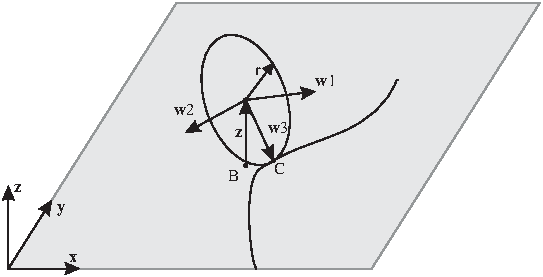
\includegraphics[height=4cm]{figures/ObjectJointRollingDiscSketch.pdf}
    \end{center}
    First, the contact point $\LU{0}{\pv}_{C}$ must be computed.
    %Using the point B which is the disc center point projeced to ground plane,
    %\be
    %  \LU{0}{\pv}_{B} = \vr{\LU{0}{\pv}_{m1,x}}{\LU{0}{\pv}_{m1,y}}{0}
    %\ee
    %This provides the vector $\dv$,
    %\be
    %  \LU{0}{\dv} = \vr{0}{0}{\LU{0}{\pv}_{m1,z}}
    %\ee
    With the helper vector,
    \be
      \LU{0}{\xv} = \LU{0}{\wv}_1 \times \LU{0}{\vv_{PN}}
    \ee
    we obtain a disc coordinate system, representing the longitudinal direction,
    \be
      \LU{0}{\wv}_2 = \frac{1}{|\LU{0}{\xv}|} \LU{0}{\xv} 
    \ee
    and the vector to the contact point,
    \be
      \LU{0}{\wv}_3 = \LU{0}{\wv}_1 \times \LU{0}{\wv}_2
    \ee
    The contact point can be computed from
    \be
      \LU{0}{\pv}_{C} = \LU{0}{\pv}_{m1} + r \cdot \LU{0}{\wv}_3
    \ee
    The velocity of the contact point at the disc is computed from,
    \be
      \LU{0}{\vv}_{C} = \LU{0}{\vv}_{m1} + \LU{0}{\tomega}_{m1} \times (r\cdot \LU{0}{\wv}_3)
    \ee
    The connector forces at the contact point $C$ are computed as follows. 
    The normal contact force reads
    \be
      f_n = k_c \cdot \LU{0}{\pv}_{C,z} + d_c \cdot \LU{0}{\vv}_{C,z}
    \ee
    The tangential forces are computed from the inplane velocity $\vv_t = [\LU{0}{\vv}_{C,x},\, \LU{0}{\vv}_{C,y}]\tp$
    \be
      \fv_t = \tmu \cdot \phi(|\vv_t|,v_\mu) \cdot f_n \cdot \ev_t
    \ee
    with the regularization function:
    \be
      \phi(v, v_\mu) = 
        \left\{ 
        	\begin{array}{ccl}
        		(2-\frac{v}{v_\mu})\frac{v}{v_\mu} & \mathrm{if} & v \le v_\mu \\
        		1 & \mathrm{if} & v > v_\mu \\
        	\end{array}
        	\right.
    \ee
    and the direction of tangential slip
    \be
      \ev_t = \frac{\vv_t}{|\vv_t|}
    \ee
    The friction coefficient matrix $\tmu$ is computed from
    \be
      \tmu = \mp{\mu_x}{0}{0}{\mu_y}
    \ee
    where for isotropic behaviour of surface and wheel, it will give a diagonal matrix with the friction coefficient in the diagonal.
    In case that the dry friction angle $\alpha_t$ is not zero, the $\tmu$ changes to
    \be
      \tmu = \mp{\cos(\alpha_t)}{\sin(\alpha_t)}{-\sin(\alpha_t)}{\cos(\alpha_t)} \mp{\mu_x}{0}{0}{\mu_y} \mp{\cos(\alpha_t)}{-\sin(\alpha_t)}{\sin(\alpha_t)}{\cos(\alpha_t)}
    \ee
    Finally, the connector forces read in joint coordinates
    \be
      \LU{J1}{\fv} = \vr{f_{t,x}}{f_{t,y}}{f_n}
    \ee
    and in global coordinates, they are computed from
    \be
      \LU{0}{\fv} = f_{t,x}\wv_l + f_{t,y} \wv_2 + f_n \vv_{PN}
    \ee
    The moment caused by the contact forces are given as
    \be
      \LU{0}{\fv} = (r\cdot \LU{0}{\wv}_3) \times \LU{0}{\fv}
    \ee
    if \texttt{activeConnector = False}, 
    \be
      \LU{J1}{\fv} = \Null
    \ee
\newpage

%+++++++++++++++++++++++++++++++++++
\mysubsubsection{ObjectContactCoordinate}
A penalty-based contact condition for one coordinate; the contact gap $g$ is defined as $g=marker.value[1]- marker.value[0] - offset$; the contact force $f_c$ is zero for $gap>0$ and otherwise computed from $f_c = g*contactStiffness + \dot g*contactDamping$; during Newton iterations, the contact force is actived only, if $dataCoordinate[0] <= 0$; dataCoordinate is set equal to gap in nonlinear iterations, but not modified in Newton iterations.\vspace{12pt}
 \\{\bf Additional information for ObjectContactCoordinate}:
\bi
  \item The Object has the following types = \texttt{Connector}
  \item Requested marker type = \texttt{Coordinate}
  \item Requested node type = \texttt{GenericData}
\ei
\vspace{12pt} \noindent The item {\bf ObjectContactCoordinate} with type = 'ContactCoordinate' has the following parameters:\vspace{-1cm}\\ 
%reference manual TABLE
\begin{center}
  \footnotesize
  \begin{longtable}{| p{4.5cm} | p{2.5cm} | p{0.5cm} | p{2.5cm} | p{6cm} |}
    \hline
    \bf Name & \bf type & \bf size & \bf default value & \bf description \\ \hline
    name &     String &      &     '' &     connector's unique name\\ \hline
    markerNumbers &     ArrayIndex &      &     [ MAXINT, MAXINT ] &     markers define contact gap\\ \hline
    nodeNumber &     Index &      &     MAXINT &     node number of a NodeGenericData for 1 dataCoordinate (used for active set strategy ==> holds the gap of the last discontinuous iteration)\\ \hline
    contactStiffness &     UReal &      &     0. &     contact (penalty) stiffness [SI:N/m]; acts only upon penetration\\ \hline
    contactDamping &     UReal &      &     0. &     contact damping [SI:N/(m s)]; acts only upon penetration\\ \hline
    offset &     UReal &      &     0. &     offset [SI:m] of contact\\ \hline
    activeConnector &     bool &      &     True &     flag, which determines, if the connector is active; used to deactivate (temorarily) a connector or constraint\\ \hline
    visualization & VObjectContactCoordinate & & & parameters for visualization of item \\ \hline
	  \end{longtable}
	\end{center}
The item VObjectContactCoordinate has the following parameters:\vspace{-1cm}\\ 
%reference manual TABLE
\begin{center}
  \footnotesize
  \begin{longtable}{| p{4.5cm} | p{2.5cm} | p{0.5cm} | p{2.5cm} | p{6cm} |}
    \hline
    \bf Name & \bf type & \bf size & \bf default value & \bf description \\ \hline
    show &     Bool &      &     True &     set true, if item is shown in visualization and false if it is not shown\\ \hline
    drawSize &     float &      &     -1. &     drawing size = diameter of spring; size == -1.f means that default connector size is used\\ \hline
    color &     Float4 &      &     [-1.,-1.,-1.,-1.] &     RGBA connector color; if R==-1, use default color\\ \hline
	  \end{longtable}
	\end{center}
\newpage

%+++++++++++++++++++++++++++++++++++
\mysubsubsection{ObjectContactCircleCable2D}
A very specialized penalty-based contact condition between a 2D circle (=marker0, any Position-marker) on a body and an ANCFCable2DShape (=marker1, Marker: BodyCable2DShape), in xy-plane; a node NodeGenericData is required with the number of cordinates according to the number of contact segments; the contact gap $g$ is integrated (piecewise linear) along the cable and circle; the contact force $f_c$ is zero for $gap>0$ and otherwise computed from $f_c = g*contactStiffness + \dot g*contactDamping$; during Newton iterations, the contact force is actived only, if $dataCoordinate[0] <= 0$; dataCoordinate is set equal to gap in nonlinear iterations, but not modified in Newton iterations.\vspace{12pt}
 \\{\bf Additional information for ObjectContactCircleCable2D}:
\bi
  \item The Object has the following types = \texttt{Connector}
  \item Requested marker type = \texttt{\_None}
  \item Requested node type = \texttt{GenericData}
\ei
\vspace{12pt} \noindent The item {\bf ObjectContactCircleCable2D} with type = 'ContactCircleCable2D' has the following parameters:\vspace{-1cm}\\ 
%reference manual TABLE
\begin{center}
  \footnotesize
  \begin{longtable}{| p{4.5cm} | p{2.5cm} | p{0.5cm} | p{2.5cm} | p{6cm} |}
    \hline
    \bf Name & \bf type & \bf size & \bf default value & \bf description \\ \hline
    name &     String &      &     '' &     connector's unique name\\ \hline
    markerNumbers &     ArrayIndex &      &     [ MAXINT, MAXINT ] &     markers define contact gap\\ \hline
    nodeNumber &     Index &      &     MAXINT &     node number of a NodeGenericData for nSegments dataCoordinates (used for active set strategy ==> hold the gap of the last discontinuous iteration and the friction state)\\ \hline
    numberOfContactSegments &     Index &      &     3 &     number of linear contact segments to determine contact; each segment is a line and is associated to a data (history) variable; must be same as in according marker\\ \hline
    contactStiffness &     UReal &      &     0. &     contact (penalty) stiffness [SI:N/m/(contact segment)]; the stiffness is per contact segment; specific contact forces (per length) $f_N$ act in contact normal direction only upon penetration\\ \hline
    contactDamping &     UReal &      &     0. &     contact damping [SI:N/(m s)/(contact segment)]; the damping is per contact segment; acts in contact normal direction only upon penetration\\ \hline
    circleRadius &     UReal &      &     0. &     radius [SI:m] of contact circle\\ \hline
    offset &     UReal &      &     0. &     offset [SI:m] of contact, e.g. to include thickness of cable element\\ \hline
    activeConnector &     bool &      &     True &     flag, which determines, if the connector is active; used to deactivate (temorarily) a connector or constraint\\ \hline
    visualization & VObjectContactCircleCable2D & & & parameters for visualization of item \\ \hline
	  \end{longtable}
	\end{center}
The item VObjectContactCircleCable2D has the following parameters:\vspace{-1cm}\\ 
%reference manual TABLE
\begin{center}
  \footnotesize
  \begin{longtable}{| p{4.5cm} | p{2.5cm} | p{0.5cm} | p{2.5cm} | p{6cm} |}
    \hline
    \bf Name & \bf type & \bf size & \bf default value & \bf description \\ \hline
    show &     Bool &      &     True &     set true, if item is shown in visualization and false if it is not shown\\ \hline
    drawSize &     float &      &     -1. &     drawing size = diameter of spring; size == -1.f means that default connector size is used\\ \hline
    color &     Float4 &      &     [-1.,-1.,-1.,-1.] &     RGBA connector color; if R==-1, use default color\\ \hline
	  \end{longtable}
	\end{center}
\newpage

%+++++++++++++++++++++++++++++++++++
\mysubsubsection{ObjectContactFrictionCircleCable2D}
A very specialized penalty-based contact/friction condition between a 2D circle in the local x/y plane (=marker0, a Rigid-Body Marker) on a body and an ANCFCable2DShape (=marker1, Marker: BodyCable2DShape), in xy-plane; a node NodeGenericData is required with 3$\times$(number of contact segments) -- containing per segment: [contact gap, stick/slip (stick=1), last friction position]; the contact gap $g$ is integrated (piecewise linear) along the cable and circle; the contact force $f_c$ is zero for $gap>0$ and otherwise computed from $f_c = g*contactStiffness + \dot g*contactDamping$; during Newton iterations, the contact force is actived only, if $dataCoordinate[0] <= 0$; dataCoordinate is set equal to gap in nonlinear iterations, but not modified in Newton iterations.\vspace{12pt}
 \\{\bf Additional information for ObjectContactFrictionCircleCable2D}:
\bi
  \item The Object has the following types = \texttt{Connector}
  \item Requested marker type = \texttt{\_None}
  \item Requested node type = \texttt{GenericData}
\ei
\vspace{12pt} \noindent The item {\bf ObjectContactFrictionCircleCable2D} with type = 'ContactFrictionCircleCable2D' has the following parameters:\vspace{-1cm}\\ 
%reference manual TABLE
\begin{center}
  \footnotesize
  \begin{longtable}{| p{4.5cm} | p{2.5cm} | p{0.5cm} | p{2.5cm} | p{6cm} |}
    \hline
    \bf Name & \bf type & \bf size & \bf default value & \bf description \\ \hline
    name &     String &      &     '' &     connector's unique name\\ \hline
    markerNumbers &     ArrayIndex &      &     [ MAXINT, MAXINT ] &     markers define contact gap\\ \hline
    nodeNumber &     Index &      &     MAXINT &     node number of a NodeGenericData with 3 $\times$ nSegments dataCoordinates (used for active set strategy ==> hold the gap of the last discontinuous iteration and the friction state)\\ \hline
    numberOfContactSegments &     Index &      &     3 &     number of linear contact segments to determine contact; each segment is a line and is associated to a data (history) variable; must be same as in according marker\\ \hline
    contactStiffness &     UReal &      &     0. &     contact (penalty) stiffness [SI:N/m/(contact segment)]; the stiffness is per contact segment; specific contact forces (per length) $f_N$ act in contact normal direction only upon penetration\\ \hline
    contactDamping &     UReal &      &     0. &     contact damping [SI:N/(m s)/(contact segment)]; the damping is per contact segment; acts in contact normal direction only upon penetration\\ \hline
    frictionVelocityPenalty &     UReal &      &     0. &     velocity dependent penalty coefficient for friction [SI:N/(m s)/(contact segment)]; the coefficient causes tangential (contact) forces against relative tangential velocities in the contact area\\ \hline
    frictionStiffness &     UReal &      &     0. &     CURRENTLY NOT IMPLEMENTED: displacement dependent penalty/stiffness coefficient for friction [SI:N/m/(contact segment)]; the coefficient causes tangential (contact) forces against relative tangential displacements in the contact area\\ \hline
    frictionCoefficient &     UReal &      &     0. &     friction coefficient $\mu$ [SI: 1]; tangential specific friction forces (per length) $f_T$ must fulfill the condition $f_T \le \mu f_N$\\ \hline
    circleRadius &     UReal &      &     0. &     radius [SI:m] of contact circle\\ \hline
    offset &     UReal &      &     0. &     offset [SI:m] of contact, e.g. to include thickness of cable element\\ \hline
    activeConnector &     bool &      &     True &     flag, which determines, if the connector is active; used to deactivate (temorarily) a connector or constraint\\ \hline
    visualization & VObjectContactFrictionCircleCable2D & & & parameters for visualization of item \\ \hline
	  \end{longtable}
	\end{center}
The item VObjectContactFrictionCircleCable2D has the following parameters:\vspace{-1cm}\\ 
%reference manual TABLE
\begin{center}
  \footnotesize
  \begin{longtable}{| p{4.5cm} | p{2.5cm} | p{0.5cm} | p{2.5cm} | p{6cm} |}
    \hline
    \bf Name & \bf type & \bf size & \bf default value & \bf description \\ \hline
    show &     Bool &      &     True &     set true, if item is shown in visualization and false if it is not shown\\ \hline
    drawSize &     float &      &     -1. &     drawing size = diameter of spring; size == -1.f means that default connector size is used\\ \hline
    color &     Float4 &      &     [-1.,-1.,-1.,-1.] &     RGBA connector color; if R==-1, use default color\\ \hline
	  \end{longtable}
	\end{center}
\newpage

%+++++++++++++++++++++++++++++++++++
\mysubsubsection{ObjectJointGeneric}
A generic joint in 3D; constrains components of the absolute position and rotations of two points given by PointMarkers or RigidMarkers; an additional local rotation can be used to define three rotation axes and/or sliding axes\vspace{12pt}
 \\{\bf Additional information for ObjectJointGeneric}:
\bi
  \item The Object has the following types = \texttt{Connector}, \texttt{Constraint}
  \item Requested marker type = \texttt{Position} + \texttt{Orientation}
  \item {\bf Short name} for Python = {\bf GenericJoint}  \item {\bf Short name} for Python (visualization object) = {\bf VGenericJoint}\ei
\vspace{12pt} \noindent The item {\bf ObjectJointGeneric} with type = 'JointGeneric' has the following parameters:\vspace{-1cm}\\ 
%reference manual TABLE
\begin{center}
  \footnotesize
  \begin{longtable}{| p{4.5cm} | p{2.5cm} | p{0.5cm} | p{2.5cm} | p{6cm} |}
    \hline
    \bf Name & \bf type & \bf size & \bf default value & \bf description \\ \hline
    name &     String &      &     '' &     constraints's unique name\\ \hline
    markerNumbers &     ArrayIndex &     2 &     [ MAXINT, MAXINT ] &     list of markers used in connector\\ \hline
    constrainedAxes &     ArrayIndex &     6 &     [1,1,1,1,1,1] &     flag, which determines which translation (0,1,2) and rotation (3,4,5) axes are constrained; for $j_i$, two values are possible: 0=free axis, 1=constrained axis\\ \hline
    rotationMarker0 &     Matrix3D &      &     [[1,0,0], [0,1,0], [0,0,1]] &     local rotation matrix for marker $m0$; translation and rotation axes for marker $m0$ are defined in the local body coordinate system and additionally transformed by rotationMarker0\\ \hline
    rotationMarker1 &     Matrix3D &      &     [[1,0,0], [0,1,0], [0,0,1]] &     local rotation matrix for marker $m1$; translation and rotation axes for marker $m1$ are defined in the local body coordinate system and additionally transformed by rotationMarker1\\ \hline
    activeConnector &     bool &      &     True &     flag, which determines, if the connector is active; used to deactivate (temorarily) a connector or constraint\\ \hline
    offsetUserFunctionParameters &     Vector6D &      &     [0.,0.,0.,0.,0.,0.] &     vector of 6 parameters for joint's offsetUserFunction\\ \hline
    offsetUserFunction &     PyFunctionVector6DScalarVector6D &     \tabnewline  &     \tabnewline 0 &     A python function which defines the time-dependent (fixed) offset of translation (indices 0,1,2) and rotation (indices 3,4,5) joint coordinates with parameters (t, offsetUserFunctionParameters); the offset represents the current value of the object; it is highly RECOMMENDED to use sufficiently smooth functions, having consistent initial offsets with initial configuration of bodies, zero or compatible initial offset-velocity, and no accelerations; Example for python function: def f(t, offsetUserFunctionParameters): return [offsetUserFunctionParameters[0]*(1 - np.cos(t*10*2*np.pi)), 0,0,0,0,0]\\ \hline
    offsetUserFunction\_t &     PyFunctionVector6DScalarVector6D &     \tabnewline  &     \tabnewline 0 &     (NOT IMPLEMENTED YET)time derivative of offsetUserFunction using the same parameters; needed for 'velocityLevel=True', or for index2 time integration and for computation of initial accelerations in SecondOrderImplicit integrators\\ \hline
    visualization & VObjectJointGeneric & & & parameters for visualization of item \\ \hline
	  \end{longtable}
	\end{center}
The item VObjectJointGeneric has the following parameters:\vspace{-1cm}\\ 
%reference manual TABLE
\begin{center}
  \footnotesize
  \begin{longtable}{| p{4.5cm} | p{2.5cm} | p{0.5cm} | p{2.5cm} | p{6cm} |}
    \hline
    \bf Name & \bf type & \bf size & \bf default value & \bf description \\ \hline
    show &     bool &      &     True &     set true, if item is shown in visualization and false if it is not shown\\ \hline
    axesRadius &     float &      &     0.1 &     radius of joint axes to draw\\ \hline
    axesLength &     float &      &     0.4 &     length of joint axes to draw\\ \hline
    color &     Float4 &      &     [-1.,-1.,-1.,-1.] &     RGBA connector color; if R==-1, use default color\\ \hline
	  \end{longtable}
	\end{center}
{\bf Detailed information on ObjectJointGeneric}:
\startTable{input parameter}{symbol}{description see tables above}
\rowTable{markerNumbers}{$[m0,m1]\tp$}{}
\rowTable{constrainedAxes}{$\jv=[j_0,\,\ldots,\,j_5]$}{}
\rowTable{rotationMarker0}{$\LU{m0,J0}{\Rot}$}{}
\rowTable{rotationMarker1}{$\LU{m1,J1}{\Rot}$}{}
\rowTable{offsetUserFunctionParameters}{$\pv_{par}$}{}
\rowTable{offsetUserFunction}{$UF(t, \pv_{par})$}{}
\rowTable{offsetUserFunction\_t}{$UF_t(t, \pv_{par})$}{}
\finishTable
{\bf The following output parameters are available as OutputVariableType in sensors and other functions}: 
\startTable{output parameter}{symbol}{description}
\rowTable{Position}{$\LU{0}{\pv}_{m0}$}{current global position of position marker $m0$}
\rowTable{Velocity}{$\LU{0}{\vv}_{m0}$}{current global velocity of position marker $m0$}
\rowTable{DisplacementLocal}{$\LU{J0}{\Delta\pv}$}{relative displacement in local joint0 coordinates; uses local J0 coordinates even for spherical joint configuration}
\rowTable{VelocityLocal}{$\LU{J0}{\Delta\vv}$}{relative translational velocity in local joint0 coordinates}
\rowTable{Rotation}{$\LU{J0}{\ttheta}= [\theta_0,\theta_1,\theta_2]\tp$}{relative rotation parameters (Tait Bryan Rxyz); if all axes are fixed, this output represents the rotational drift; for a revolute joint, it contains the rotation of this axis}
\rowTable{AngularVelocityLocal}{$\LU{J0}{\Delta\tomega}$}{relative angular velocity in local joint0 coordinates; if all axes are fixed, this output represents the angular velocity constraint error; for a revolute joint, it contains the angular velocity of this axis}
\rowTable{ForceLocal}{$\LU{J0}{\fv}$}{joint force in local $J0$ coordinates}
\rowTable{TorqueLocal}{$\LU{J0}{\mv}$}{joint torque in local $J0$ coordinates; depending on joint configuration, the result may not be the according torque vector}
\finishTable
{\bf Description of Item}:
 \noindent
    \vspace{6pt}\\
    {\bf Definition of quantities}:
    \startTable{intermediate variables}{symbol}{description}
    \rowTable{marker m0 position}{$\LU{0}{\pv}_{m0}$}{current global position which is provided by marker m0}
    \rowTable{marker m0 orientation}{$\LU{0,m0}{\Rot}$}{current rotation matrix provided by marker m0}
    \rowTable{joint J0 orientation}{$\LU{0,J0}{\Rot} = \LU{0,m0}{\Rot} \LU{m0,J0}{\Rot}$}{joint $J0$ rotation matrix}
    \rowTable{joint J0 orientation vectors}{$\LU{0,J0}{\Rot} = [\vv_{x0},\,\vv_{y0},\,\vv_{z0}]\tp$}{orientation vectors used for definition of constraint equations}
    \rowTable{marker m1 position}{$\LU{0}{\pv}_{m1}$}{accordingly}
    \rowTable{marker m1 orientation}{$\LU{0,m1}{\Rot}$}{current rotation matrix provided by marker m1}
    \rowTable{joint J1 orientation}{$\LU{0,J1}{\Rot} = \LU{0,m1}{\Rot} \LU{m1,J1}{\Rot}$}{joint $J1$ rotation matrix}
    \rowTable{joint J1 orientation vectors}{$\LU{0,J1}{\Rot} = [\vv_{x1},\,\vv_{y1},\,\vv_{z1}]\tp$}{orientation vectors used for definition of constraint equations}

%
    \rowTable{marker m0 velocity}{$\LU{0}{\vv}_{m0}$}{current global velocity which is provided by marker m0}
    \rowTable{marker m1 velocity}{$\LU{0}{\vv}_{m1}$}{accordingly}
    \rowTable{marker m0 velocity}{$\LU{b}{\tomega}_{m0}$}{current local angular velocity vector provided by marker m0}
    \rowTable{marker m1 velocity}{$\LU{b}{\tomega}_{m1}$}{current local angular velocity vector provided by marker m1}
    \rowTable{Displacement}{$\LU{0}{\Delta\pv}=\LU{0}{\pv}_{m1} - \LU{0}{\pv}_{m0}$} {used, if all translational axes are constrained}
    \rowTable{Velocity}{$\LU{0}{\Delta\vv} = \LU{0}{\vv}_{m1} - \LU{0}{\vv}_{m0}$}{used, if all translational axes are constrained (velocity level)}
%
    \rowTable{DisplacementLocal}{$\LU{J0}{\Delta\pv}$}{$\left(\LU{0,m0}{\Rot}\LU{m0,J0}{\Rot}\right)\tp \LU{0}{\Delta\pv}$}
    \rowTable{VelocityLocal}{$\LU{J0}{\Delta\vv}$}{$\left(\LU{0,m0}{\Rot}\LU{m0,J0}{\Rot}\right)\tp \LU{0}{\Delta\vv}$ $\ldots$ note that this is the global relative velocity projected into the local $J0$ coordinate system}
    \rowTable{AngularVelocityLocal}{$\LU{J0}{\Delta\omega}$}{$\left(\LU{0,m0}{\Rot}\LU{m0,J0}{\Rot}\right)\tp \left( \LU{0,m1}{\Rot} \LU{m1}{\omega} - \LU{0,m0}{\Rot} \LU{m0}{\omega} \right)$}
    \rowTable{algebraic variables}{$\zv=[\lambda_0,\,\ldots,\,\lambda_5]\tp$}{vector of algebraic variables (Lagrange multipliers) according to the algebraic equations}
    \finishTable
    \vspace{6pt}
    \noindent {\bf Connector equations for translational part (\texttt{activeConnector = True})}:\\
    %++++++++++++++++++++++++++++++++++++++++++++++++++++++++++
    If $[j_0,\,\ldots,\,j_2] = [1,1,1]\tp$, meaning that all translational coordinates are fixed,
    the translational index 3 constraints read ($UF_{0,1,2}(t, \pv_{par})$ is the translational part of the user function $UF$),
    \be
      \LU{0}{\pv}_{m1} - \LU{0}{\pv}_{m0} - UF_{0,1,2}(t, \pv_{par}) = \Null
    \ee
    and the translational index 2 constraints read
    \be
      \LU{0}{\vv}_{m1} - \LU{0}{\vv}_{m0} - UF_{t;0,1,2}(t, \pv_{par})= \Null    
    \ee
    %++++++++++++++++++++++++++++++++++++++++++++++++++++++++++
    If $[j_0,\,\ldots,\,j_2] \neq [1,1,1]\tp$, meaning that at least one translational coordinate is free,
    the translational index 3 constraints read for every component $k \in [0,1,2]$ of the vector $\LU{J0}{\Delta\pv}$
    \bea
      \LU{J0}{\Delta p_k} - UF_{k}(t, \pv_{par}) &=& 0 \quad \mathrm{if} \quad j_k = 1 \quad \mathrm{and}\\
      \lambda_k &=& 0 \quad \mathrm{if} \quad j_k = 0 \\
    \eea
    and the translational index 2 constraints read for every component $k \in [0,1,2]$ of the vector $\LU{J0}{\Delta\vv}$
    \bea
      \LU{J0}{\Delta v_k} - UF_{t;k}(t, \pv_{par})  &=& 0 \quad \mathrm{if} \quad j_k = 1 \quad \mathrm{and}\\
      \lambda_k &=& 0 \quad \mathrm{if} \quad j_k = 0 \\
    \eea
%
    %++++++++++++++++++++++++++++++++++++++++++++++++++++++++++
    \noindent {\bf Connector equations for rotational part (\texttt{activeConnector = True})}:\\
    The following equations are exemplarily for certain constrained rotation axes configurations, which shall represent all other possibilities.
    Equations are only given for the index 3 case; the index 2 case can be derived from these equations easily (see C++ code...).
    In case of user functions, the additional rotation matrix $\LU{J0,J0U}{\Rot}(UF_{3,4,5}(t, \pv_{par}))$, in which the three components of 
    $UF_{3,4,5}$ are interpreted as Tait-Bryan angles that are added to the joint frame.
    
    If {\bf 3 rotation axes are constrained},  $[j_3,\,\ldots,\,j_5] = [1,1,1]\tp$, the index 3 constraint equations read
    \bea
       \vv_{z0}\tp \vv_{y1} &=& 0 \\
       \vv_{z0}\tp \vv_{x1} &=& 0 \\
       \vv_{x0}\tp \vv_{y1} &=& 0
    \eea
    If {\bf 2 rotation axes are constrained}, e.g., $[j_3,\,\ldots,\,j_5] = [0,1,1]\tp$, the index 3 constraint equations read
    \bea
       \lambda_3 &=& 0 \\
       \vv_{x0}\tp \vv_{y1} &=& 0 \\
       \vv_{x0}\tp \vv_{z1} &=& 0
    \eea
    If {\bf 1 rotation axis is constrained}, e.g.,  $[j_3,\,\ldots,\,j_5] = [1,0,0]\tp$, the index 3 constraint equations read
    \bea
       \vv_{y0}\tp \vv_{z1} &=& 0 \\
       \lambda_4 &=& 0 \\
       \lambda_5 &=& 0
    \eea
%    
    if \texttt{activeConnector = False}, 
    \be
      \zv = \Null
    \ee
\newpage

%+++++++++++++++++++++++++++++++++++
\mysubsubsection{ObjectJointSpherical}
A spherical joint, which constrains the relative translation between two position based markers.\vspace{12pt}
 \\{\bf Additional information for ObjectJointSpherical}:
\bi
  \item The Object has the following types = \texttt{Connector}, \texttt{Constraint}
  \item Requested marker type = \texttt{Position}
  \item {\bf Short name} for Python = {\bf SphericalJoint}  \item {\bf Short name} for Python (visualization object) = {\bf VSphericalJoint}\ei
\vspace{12pt} \noindent The item {\bf ObjectJointSpherical} with type = 'JointSpherical' has the following parameters:\vspace{-1cm}\\ 
%reference manual TABLE
\begin{center}
  \footnotesize
  \begin{longtable}{| p{4.5cm} | p{2.5cm} | p{0.5cm} | p{2.5cm} | p{6cm} |}
    \hline
    \bf Name & \bf type & \bf size & \bf default value & \bf description \\ \hline
    name &     String &      &     '' &     constraints's unique name\\ \hline
    markerNumbers &     ArrayIndex &     2 &     [ MAXINT, MAXINT ] &     list of markers used in connector\\ \hline
    constrainedAxes &     ArrayIndex &     3 &     [1,1,1] &     flag, which determines which translation (0,1,2) and rotation (3,4,5) axes are constrained; for $j_i$, two values are possible: 0=free axis, 1=constrained axis\\ \hline
    activeConnector &     bool &      &     True &     flag, which determines, if the connector is active; used to deactivate (temorarily) a connector or constraint\\ \hline
    visualization & VObjectJointSpherical & & & parameters for visualization of item \\ \hline
	  \end{longtable}
	\end{center}
The item VObjectJointSpherical has the following parameters:\vspace{-1cm}\\ 
%reference manual TABLE
\begin{center}
  \footnotesize
  \begin{longtable}{| p{4.5cm} | p{2.5cm} | p{0.5cm} | p{2.5cm} | p{6cm} |}
    \hline
    \bf Name & \bf type & \bf size & \bf default value & \bf description \\ \hline
    show &     bool &      &     True &     set true, if item is shown in visualization and false if it is not shown\\ \hline
    jointRadius &     float &      &     0.1 &     radius of joint to draw\\ \hline
    color &     Float4 &      &     [-1.,-1.,-1.,-1.] &     RGBA connector color; if R==-1, use default color\\ \hline
	  \end{longtable}
	\end{center}
{\bf Detailed information on ObjectJointSpherical}:
\startTable{input parameter}{symbol}{description see tables above}
\rowTable{markerNumbers}{$[m0,m1]\tp$}{}
\rowTable{constrainedAxes}{$\jv=[j_0,\,\ldots,\,j_2]$}{}
\finishTable
{\bf The following output parameters are available as OutputVariableType in sensors and other functions}: 
\startTable{output parameter}{symbol}{description}
\rowTable{Position}{$\LU{0}{\pv}_{m0}$}{current global position of position marker $m0$}
\rowTable{Velocity}{$\LU{0}{\vv}_{m0}$}{current global velocity of position marker $m0$}
\rowTable{Displacement}{$\LU{0}{\Delta\pv}=\LU{0}{\pv}_{m1} - \LU{0}{\pv}_{m0}$}{constraint drift or relative motion, if not all axes fixed}
\rowTable{Force}{$\LU{0}{\fv}$}{joint force in global coordinates}
\finishTable
{\bf Description of Item}:
 \noindent
    \vspace{6pt}\\
    {\bf Definition of quantities}:
    \startTable{intermediate variables}{symbol}{description}
    \rowTable{marker m0 position}{$\LU{0}{\pv}_{m0}$}{current global position which is provided by marker $m0$}
    \rowTable{marker m1 position}{$\LU{0}{\pv}_{m1}$}{current global position which is provided by marker $m1$}
    \rowTable{marker m0 velocity}{$\LU{0}{\vv}_{m0}$}{current global velocity which is provided by marker $m0$}
    \rowTable{marker m1 velocity}{$\LU{0}{\vv}_{m1}$}{current global velocity which is provided by marker $m1$}
%
    \rowTable{relative velocity}{$\LU{0}{\Delta\vv} = \LU{0}{\vv}_{m1} - \LU{0}{\vv}_{m0}$}{constraint velocity error, or relative velocity if not all axes fixed}
%
    \rowTable{algebraic variables}{$\zv=[\lambda_0,\,\ldots,\,\lambda_2]\tp$}{vector of algebraic variables (Lagrange multipliers) according to the algebraic equations}
    \finishTable
%
    \vspace{6pt}
    \noindent {\bf Connector equations (\texttt{activeConnector = True})}:\\
    %++++++++++++++++++++++++++++++++++++++++++++++++++++++++++
    If $[j_0,\,\ldots,\,j_2] = [1,1,1]\tp$, meaning that all translational coordinates are fixed,
    the translational index 3 constraints read
    \be
      \LU{0}{\pv}_{m1} - \LU{0}{\pv}_{m0} = \Null
    \ee
    and the translational index 2 constraints read
    \be
      \LU{0}{\vv}_{m1} - \LU{0}{\vv}_{m0} = \Null    
    \ee
    %++++++++++++++++++++++++++++++++++++++++++++++++++++++++++
    If $[j_0,\,\ldots,\,j_2] \neq [1,1,1]\tp$, meaning that at least one translational coordinate is free,
    the translational index 3 constraints read for every component $k \in [0,1,2]$ of the vector $\LU{0}{\Delta\pv}$
    \bea
      \LU{0}{\Delta p_k} &=& 0 \quad \mathrm{if} \quad j_k = 1 \quad \mathrm{and}\\
      \lambda_k &=& 0 \quad \mathrm{if} \quad j_k = 0 \\
    \eea
    and the translational index 2 constraints read for every component $k \in [0,1,2]$ of the vector $\LU{0}{\Delta\vv}$
    \bea
      \LU{0}{\Delta v_k} &=& 0 \quad \mathrm{if} \quad j_k = 1 \quad \mathrm{and}\\
      \lambda_k &=& 0 \quad \mathrm{if} \quad j_k = 0 \\
    \eea
%
    if \texttt{activeConnector = False}, 
    \be
      \zv = \Null
    \ee
\newpage

%+++++++++++++++++++++++++++++++++++
\mysubsubsection{ObjectJointRollingDisc}
A joint representing a rolling rigid disc (marker 1) on a flat surface (marker 0, ground body) in global $x$-$y$ plane. The contraint is based on an idealized rolling formulation with no slip. The contraints works for discs as long as the disc axis and the plane normal vector are not parallel. It must be assured that the disc has contact to ground in the initial configuration (adjust z-position of body accordingly).\vspace{12pt}
 \\{\bf Additional information for ObjectJointRollingDisc}:
\bi
  \item The Object has the following types = \texttt{Connector}, \texttt{Constraint}
  \item Requested marker type = \texttt{Position} + \texttt{Orientation}
  \item {\bf Short name} for Python = {\bf RollingDiscJoint}  \item {\bf Short name} for Python (visualization object) = {\bf VRollingDiscJoint}\ei
\vspace{12pt} \noindent The item {\bf ObjectJointRollingDisc} with type = 'JointRollingDisc' has the following parameters:\vspace{-1cm}\\ 
%reference manual TABLE
\begin{center}
  \footnotesize
  \begin{longtable}{| p{4.5cm} | p{2.5cm} | p{0.5cm} | p{2.5cm} | p{6cm} |}
    \hline
    \bf Name & \bf type & \bf size & \bf default value & \bf description \\ \hline
    name &     String &      &     '' &     constraints's unique name\\ \hline
    markerNumbers &     ArrayIndex &     2 &     [ MAXINT, MAXINT ] &     list of markers used in connector\\ \hline
    constrainedAxes &     ArrayIndex &     3 &     [1,1,1] &     flag, which determines which constraints are active, in which $j_0,j_1$ represent the tangential motion and $j_2$ represents the normal (contact) direction\\ \hline
    activeConnector &     bool &      &     True &     flag, which determines, if the connector is active; used to deactivate (temorarily) a connector or constraint\\ \hline
    discRadius &     Real &      &     0 &     defines the disc radius\\ \hline
    visualization & VObjectJointRollingDisc & & & parameters for visualization of item \\ \hline
	  \end{longtable}
	\end{center}
The item VObjectJointRollingDisc has the following parameters:\vspace{-1cm}\\ 
%reference manual TABLE
\begin{center}
  \footnotesize
  \begin{longtable}{| p{4.5cm} | p{2.5cm} | p{0.5cm} | p{2.5cm} | p{6cm} |}
    \hline
    \bf Name & \bf type & \bf size & \bf default value & \bf description \\ \hline
    show &     bool &      &     True &     set true, if item is shown in visualization and false if it is not shown\\ \hline
    discWidth &     float &      &     0.1 &     width of disc for drawing\\ \hline
    color &     Float4 &      &     [-1.,-1.,-1.,-1.] &     RGBA connector color; if R==-1, use default color\\ \hline
	  \end{longtable}
	\end{center}
{\bf Detailed information on ObjectJointRollingDisc}:
\startTable{input parameter}{symbol}{description see tables above}
\rowTable{markerNumbers}{$[m0,m1]\tp$}{}
\rowTable{constrainedAxes}{$\jv=[j_0,\,\ldots,\,j_2]$}{}
\finishTable
{\bf The following output parameters are available as OutputVariableType in sensors and other functions}: 
\startTable{output parameter}{symbol}{description}
\rowTable{Position}{$\LU{0}{\pv}_{G}$}{current global position of contact point between rolling disc and ground}
\rowTable{VelocityLocal}{$\LU{D}{\vv}_{G}$}{current velocity of the trail (contact) point in disc coordinates; this is the velocity with which the contact moves over the ground plane}
\rowTable{ForceLocal}{$\LU{D}{\fv} = [-\zv^T \wv_l, \, -\zv^T \wv_2, \, -\zv_z]\tp$}{contact forces acting on disc, in special disc coordinates, $f_x$ being the lateral force, $f_y$ being the longitudinal force and $f_z$ being the normal force}
\finishTable
{\bf Description of Item}:
 \noindent
    \vspace{6pt}\\
    {\bf Definition of quantities}:
    \startTable{intermediate variables}{symbol}{description}
    \rowTable{marker m0 position}{$\LU{0}{\pv}_{m0}$}{current global position which is provided by marker m0, any ground reference position; currently unused}
    \rowTable{marker m0 orientation}{$\LU{0,m0}{\Rot}$}{current rotation matrix provided by marker m0; currently unused}
    \rowTable{marker m1 position}{$\LU{0}{\pv}_{m1}$}{center of disc}
    \rowTable{marker m1 orientation}{$\LU{0,m1}{\Rot}$}{current rotation matrix provided by marker m1}
%
    %\rowTable{marker m0 velocity}{$\LU{0}{\vv}_{m0}$}{current global velocity which is provided by marker m0}
    \rowTable{marker m1 velocity}{$\LU{0}{\vv}_{m1}$}{accordingly}
    %\rowTable{marker m0 angular velocity}{$\LU{0}{\tomega}_{m0}$}{current angular velocity vector provided by marker m0}
    \rowTable{marker m1 angular velocity}{$\LU{0}{\tomega}_{m1}$}{current angular velocity vector provided by marker m1}
%
    \rowTable{ground normal vector}{$\LU{0}{\vv_{PN}}$}{normalized normal vector to the ground plane, currently [0,0,1]}
    \rowTable{ground position B}{$\LU{0}{\pv}_{B}$}{disc center point projected on ground (normal projection)}
    \rowTable{ground position C}{$\LU{0}{\pv}_{C}$}{contact point of disc with ground}
    \rowTable{ground velocity C}{$\LU{0}{\vv}_{C}$}{velocity of disc at ground contact point (must be zero at end of iteration)}
    %\rowTable{ground vector}{$\LU{0}{\dv}$}{vector from ground to the disc center point , currently [0,0,\LU{0}{\pv}_{m1,z}]}
    \rowTable{wheel axis vector}{$\LU{0}{\wv}_1 =\LU{0,m1}{\Rot} \cdot [1,0,0]\tp $}{normalized disc axis vector, currently $[1,0,0]\tp$ in local coordinates}
    \rowTable{longitudinal vector}{$\LU{0}{\wv}_2$}{vector in longitudinal (motion) direction}
    \rowTable{lateral vector}{$\LU{0}{\wv}_l = \LU{0}{\vv_{PN}} \times \LU{0}{\wv}_2 = [-\wv_{2,y}, \wv_{2,x}, 0]$}{vector in lateral direction, lies in ground plane}
    \rowTable{contact point vector}{$\LU{0}{\wv}_3$}{normalized vector from disc center point in direction of contact point C}
%
    \rowTable{algebraic variables}{$\zv=[\lambda_0,\,\lambda_1,\,\lambda_2]\tp$}{vector of algebraic variables (Lagrange multipliers) according to the algebraic equations}
    \finishTable
    \vspace{6pt}
    \noindent {\bf Geometric relations}:\\
    %++++++++++++++++++++++++++++++++++++++++++++++++++++++++++
    \noindent The main geometrical setup is shown in the following figure:
    \begin{center}
        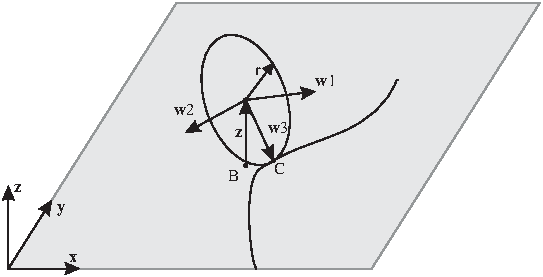
\includegraphics[height=4cm]{figures/ObjectJointRollingDiscSketch.pdf}
    \end{center}
    First, the contact point $\LU{0}{\pv}_{C}$ must be computed.
    %Using the point B which is the disc center point projeced to ground plane,
    %\be
    %  \LU{0}{\pv}_{B} = \vr{\LU{0}{\pv}_{m1,x}}{\LU{0}{\pv}_{m1,y}}{0}
    %\ee
    %This provides the vector $\dv$,
    %\be
    %  \LU{0}{\dv} = \vr{0}{0}{\LU{0}{\pv}_{m1,z}}
    %\ee
    With the helper vector,
    \be
      \LU{0}{\xv} = \LU{0}{\wv}_1 \times \LU{0}{\vv_{PN}}
    \ee
    we obtain a disc coordinate system, representing the longitudinal direction,
    \be
      \LU{0}{\wv}_2 = \frac{1}{|\LU{0}{\xv}|} \LU{0}{\xv} 
    \ee
    and the vector to the contact point,
    \be
      \LU{0}{\wv}_3 = \LU{0}{\wv}_1 \times \LU{0}{\wv}_2
    \ee
    The contact point can be computed from
    \be
      \LU{0}{\pv}_{C} = \LU{0}{\pv}_{m1} + r \cdot \LU{0}{\wv}_3
    \ee
    The velocity of the contact point at the disc is computed from,
    \be
      \LU{0}{\vv}_{C} = \LU{0}{\vv}_{m1} + \LU{0}{\tomega}_{m1} \times (r\cdot \LU{0}{\wv}_3)
    \ee
    \vspace{6pt}
    \noindent {\bf Connector constraint equations (\texttt{activeConnector = True})}:\\
    %The holonomic, index 3 constraint for the normal direction reads
    %\be
    %  \LU{0}{\pv}_{C,z} = 0
    %\ee
    The non-holonomic, index 2 constraints for the tangential motion follow from (an index 3 formulation would be possible, but is not implemented yet because of mixing different jacobians)
    \be
      \vp{\LU{0}{\vv}_{C,x}}{\LU{0}{\vv}_{C,y}}= \Null
    \ee
    In the index 2 (velocity level) case, the constraint for the normal direction reads
    \be
      \LU{0}{\vv}_{C,z} = 0
    \ee
    if \texttt{activeConnector = False}, 
    \be
      \zv = \Null
    \ee
\newpage

%+++++++++++++++++++++++++++++++++++
\mysubsubsection{ObjectJointRevolute2D}
A revolute joint in 2D; constrains the absolute 2D position of two points given by PointMarkers or RigidMarkers\vspace{12pt}
 \\{\bf Additional information for ObjectJointRevolute2D}:
\bi
  \item The Object has the following types = \texttt{Connector}, \texttt{Constraint}
  \item Requested marker type = \texttt{Position}
  \item {\bf Short name} for Python = {\bf RevoluteJoint2D}  \item {\bf Short name} for Python (visualization object) = {\bf VRevoluteJoint2D}\ei
\vspace{12pt} \noindent The item {\bf ObjectJointRevolute2D} with type = 'JointRevolute2D' has the following parameters:\vspace{-1cm}\\ 
%reference manual TABLE
\begin{center}
  \footnotesize
  \begin{longtable}{| p{4.5cm} | p{2.5cm} | p{0.5cm} | p{2.5cm} | p{6cm} |}
    \hline
    \bf Name & \bf type & \bf size & \bf default value & \bf description \\ \hline
    name &     String &      &     '' &     constraints's unique name\\ \hline
    markerNumbers &     ArrayIndex &      &     [ MAXINT, MAXINT ] &     list of markers used in connector\\ \hline
    activeConnector &     bool &      &     True &     flag, which determines, if the connector is active; used to deactivate (temorarily) a connector or constraint\\ \hline
    visualization & VObjectJointRevolute2D & & & parameters for visualization of item \\ \hline
	  \end{longtable}
	\end{center}
The item VObjectJointRevolute2D has the following parameters:\vspace{-1cm}\\ 
%reference manual TABLE
\begin{center}
  \footnotesize
  \begin{longtable}{| p{4.5cm} | p{2.5cm} | p{0.5cm} | p{2.5cm} | p{6cm} |}
    \hline
    \bf Name & \bf type & \bf size & \bf default value & \bf description \\ \hline
    show &     bool &      &     True &     set true, if item is shown in visualization and false if it is not shown\\ \hline
    drawSize &     float &      &     -1. &     drawing size = radius of revolute joint; size == -1.f means that default connector size is used\\ \hline
    color &     Float4 &      &     [-1.,-1.,-1.,-1.] &     RGBA connector color; if R==-1, use default color\\ \hline
	  \end{longtable}
	\end{center}
\newpage

%+++++++++++++++++++++++++++++++++++
\mysubsubsection{ObjectJointPrismatic2D}
A prismatic joint in 2D; allows the relative motion of two bodies, using two RigidMarkers; the vector $\tv_0$ = axisMarker0 is given in local coordinates of the first marker's (body) frame and defines the prismatic axis; the vector $\mathbf{n}_1$ = normalMarker1 is given in the second marker's (body) frame and is the normal vector to the prismatic axis; using the global position vector $\pv_0$ and rotation matrix $\Am_0$ of marker0 and the global position vector $\pv_1$ rotation matrix $\Am_1$ of marker1, the equations for the prismatic joint follow as \be (\pv_1-\pv_0)^T\cdot \Am_1 \cdot \mathbf{n}_1 = 0 \ee  \be (\Am_0 \cdot \tv_0)^T \cdot \Am_1 \cdot \mathbf{n}_1 = 0\ee The lagrange multipliers follow for these two equations $[\lambda_0,\lambda_1]$, in which $\lambda_0$ is the transverse force and $\lambda_1$ is the torque in the joint.\vspace{12pt}
 \\{\bf Additional information for ObjectJointPrismatic2D}:
\bi
  \item The Object has the following types = \texttt{Connector}, \texttt{Constraint}
  \item Requested marker type = \texttt{Position} + \texttt{Orientation}
  \item {\bf Short name} for Python = {\bf PrismaticJoint2D}  \item {\bf Short name} for Python (visualization object) = {\bf VPrismaticJoint2D}\ei
\vspace{12pt} \noindent The item {\bf ObjectJointPrismatic2D} with type = 'JointPrismatic2D' has the following parameters:\vspace{-1cm}\\ 
%reference manual TABLE
\begin{center}
  \footnotesize
  \begin{longtable}{| p{4.5cm} | p{2.5cm} | p{0.5cm} | p{2.5cm} | p{6cm} |}
    \hline
    \bf Name & \bf type & \bf size & \bf default value & \bf description \\ \hline
    name &     String &      &     '' &     constraints's unique name\\ \hline
    markerNumbers &     ArrayIndex &      &     [ MAXINT, MAXINT ] &     list of markers used in connector\\ \hline
    axisMarker0 &     Vector3D &      &     [1.,0.,0.] &     direction of prismatic axis, given as a 3D vector in Marker0 frame\\ \hline
    normalMarker1 &     Vector3D &      &     [0.,1.,0.] &     direction of normal to prismatic axis, given as a 3D vector in Marker1 frame\\ \hline
    constrainRotation &     bool &      &     True &     flag, which determines, if the connector also constrains the relative rotation of the two objects; if set to false, the constraint will keep an algebraic equation set equal zero\\ \hline
    activeConnector &     bool &      &     True &     flag, which determines, if the connector is active; used to deactivate (temorarily) a connector or constraint\\ \hline
    visualization & VObjectJointPrismatic2D & & & parameters for visualization of item \\ \hline
	  \end{longtable}
	\end{center}
The item VObjectJointPrismatic2D has the following parameters:\vspace{-1cm}\\ 
%reference manual TABLE
\begin{center}
  \footnotesize
  \begin{longtable}{| p{4.5cm} | p{2.5cm} | p{0.5cm} | p{2.5cm} | p{6cm} |}
    \hline
    \bf Name & \bf type & \bf size & \bf default value & \bf description \\ \hline
    show &     bool &      &     True &     set true, if item is shown in visualization and false if it is not shown\\ \hline
    drawSize &     float &      &     -1. &     drawing size = radius of revolute joint; size == -1.f means that default connector size is used\\ \hline
    color &     Float4 &      &     [-1.,-1.,-1.,-1.] &     RGBA connector color; if R==-1, use default color\\ \hline
	  \end{longtable}
	\end{center}
\newpage

%+++++++++++++++++++++++++++++++++++
\mysubsubsection{ObjectJointSliding2D}
A specialized sliding joint (without rotation) in 2D between a Cable2D (marker1) and a position-based marker (marker0); the data coordinate x[0] provides the current index in slidingMarkerNumbers, and x[1] the local position in the cable element at the beginning of the timestep.\vspace{12pt}
 \\{\bf Additional information for ObjectJointSliding2D}:
\bi
  \item The Object has the following types = \texttt{Connector}, \texttt{Constraint}
  \item Requested marker type = \texttt{\_None}
  \item Requested node type = \texttt{GenericData}
  \item {\bf Short name} for Python = {\bf SlidingJoint2D}  \item {\bf Short name} for Python (visualization object) = {\bf VSlidingJoint2D}\ei
\vspace{12pt} \noindent The item {\bf ObjectJointSliding2D} with type = 'JointSliding2D' has the following parameters:\vspace{-1cm}\\ 
%reference manual TABLE
\begin{center}
  \footnotesize
  \begin{longtable}{| p{4.5cm} | p{2.5cm} | p{0.5cm} | p{2.5cm} | p{6cm} |}
    \hline
    \bf Name & \bf type & \bf size & \bf default value & \bf description \\ \hline
    name &     String &      &     '' &     constraints's unique name\\ \hline
    markerNumbers &     ArrayIndex &      &     [ MAXINT, MAXINT ] &     marker m0: position-marker of mass point or rigid body; marker m1: updated marker to Cable2D element, where the sliding joint currently is attached to; must be initialized with an appropriate (global) marker number according to the starting position of the sliding object; this marker changes with time (PostNewtonStep)\\ \hline
    slidingMarkerNumbers &     ArrayIndex &      &     [] &     these markers are used to update marker m1, if the sliding position exceeds the current cable's range; the markers must be sorted such that marker $m_{si}$ at x=cable(i).length is equal to marker(i+1) at x=0 of cable(i+1)\\ \hline
    slidingMarkerOffsets &     Vector &      &     [] &     this list contains the offsets of every sliding object (given by slidingMarkerNumbers) w.r.t. to the initial position (0): marker m0: offset=0, marker m1: offset=Length(cable0), marker m2: offset=Length(cable0)+Length(cable1), ...\\ \hline
    nodeNumber &     Index &      &     MAXINT &     node number of a NodeGenericData for 1 dataCoordinate showing the according marker number which is currently active and the start-of-step (global) sliding position\\ \hline
    classicalFormulation &     bool &      &     True &     uses a formulation with 3 equations, including the force in sliding direction to be zero; forces in global coordinates, only index 3; alternatively: use local formulation, which only needs two equations and can be used with index 2 formulation\\ \hline
    activeConnector &     bool &      &     True &     flag, which determines, if the connector is active; used to deactivate (temorarily) a connector or constraint\\ \hline
    visualization & VObjectJointSliding2D & & & parameters for visualization of item \\ \hline
	  \end{longtable}
	\end{center}
The item VObjectJointSliding2D has the following parameters:\vspace{-1cm}\\ 
%reference manual TABLE
\begin{center}
  \footnotesize
  \begin{longtable}{| p{4.5cm} | p{2.5cm} | p{0.5cm} | p{2.5cm} | p{6cm} |}
    \hline
    \bf Name & \bf type & \bf size & \bf default value & \bf description \\ \hline
    show &     bool &      &     True &     set true, if item is shown in visualization and false if it is not shown\\ \hline
    drawSize &     float &      &     -1. &     drawing size = radius of revolute joint; size == -1.f means that default connector size is used\\ \hline
    color &     Float4 &      &     [-1.,-1.,-1.,-1.] &     RGBA connector color; if R==-1, use default color\\ \hline
	  \end{longtable}
	\end{center}
{\bf Detailed information on ObjectJointSliding2D}:
\startTable{input parameter}{symbol}{description see tables above}
\rowTable{markerNumbers}{$[m0,m1]\tp$}{}
\rowTable{slidingMarkerNumbers}{$[m_{s0}, \ldots, m_{sn}]\tp$}{}
\rowTable{slidingMarkerOffsets}{$[d_{s0}, \ldots, d_{sn}]$}{}
\rowTable{nodeNumber}{$n_{GD}$}{}
\finishTable
{\bf The following output parameters are available as OutputVariableType in sensors and other functions}: 
\startTable{output parameter}{symbol}{description}
\rowTable{Position}{}{position vector of joint given by marker0}
\rowTable{Velocity}{}{velocity vector of joint given by marker0}
\rowTable{SlidingCoordinate}{}{global sliding coordinate along all elements; the maximum sliding coordinate is equivalent to the reference lengths of all sliding elements}
\rowTable{Force}{}{joint force vector (3D)}
\finishTable
{\bf Description of Item}:
 \noindent
    \vspace{6pt}\\
    {\bf Definition of quantities}:
    %\startTable{input parameter}{symbol}{description}
    %\rowTable{nodeNumber}{$n_{GD}$}{node number of generic data node}
    %\rowTable{markerNumbers[0]}{$m0$}{position-marker of mass point or rigid body}
    %\rowTable{markerNumbers[1]}{$m1$}{marker to a Cable2D element, which is {\bf updated} in every PostNewtonStep; if the sliding body ($m0$) is in the range of all sliding cable elements, $m1$ contains the current marker number, which is active for the sliding joint}
    %\rowTable{slidingMarkerNumbers}{$[m_{s0}, \ldots, m_{sn}]\tp$}{a list of $sn$ (global) marker numbers which are are used to update marker1}
    %\rowTable{slidingMarkerOffsets}{$[d_{s0}, \ldots, d_{sn}]$}{a list of $sn$ scalar offsets, which represent the (reference arc) length of all previous sliding cable elements}
    %\finishTable
%    
    \startTable{intermediate variables}{symbol}{description}
    \rowTable{data node}{$\xv=[x_{data0},\,x_{data1}]\tp$}{coordinates of node with node number $n_{GD}$}
    \rowTable{data coordinate 0}{$x_{data0}$}{the current index in slidingMarkerNumbers}
    \rowTable{data coordinate 1}{$x_{data1}$}{the global sliding coordinate (ranging from 0 to the total length of all sliding elements) at {\bf start-of-step} - beginning of the timestep}
    \rowTable{marker m0 position}{$\LU{0}{\pv}_{m0}$}{current global position which is provided by marker m0}
    \rowTable{marker m0 velocity}{$\LU{0}{\vv}_{m0}$}{current global velocity which is provided by marker m0}
%
    \rowTable{cable coordinates}{$\qv_{ANCF,m1}$}{current coordiantes of the ANCF cable element with the current marker $m1$ is referring to}
    \rowTable{sliding position}{$\LUR{0}{\rv}{ANCF} = \Sm(s_{el})\qv_{ANCF,m1}$}{current global position at the ANCF cable element, evaluated at local sliding position $s_{el}$}
    \rowTable{sliding position slope}{$\LURU{0}{\rv}{ANCF}{\prime} = \Sm^\prime(s_{el})\qv_{ANCF,m1} = [r^\prime_0,\,r^\prime_1]\tp$}{current global slope vector of the ANCF cable element, evaluated at local sliding position $s_{el}$}
    \rowTable{sliding velocity}{$\LUR{0}{\vv}{ANCF} = \Sm(s_{el})\dot\qv_{ANCF,m1}$}{current global velocity at the ANCF cable element, evaluated at local sliding position $s_{el}$ ($s_{el}$ not differentiated!!!)}
    \rowTable{sliding velocity slope}{$\LURU{0}{\vv}{ANCF}{\prime} = \Sm^\prime(s_{el})\dot\qv_{ANCF,m1}$}{current global slope velocity vector of the ANCF cable element, evaluated at local sliding position $s_{el}$}
%
    \rowTable{sliding normal vector}{$\LU{0}{\nv} = [-r^\prime_1,\,r^\prime_0]$}{2D normal vector computed from slope $\rv^\prime=\LURU{0}{\rv}{ANCF}{\prime}$}
    \rowTable{sliding normal velocity vector}{$\LU{0}{\dot\nv} = [-\dot r^\prime_1,\,\dot r^\prime_0]$}{time derivative of 2D normal vector computed from slope velocity $\dot \rv^\prime=\LURU{0}{\dot \rv}{ANCF}{\prime}$}
%
    \rowTable{algebraic coordinates}{$\zv=[\lambda_0,\,\lambda_1,\, s]\tp$}{algebraic coordinates composed of Lagrange multipliers $\lambda_0$ and $\lambda_1$ (in local cable coordinates: $\lambda_0$ is in axis direction) and the current sliding coordinate $s$, which is local in the current cable element. }
    \rowTable{local sliding coordinate}{$s$}{local incremental sliding coordinate $s$: the (algebraic) sliding coordinate {\bf relative to the start-of-step value}. Thus, $s$ only contains small local increments.}
    \finishTable
    \startTable{output variables}{symbol}{formula}
    \rowTable{Position}{$\LU{0}{\pv}_{m0}$}{current global position of position marker $m0$}
    \rowTable{Velocity}{$\LU{0}{\vv}_{m0}$}{current global velocity of position marker $m0$}
    \rowTable{SlidingCoordinate}{$s_g = s + x_{data1}$}{current value of the global sliding coordinate}
    \rowTable{Force}{$\fv$}{see below}
    \finishTable

    %cable
    Assume we have given the sliding coordinate $s$ (e.g., as a guess of the Newton method or beginning of the time step). 
    The element sliding coordinate (in the local coordinates of the current sliding element) is computed as
    \be
      s_{el} = s + x_{data1} - d_{m1} = s_g - d_{m1}.
    \ee
    The vector (=difference; error) between the marker $m0$ and the marker $m1$ (=$\rv_{ANCF}$) positions reads
    \be
      \LU{0}{\Delta\pv} = \LUR{0}{\rv}{ANCF} - \LU{0}{\pv}_{m0}
    \ee
    The vector (=difference; error) between the marker $m0$ and the marker $m1$ velocities reads
    \be
      \LU{0}{\Delta\vv} = \LUR{0}{\dot\rv}{ANCF} - \LU{0}{\vv}_{m0}
    \ee
%
    %+++++++++++++++++++++++++++++++++++++++++++++
    \noindent {\bf Algebraic constraint equations (classicalFormulation=True)}:
    The 2D sliding joint is implemented having 3 equations, using the special algebraic coordinates $\zv$.
    The algebraic equations read
    \bea
      \LU{0}{\Delta\pv} &=& \Null, \quad \mbox{... 2 index 3 equations, ensuring the sliding body to stay at the cable}\\
      \left[\lambda_0,\lambda_1\right] \cdot  \LURU{0}{\rv}{ANCF}{\prime} &=& 0, \quad \mbox{... 1 index 1 equation, ensuring the force in sliding direction = 0}  \\
    \eea
    No index 2 case exists, because no time derivative exists for $s_{el}$. The jacobian matrices for algebraic and ODE2 coordinates read
    \be
      J_{AE} = \mr{0}{0}{r^\prime_0} {0}{0}{r^\prime_1} {r^\prime_0}{r^\prime_1}{r^{\prime\prime}_0\lambda_0 + r^{\prime\prime}_1\lambda_1}    %\LURU{0}{\rv}{ANCF}{\prime\prime \mathrm{T}} \vp{\lambda_0}{\lambda_1}}
    \ee
    \be
      J_{ODE2} = \mp{-J_{pos,m0}}{\Sm(s_{el})} {\Null\tp}{\left[\lambda_0,\,\lambda_1\right]\cdot\Sm^\prime(s_{el}) }
    \ee
    if \texttt{activeConnector = False}, the algebraic equations are changed to:
    \bea
      \lambda_0 &=& 0,   \\
      \lambda_1 &=& 0,   \\
      s &=& 0
    \eea
    %the algebraic variables are \be \qv_{AE}=[\lambda_x\;\; \lambda_y \;\; s]^T \ee in which $\lambda_x$ and $\lambda_y$ are the Lagrange multipliers for the position of the sliding joint; 
    %+++++++++++++++++++++++++++++++++++++++++++++
    \noindent {\bf Algebraic constraint equations (classicalFormulation=False)}:
    The 2D sliding joint is implemented having 3 equations (first equation is dummy and could be eliminated), using the special algebraic coordinates $\zv$. 
    The algebraic equations read
    \bea
      \lambda_0 &=& 0, \quad \mbox{... this equation is not necessary, but can be used for switching to other modes}  \\
      \LU{0}{\Delta\pv\tp} \LU{0}{\nv} &=& 0, \quad \mbox{... equation ensures that sliding body stays at cable centerline; index3 equation}\\
      \LU{0}{\Delta\pv\tp} \LURU{0}{\rv}{ANCF}{\prime} &=& 0. \quad \mbox{... resolves the sliding coordinate $s$; index1 equation!}
    \eea
    In the index 2 case, the second equation reads
    \be
      \LU{0}{\Delta\vv\tp} \LU{0}{\nv}  + \LU{0}{\Delta\pv\tp} \LU{0}{\dot\nv}  = 0
    \ee
    if \texttt{activeConnector = False}, the algebraic equations are changed to:
    \bea
      \lambda_0 &=& 0,   \\
      \lambda_1 &=& 0,   \\
      s &=& 0
    \eea   
    %the algebraic variables are \be \qv_{AE}=[\lambda_x\;\; \lambda_y \;\; s]^T \ee in which $\lambda_x$ and $\lambda_y$ are the Lagrange multipliers for the position of the sliding joint; 
%
    %+++++++++++++++++++++++++++++++++++++++++++++
    \noindent {\bf Post Newton Step}:
    After the Newton solver has converged, a PostNewtonStep is performed for the element, which
    updates the marker $m1$ index if necessary.
    \bea
      s_{el} < 0 \quad \ra \quad x_{data0}\;-\!\!=1 \nonumber\\
      s_{el} > L \quad \ra \quad x_{data0}\;+\!\!=1
    \eea
    Furthermore, it is checked, if $x_{data0}$ becomes smaller than zero, which raises a warning and keeps $x_{data0}=0$.
    The same results if $x_{data0}\ge sn$, then $x_{data0} = sn$.
    Finally, the data coordinate is updated in order to provide the starting value for the next step,
    \be
      x_{data1} \;+\!\!= s.
    \ee
    %the data coordinates are \be \qv_{Data} = [i_{marker} \;\; s_{0}]^T \ee in which $i_{marker}$ is the current local index to the slidingMarkerNumber list and  $s_{0}$ is the sliding coordinate (which is the total sliding length along all cable elements in the cableMarkerNumber list) at the beginning of the solution step.
%
    {\bf Examples}: see TestModels!
\newpage

%+++++++++++++++++++++++++++++++++++
\mysubsubsection{ObjectJointALEMoving2D}
A specialized axially moving joint (without rotation) in 2D between a ALE Cable2D (marker1) and a position-based marker (marker0); ALE=Arbitrary Lagrangian Eulerian; the data coordinate x[0] provides the current index in slidingMarkerNumbers, and the ODE2 coordinate q[0] provides the (given) moving coordinate in the cable element.\vspace{12pt}
 \\{\bf Additional information for ObjectJointALEMoving2D}:
\bi
  \item The Object has the following types = \texttt{Connector}, \texttt{Constraint}
  \item Requested marker type = \texttt{\_None}
  \item Requested node type: read detailed information of item
  \item {\bf Short name} for Python = {\bf ALEMovingJoint2D}  \item {\bf Short name} for Python (visualization object) = {\bf VALEMovingJoint2D}\ei
\vspace{12pt} \noindent The item {\bf ObjectJointALEMoving2D} with type = 'JointALEMoving2D' has the following parameters:\vspace{-1cm}\\ 
%reference manual TABLE
\begin{center}
  \footnotesize
  \begin{longtable}{| p{4.5cm} | p{2.5cm} | p{0.5cm} | p{2.5cm} | p{6cm} |}
    \hline
    \bf Name & \bf type & \bf size & \bf default value & \bf description \\ \hline
    name &     String &      &     '' &     constraints's unique name\\ \hline
    markerNumbers &     ArrayIndex &      &     [ MAXINT, MAXINT ] &     marker m0: position-marker of mass point or rigid body; marker m1: updated marker to ANCF Cable2D element, where the sliding joint currently is attached to; must be initialized with an appropriate (global) marker number according to the starting position of the sliding object; this marker changes with time (PostNewtonStep)\\ \hline
    slidingMarkerNumbers &     ArrayIndex &      &     [] &     a list of sn (global) marker numbers which are are used to update marker1\\ \hline
    slidingMarkerOffsets &     Vector &      &     [] &     this list contains the offsets of every sliding object (given by slidingMarkerNumbers) w.r.t. to the initial position (0): marker0: offset=0, marker1: offset=Length(cable0), marker2: offset=Length(cable0)+Length(cable1), ...\\ \hline
    slidingOffset &     Real &      &     0. &     sliding offset list [SI:m]: a list of sn scalar offsets, which represent the (reference arc) length of all previous sliding cable elements\\ \hline
    nodeNumbers &     ArrayIndex &      &     [ MAXINT, MAXINT ] &     node number of NodeGenericData (GD) with one data coordinate and of NodeGenericODE2 (ALE) with one ODE2 coordinate\\ \hline
    usePenaltyFormulation &     bool &      &     False &     flag, which determines, if the connector is formulated with penalty, but still using algebraic equations (IsPenaltyConnector() still false)\\ \hline
    penaltyStiffness &     Real &      &     0. &     penalty stiffness [SI:N/m] used if usePenaltyFormulation=True\\ \hline
    activeConnector &     bool &      &     True &     flag, which determines, if the connector is active; used to deactivate (temorarily) a connector or constraint\\ \hline
    visualization & VObjectJointALEMoving2D & & & parameters for visualization of item \\ \hline
	  \end{longtable}
	\end{center}
The item VObjectJointALEMoving2D has the following parameters:\vspace{-1cm}\\ 
%reference manual TABLE
\begin{center}
  \footnotesize
  \begin{longtable}{| p{4.5cm} | p{2.5cm} | p{0.5cm} | p{2.5cm} | p{6cm} |}
    \hline
    \bf Name & \bf type & \bf size & \bf default value & \bf description \\ \hline
    show &     bool &      &     True &     set true, if item is shown in visualization and false if it is not shown\\ \hline
    drawSize &     float &      &     -1. &     drawing size = radius of revolute joint; size == -1.f means that default connector size is used\\ \hline
    color &     Float4 &      &     [-1.,-1.,-1.,-1.] &     RGBA connector color; if R==-1, use default color\\ \hline
	  \end{longtable}
	\end{center}
{\bf Detailed information on ObjectJointALEMoving2D}:
\startTable{input parameter}{symbol}{description see tables above}
\rowTable{markerNumbers}{$[m0,\,m1]\tp$}{}
\rowTable{slidingMarkerNumbers}{$[m_{s0}, \ldots, m_{sn}]\tp$}{}
\rowTable{slidingMarkerOffsets}{$[d_{s0}, \ldots, d_{sn}]$}{}
\rowTable{slidingOffset}{$s_{off}$}{}
\rowTable{nodeNumbers}{$[n_{GD}, n_{ALE}]$}{}
\rowTable{penaltyStiffness}{$k$}{}
\finishTable
{\bf The following output parameters are available as OutputVariableType in sensors and other functions}: 
\startTable{output parameter}{symbol}{description}
\rowTable{Position}{$\LU{0}{\pv}_{m0}$}{current global position of position marker $m0$}
\rowTable{Velocity}{$\LU{0}{\vv}_{m0}$}{current global velocity of position marker $m0$}
\rowTable{SlidingCoordinate}{$s_g = q_{ALE} + s_{off}$}{current value of the global sliding ALE coordinate, including offset; note that reference coordinate of $q_{ALE}$ is ignored!}
\rowTable{Coordinates}{$[x_{data0},\,q_{ALE}]\tp$}{provides two values: [0] = current sliding marker index, [1] = ALE sliding coordinate}
\rowTable{Coordinates\_t}{$[\dot q_{ALE}]\tp$}{provides ALE sliding velocity}
\rowTable{Force}{$\fv$}{joint force vector (3D)}
\finishTable
{\bf Description of Item}:
 \noindent
    %\vspace{6pt}\\
    %{\bf Definition of quantities}:
    %\startTable{input parameter}{symbol}{description}
    %\rowTable{nodeNumbers}{$[n_{GD}, n_{ALE}]$}{node number of NodeGenericData $n_{GD}$ with one data coordinate and $n_{ALE}$ of NodeGenericODE2 with one ODE2 coordinate}
    %\rowTable{slidingOffset}{$s_{off}$}{sliding offset, which is added to the current value of the ALE node coordinate}
    %\rowTable{markerNumbers[0]}{$m0$}{position-marker of mass point or rigid body}
    %\rowTable{markerNumbers[1]}{$m1$}{marker to a Cable2D element, which is {\bf updated} in every PostNewtonStep; $m1$ contains the current marker number, which is active for the sliding joint; must be initialized appropriately}
    %\rowTable{slidingMarkerNumbers}{$[m_{s0}, \ldots, m_{sn}]\tp$}{a list of $sn$ (global) marker numbers which are are used to update marker1}
    %\rowTable{slidingMarkerOffsets}{$[d_{s0}, \ldots, d_{sn}]$}{a list of $sn$ scalar offsets, which represent the (reference arc) length of all previous sliding cable elements}
    %\rowTable{penaltyStiffness}{$k$}{penalty stiffness coefficients for usePenaltyFormulation=True}
    %\finishTable
%    
    \startTable{intermediate variables}{symbol}{description}
    \rowTable{generic data node}{$\xv=[x_{data0}]\tp$}{coordinates of node with node number $n_{GD}$}
    \rowTable{generic ODE2 node}{$\qv=[q_{0}]\tp$}{coordinates of node with node number $n_{ALE}$, which is shared with all ALE-ANCF and ALE sliding joint objects}
    \rowTable{data coordinate}{$x_{data0}$}{the current index in slidingMarkerNumbers}
    \rowTable{ALE coordinate}{$q_{ALE} = q_{0}$}{current ALE coordinate (in fact this is the Eulerian coordinate in the ALE formulation); note that reference coordinate of $q_{ALE}$ is ignored!}
    \rowTable{marker m0 position}{$\LU{0}{\pv}_{m0}$}{current global position which is provided by marker m0}
    \rowTable{marker m0 velocity}{$\LU{0}{\vv}_{m0}$}{current global velocity which is provided by marker m0}
%
    \rowTable{cable coordinates}{$\qv_{ANCF,m1}$}{current coordiantes of the ANCF cable element with the current marker $m1$ is referring to}
    \rowTable{sliding position}{$\LUR{0}{\rv}{ANCF} = \Sm(s_{el})\qv_{ANCF,m1}$}{current global position at the ANCF cable element, evaluated at local sliding position $s_{el}$}
    \rowTable{sliding position slope}{$\LURU{0}{\rv}{ANCF}{\prime} = \Sm^\prime(s_{el})\qv_{ANCF,m1}$}{current global slope vector of the ANCF cable element, evaluated at local sliding position $s_{el}$}
    \rowTable{sliding velocity}{$\LUR{0}{\vv}{ANCF} = \Sm(s_{el})\dot\qv_{ANCF,m1} + \dot q_{ALE} \LURU{0}{\rv}{ANCF}{\prime}$}{current global velocity at the ANCF cable element, evaluated at local sliding position $s_{el}$, including convective term}
%
    \rowTable{sliding normal vector}{$\LU{0}{\nv} = [-r^\prime_1,\,r^\prime_0]$}{2D normal vector computed from slope $\rv^\prime=\LURU{0}{\rv}{ANCF}{\prime}$}
    %\rowTable{sliding normal vector}{$\LU{0}{\dot\nv} = [-\dot r^\prime_1,\,\dot r^\prime_0]$}{time derivative of 2D normal vector computed from slope velocity $\dot \rv^\prime=\LURU{0}{\dot \rv}{ANCF}{\prime}$}
%
    \rowTable{algebraic variables}{$\zv=[\lambda_0,\,\lambda_1]\tp$}{algebraic variables (Lagrange multipliers) according to the algebraic equations }
    \finishTable
    %\startTable{output variables}{symbol}{formula}
    %\rowTable{Position}{$\LU{0}{\pv}_{m0}$}{current global position of position marker $m0$}
    %\rowTable{Velocity}{$\LU{0}{\vv}_{m0}$}{current global velocity of position marker $m0$}
    %\rowTable{SlidingCoordinate}{$s_g = q_{ALE} + s_{off}$}{current value of the global sliding ALE coordinate, including offset; note that reference coordinate of $q_{ALE}$ is ignored!}
    %\rowTable{Coordinates}{$[x_{data0},\,q_{ALE}]\tp$}{}
    %\rowTable{Coordinates\_t}{$[\dot q_{ALE}]\tp$}{}
    %\rowTable{Force}{$\fv$}{see below}
    %\finishTable

    The element sliding coordinate (in the local coordinates of the current sliding element) is computed from the ALE coordinate
    \be
      s_{el} = q_{ALE} + s_{off} - d_{m1} = s_g - d_{m1}.
    \ee
    The vector (=difference; error) between the marker $m0$ and the marker $m1$ (=$\rv_{ANCF}$) positions reads
    \be
      \LU{0}{\Delta\pv} = \LUR{0}{\rv}{ANCF} - \LU{0}{\pv}_{m0}
    \ee
    The vector (=difference; error) between the marker $m0$ and the marker $m1$ velocities reads
    \be
      \LU{0}{\Delta\vv} = \LUR{0}{\vv}{ANCF} - \LU{0}{\vv}_{m0}
    \ee
%
    %+++++++++++++++++++++++++++++++++++++++++++++
    \noindent {\bf Algebraic constraint equations}:
    The 2D sliding joint is implemented having 2 equations, using the Lagrange multipliers $\zv$. 
    The algebraic (index 3) equations read
    \be
      \LU{0}{\Delta\pv} = 0
    \ee
    Note that the Lagrange multipliers $[\lambda_0,\,\lambda_1]\tp$are the global forces in the joint.
    In the index 2 case the algebraic equations read
    \be
      \LU{0}{\Delta\vv} = 0
    \ee
    If \texttt{usePenalty = True}, the algebraic equations are changed to:
    \be
      \LU{0}{\Delta \pv} - \frac 1 k \zv = 0.
    \ee
%
    %not realized yet, because AE Jacobian becomes involved:
    %If \texttt{usePenaltyFormulation = True}, the algebraic equations are changed to:
    %\bea
    %  k_1 \LURU{0}{\rv}{ANCF}{\prime \mathrm{T}}   \LU{0}{\Delta\pv} - \lambda_0 &=& 0, \nonumber \\
    %  k_2 \LU{0}{\nv\tp}   \LU{0}{\Delta\pv}  - \lambda_1 &=& 0.
    %\eea
    %Note that in this case, the Lagrange multipliers $[\lambda_0,\,\lambda_1]\tp$are the local ($m1$) forces in the joint.

    \noindent If \texttt{activeConnector = False}, the algebraic equations are changed to:
    \bea
      \lambda_0 &=& 0,   \\
      \lambda_1 &=& 0.
    \eea   
%
    %+++++++++++++++++++++++++++++++++++++++++++++
    \noindent {\bf Post Newton Step}:
    After the Newton solver has converged, a PostNewtonStep is performed for the element, which
    updates the marker $m1$ index if necessary.
    \bea
      s_{el} < 0 \quad \ra \quad x_{data0} \;-\!\!=1 \nonumber\\
      s_{el} > L \quad \ra \quad x_{data0} \;+\!\!=1
    \eea
    Furthermore, it is checked, if $x_{data0}$ becomes smaller than zero, which raises a warning and keeps $x_{data0}=0$.
    The same results if $x_{data0}\ge sn$, then $x_{data0} = sn$.
    Finally, the data coordinate is updated in order to provide the starting value for the next step,
    \be
      x_{data1} \;+\!\!= s.
    \ee
%
    {\bf Examples}: see TestModels!

\newpage
%+++++++++++++++++++++++++++++++
%+++++++++++++++++++++++++++++++
\mysubsection{Markers}

%+++++++++++++++++++++++++++++++++++
\mysubsubsection{MarkerBodyMass}
A marker attached to the body mass; use this marker to apply a body-load (e.g. gravitational force).\vspace{12pt}
 \\{\bf Additional information for MarkerBodyMass}:
\bi
  \item The Marker has the following types = \texttt{Object}, \texttt{Body}, \texttt{BodyMass}
\ei
\vspace{12pt} \noindent The item {\bf MarkerBodyMass} with type = 'BodyMass' has the following parameters:\vspace{-1cm}\\ 
%reference manual TABLE
\begin{center}
  \footnotesize
  \begin{longtable}{| p{4.5cm} | p{2.5cm} | p{0.5cm} | p{2.5cm} | p{6cm} |}
    \hline
    \bf Name & \bf type & \bf size & \bf default value & \bf description \\ \hline
    name &     String &      &     '' &     marker's unique name\\ \hline
    bodyNumber &     Index &      &     MAXINT &     body number to which marker is attached to\\ \hline
    visualization & VMarkerBodyMass & & & parameters for visualization of item \\ \hline
	  \end{longtable}
	\end{center}
The item VMarkerBodyMass has the following parameters:\vspace{-1cm}\\ 
%reference manual TABLE
\begin{center}
  \footnotesize
  \begin{longtable}{| p{4.5cm} | p{2.5cm} | p{0.5cm} | p{2.5cm} | p{6cm} |}
    \hline
    \bf Name & \bf type & \bf size & \bf default value & \bf description \\ \hline
    show &     bool &      &     True &     set true, if item is shown in visualization and false if it is not shown\\ \hline
	  \end{longtable}
	\end{center}
\newpage

%+++++++++++++++++++++++++++++++++++
\mysubsubsection{MarkerBodyPosition}
A position body-marker attached to local position (x,y,z) of the body.\vspace{12pt}
 \\{\bf Additional information for MarkerBodyPosition}:
\bi
  \item The Marker has the following types = \texttt{Object}, \texttt{Body}, \texttt{Position}
\ei
\vspace{12pt} \noindent The item {\bf MarkerBodyPosition} with type = 'BodyPosition' has the following parameters:\vspace{-1cm}\\ 
%reference manual TABLE
\begin{center}
  \footnotesize
  \begin{longtable}{| p{4.5cm} | p{2.5cm} | p{0.5cm} | p{2.5cm} | p{6cm} |}
    \hline
    \bf Name & \bf type & \bf size & \bf default value & \bf description \\ \hline
    name &     String &      &     '' &     marker's unique name\\ \hline
    bodyNumber &     Index &      &     MAXINT &     body number to which marker is attached to\\ \hline
    localPosition &     Vector3D &     3 &     [0.,0.,0.] &     local body position of marker; e.g. local (body-fixed) position where force is applied to\\ \hline
    visualization & VMarkerBodyPosition & & & parameters for visualization of item \\ \hline
	  \end{longtable}
	\end{center}
The item VMarkerBodyPosition has the following parameters:\vspace{-1cm}\\ 
%reference manual TABLE
\begin{center}
  \footnotesize
  \begin{longtable}{| p{4.5cm} | p{2.5cm} | p{0.5cm} | p{2.5cm} | p{6cm} |}
    \hline
    \bf Name & \bf type & \bf size & \bf default value & \bf description \\ \hline
    show &     bool &      &     True &     set true, if item is shown in visualization and false if it is not shown\\ \hline
	  \end{longtable}
	\end{center}
\newpage

%+++++++++++++++++++++++++++++++++++
\mysubsubsection{MarkerBodyRigid}
A rigid-body (position+orientation) body-marker attached to local position (x,y,z) of the body.\vspace{12pt}
 \\{\bf Additional information for MarkerBodyRigid}:
\bi
  \item The Marker has the following types = \texttt{Object}, \texttt{Body}, \texttt{Position}, \texttt{Orientation}
\ei
\vspace{12pt} \noindent The item {\bf MarkerBodyRigid} with type = 'BodyRigid' has the following parameters:\vspace{-1cm}\\ 
%reference manual TABLE
\begin{center}
  \footnotesize
  \begin{longtable}{| p{4.5cm} | p{2.5cm} | p{0.5cm} | p{2.5cm} | p{6cm} |}
    \hline
    \bf Name & \bf type & \bf size & \bf default value & \bf description \\ \hline
    name &     String &      &     '' &     marker's unique name\\ \hline
    bodyNumber &     Index &      &     MAXINT &     body number to which marker is attached to\\ \hline
    localPosition &     Vector3D &     3 &     [0.,0.,0.] &     local body position of marker; e.g. local (body-fixed) position where force is applied to\\ \hline
    visualization & VMarkerBodyRigid & & & parameters for visualization of item \\ \hline
	  \end{longtable}
	\end{center}
The item VMarkerBodyRigid has the following parameters:\vspace{-1cm}\\ 
%reference manual TABLE
\begin{center}
  \footnotesize
  \begin{longtable}{| p{4.5cm} | p{2.5cm} | p{0.5cm} | p{2.5cm} | p{6cm} |}
    \hline
    \bf Name & \bf type & \bf size & \bf default value & \bf description \\ \hline
    show &     bool &      &     True &     set true, if item is shown in visualization and false if it is not shown\\ \hline
	  \end{longtable}
	\end{center}
\newpage

%+++++++++++++++++++++++++++++++++++
\mysubsubsection{MarkerNodePosition}
A node-Marker attached to a position-based node.\vspace{12pt}
 \\{\bf Additional information for MarkerNodePosition}:
\bi
  \item The Marker has the following types = \texttt{Node}, \texttt{Position}
\ei
\vspace{12pt} \noindent The item {\bf MarkerNodePosition} with type = 'NodePosition' has the following parameters:\vspace{-1cm}\\ 
%reference manual TABLE
\begin{center}
  \footnotesize
  \begin{longtable}{| p{4.5cm} | p{2.5cm} | p{0.5cm} | p{2.5cm} | p{6cm} |}
    \hline
    \bf Name & \bf type & \bf size & \bf default value & \bf description \\ \hline
    name &     String &      &     '' &     marker's unique name\\ \hline
    nodeNumber &     Index &      &     MAXINT &     node number to which marker is attached to\\ \hline
    visualization & VMarkerNodePosition & & & parameters for visualization of item \\ \hline
	  \end{longtable}
	\end{center}
The item VMarkerNodePosition has the following parameters:\vspace{-1cm}\\ 
%reference manual TABLE
\begin{center}
  \footnotesize
  \begin{longtable}{| p{4.5cm} | p{2.5cm} | p{0.5cm} | p{2.5cm} | p{6cm} |}
    \hline
    \bf Name & \bf type & \bf size & \bf default value & \bf description \\ \hline
    show &     bool &      &     True &     set true, if item is shown in visualization and false if it is not shown\\ \hline
	  \end{longtable}
	\end{center}
\newpage

%+++++++++++++++++++++++++++++++++++
\mysubsubsection{MarkerNodeRigid}
A rigid-body (position+orientation) node-marker attached to a rigid-body node.\vspace{12pt}
 \\{\bf Additional information for MarkerNodeRigid}:
\bi
  \item The Marker has the following types = \texttt{Node}, \texttt{Position}, \texttt{Orientation}
\ei
\vspace{12pt} \noindent The item {\bf MarkerNodeRigid} with type = 'NodeRigid' has the following parameters:\vspace{-1cm}\\ 
%reference manual TABLE
\begin{center}
  \footnotesize
  \begin{longtable}{| p{4.5cm} | p{2.5cm} | p{0.5cm} | p{2.5cm} | p{6cm} |}
    \hline
    \bf Name & \bf type & \bf size & \bf default value & \bf description \\ \hline
    name &     String &      &     '' &     marker's unique name\\ \hline
    nodeNumber &     Index &      &     MAXINT &     node number to which marker is attached to\\ \hline
    visualization & VMarkerNodeRigid & & & parameters for visualization of item \\ \hline
	  \end{longtable}
	\end{center}
The item VMarkerNodeRigid has the following parameters:\vspace{-1cm}\\ 
%reference manual TABLE
\begin{center}
  \footnotesize
  \begin{longtable}{| p{4.5cm} | p{2.5cm} | p{0.5cm} | p{2.5cm} | p{6cm} |}
    \hline
    \bf Name & \bf type & \bf size & \bf default value & \bf description \\ \hline
    show &     bool &      &     True &     set true, if item is shown in visualization and false if it is not shown\\ \hline
	  \end{longtable}
	\end{center}
\newpage

%+++++++++++++++++++++++++++++++++++
\mysubsubsection{MarkerNodeCoordinate}
A node-Marker attached to a ODE2 coordinate of a node; for other coordinates (ODE1,...) other markers need to be defined.\vspace{12pt}
 \\{\bf Additional information for MarkerNodeCoordinate}:
\bi
  \item The Marker has the following types = \texttt{Node}, \texttt{Coordinate}
\ei
\vspace{12pt} \noindent The item {\bf MarkerNodeCoordinate} with type = 'NodeCoordinate' has the following parameters:\vspace{-1cm}\\ 
%reference manual TABLE
\begin{center}
  \footnotesize
  \begin{longtable}{| p{4.5cm} | p{2.5cm} | p{0.5cm} | p{2.5cm} | p{6cm} |}
    \hline
    \bf Name & \bf type & \bf size & \bf default value & \bf description \\ \hline
    name &     String &      &     '' &     marker's unique name\\ \hline
    nodeNumber &     Index &      &     MAXINT &     node number to which marker is attached to\\ \hline
    coordinate &     Index &      &     MAXINT &     coordinate of node to which marker is attached to\\ \hline
    visualization & VMarkerNodeCoordinate & & & parameters for visualization of item \\ \hline
	  \end{longtable}
	\end{center}
The item VMarkerNodeCoordinate has the following parameters:\vspace{-1cm}\\ 
%reference manual TABLE
\begin{center}
  \footnotesize
  \begin{longtable}{| p{4.5cm} | p{2.5cm} | p{0.5cm} | p{2.5cm} | p{6cm} |}
    \hline
    \bf Name & \bf type & \bf size & \bf default value & \bf description \\ \hline
    show &     bool &      &     True &     set true, if item is shown in visualization and false if it is not shown\\ \hline
	  \end{longtable}
	\end{center}
\newpage

%+++++++++++++++++++++++++++++++++++
\mysubsubsection{MarkerNodeRotationCoordinate}
A node-Marker attached to a a node containing rotation; the Marker measures a rotation coordinate (Tait-Bryan angles) or angular velocities on the velocity level\vspace{12pt}
 \\{\bf Additional information for MarkerNodeRotationCoordinate}:
\bi
  \item The Marker has the following types = \texttt{Node}, \texttt{Orientation}, \texttt{Coordinate}
\ei
\vspace{12pt} \noindent The item {\bf MarkerNodeRotationCoordinate} with type = 'NodeRotationCoordinate' has the following parameters:\vspace{-1cm}\\ 
%reference manual TABLE
\begin{center}
  \footnotesize
  \begin{longtable}{| p{4.5cm} | p{2.5cm} | p{0.5cm} | p{2.5cm} | p{6cm} |}
    \hline
    \bf Name & \bf type & \bf size & \bf default value & \bf description \\ \hline
    name &     String &      &     '' &     marker's unique name\\ \hline
    nodeNumber &     Index &      &     MAXINT &     node number to which marker is attached to\\ \hline
    rotationCoordinate &     Index &      &     MAXINT &     rotation coordinate: 0=x, 1=y, 2=z\\ \hline
    visualization & VMarkerNodeRotationCoordinate & & & parameters for visualization of item \\ \hline
	  \end{longtable}
	\end{center}
The item VMarkerNodeRotationCoordinate has the following parameters:\vspace{-1cm}\\ 
%reference manual TABLE
\begin{center}
  \footnotesize
  \begin{longtable}{| p{4.5cm} | p{2.5cm} | p{0.5cm} | p{2.5cm} | p{6cm} |}
    \hline
    \bf Name & \bf type & \bf size & \bf default value & \bf description \\ \hline
    show &     bool &      &     True &     set true, if item is shown in visualization and false if it is not shown\\ \hline
	  \end{longtable}
	\end{center}
\newpage

%+++++++++++++++++++++++++++++++++++
\mysubsubsection{MarkerSuperElementPosition}
A position marker attached to a SuperElement, such as ObjectFFRF, ObjectGenericODE2 and ObjectFFRFreducedOrder (for which it is inefficient for large number of meshNodeNumbers). The marker acts on the mesh (interface) nodes, not on the underlying nodes of the object.\vspace{12pt}
 \\{\bf Additional information for MarkerSuperElementPosition}:
\bi
  \item The Marker has the following types = \texttt{Object}, \texttt{Body}, \texttt{Position}
\ei
\vspace{12pt} \noindent The item {\bf MarkerSuperElementPosition} with type = 'SuperElementPosition' has the following parameters:\vspace{-1cm}\\ 
%reference manual TABLE
\begin{center}
  \footnotesize
  \begin{longtable}{| p{4.5cm} | p{2.5cm} | p{0.5cm} | p{2.5cm} | p{6cm} |}
    \hline
    \bf Name & \bf type & \bf size & \bf default value & \bf description \\ \hline
    name &     String &      &     '' &     marker's unique name\\ \hline
    bodyNumber &     Index &      &     MAXINT &     body number to which marker is attached to\\ \hline
    meshNodeNumbers &     ArrayIndex &      &     [] &     a list of $n_m$ mesh node numbers of superelement (=interface nodes) which are used to compute the body-fixed marker position; the related nodes must provide 3D position information, such as NodePoint, NodePoint2D, NodeRigidBody[..]; in order to retrieve the global node number, the generic body needs to convert local into global node numbers\\ \hline
    weightingFactors &     Vector &      &     [] &     a list of $n_m$ weighting factors per node to compute the final local position\\ \hline
    visualization & VMarkerSuperElementPosition & & & parameters for visualization of item \\ \hline
	  \end{longtable}
	\end{center}
The item VMarkerSuperElementPosition has the following parameters:\vspace{-1cm}\\ 
%reference manual TABLE
\begin{center}
  \footnotesize
  \begin{longtable}{| p{4.5cm} | p{2.5cm} | p{0.5cm} | p{2.5cm} | p{6cm} |}
    \hline
    \bf Name & \bf type & \bf size & \bf default value & \bf description \\ \hline
    show &     bool &      &     True &     set true, if item is shown in visualization and false if it is not shown\\ \hline
    showMarkerNodes &     bool &      &     True &     set true, if all nodes are shown (similar to marker, but with less intensity)\\ \hline
	  \end{longtable}
	\end{center}
{\bf Detailed information on MarkerSuperElementPosition}:
\startTable{input parameter}{symbol}{description see tables above}
\rowTable{bodyNumber}{$n_b$}{}
\rowTable{meshNodeNumbers}{$[k_0,\,\ldots,\,k_{n_m-1}]\tp$}{}
\rowTable{weightingFactors}{$[w_{0},\,\ldots,\,w_{n_m-1}]\tp$}{}
\finishTable
{\bf Description of Item}:
 \noindent
    \vspace{6pt}\\
    {\bf Definition of marker quantities}:
    \startTable{intermediate variables}{symbol}{description}
    \rowTable{number of mesh nodes}{$n_m$}{size of \texttt{meshNodeNumbers} and \texttt{weightingFactors} which are marked; this must not be the number of mesh nodes in the marked object}
    \rowTable{mesh node number}{$i = k_i$}{abbreviation}
    \rowTable{mesh node points}{$\LU{0}{\pv}_{i}$}{position of mesh node $k_i$ in object $n_b$}
    \rowTable{mesh node velocities}{$\LU{0}{\vv}_{i}$}{velocity of mesh node $i$ in object $n_b$}
    \rowTable{marker position}{$\LU{0}{\pv}_{m} = \sum_{i=0}^{n-1}w_i \cdot \LU{0}{\pv_i}$}{current global position which is provided by marker}
    \rowTable{marker velocity}{$\LU{0}{\vv}_{m} = \sum_{i=0}^{n-1}w_i \cdot \LU{0}{\vv_i}$}{current global velocity which is provided by marker}
    \finishTable
%
    \vspace{6pt}
    %++++++++++++++++++++++++++++++++++++++++++++++++++++++++++
    \noindent {\bf Marker quantities}:\\
    The marker provides a 'position' jacobian, which is the derivative of the marker velocity w.r.t.\ the 
    object velocity coordinates $\dot \qv_{n_b}$,
    \be
      \Jm_{m,pos} = \frac{\partial \LU{0}{\vv}_{m}}{\partial \dot \qv_{n_b}}
      = \sum_{i=0}^{n-1}w_i \cdot \Jm_{i,pos}
    \ee
    in which $\Jm_{i,pos}$ denotes the position jacobian of mesh node $i$,
    \be
      \Jm_{i,pos} = \frac{\partial \LU{0}{\vv}_{i}}{\partial \dot \qv_{n_b}}
    \ee
    The jacobian $\Jm_{i,pos}$ usually contains mostly zeros for \texttt{ObjectGenericODE2}, because the jacobian only affects one single node.
    In \texttt{ObjectFFRFreducedOrder}, the jacobian may affect all reduced coordinates.

    Note that $\Jm_{m,pos}$ is actually computed by the
    \texttt{ObjectSuperElement} within the function \texttt{GetAccessFunctionSuperElement}.
\noindent {\bf Example} for MarkerSuperElementPosition:
\pythonstyle
\begin{lstlisting}[language=Python, firstnumber=1]
    #set up a mechanical system with two nodes; it has the structure: |~~M0~~M1
    #==>further examples see objectGenericODE2Test.py, objectFFRFTest2.py, etc.
    nMass0 = mbs.AddNode(NodePoint(referenceCoordinates=[0,0,0]))
    nMass1 = mbs.AddNode(NodePoint(referenceCoordinates=[1,0,0]))
    mGround = mbs.AddMarker(MarkerBodyPosition(bodyNumber=oGround, localPosition = [1,0,0]))

    mass = 0.5 * np.eye(3)      #mass of nodes
    stif = 5000 * np.eye(3)     #stiffness of nodes
    damp = 50 * np.eye(3)      #damping of nodes
    Z = 0. * np.eye(3)          #matrix with zeros
    #build mass, stiffness and damping matrices (:
    M = np.block([[mass,         0.*np.eye(3)],
                  [0.*np.eye(3), mass        ] ])
    K = np.block([[2*stif, -stif],
                  [ -stif,  stif] ])
    D = np.block([[2*damp, -damp],
                  [ -damp,  damp] ])
    
    oGenericODE2 = mbs.AddObject(ObjectGenericODE2(nodeNumbers=[nMass0,nMass1], 
                                                   massMatrix=M, 
                                                   stiffnessMatrix=K,
                                                   dampingMatrix=D))
    
    #EXAMPLE for single node marker on super element body, mesh node 1; compare results to ObjectGenericODE2 example!!! 
    mSuperElement = mbs.AddMarker(MarkerSuperElementPosition(bodyNumber=oGenericODE2, meshNodeNumbers=[1], weightingFactors=[1]))
    mbs.AddLoad(Force(markerNumber = mSuperElement, loadVector = [10, 0, 0])) 

    #assemble and solve system for default parameters
    mbs.Assemble()
    
    sims=exu.SimulationSettings()
    sims.timeIntegration.generalizedAlpha.spectralRadius=1
    SC.TimeIntegrationSolve(mbs, 'GeneralizedAlpha', sims)

    #check result at default integration time
    testError = mbs.GetNodeOutput(nMass1, exu.OutputVariableType.Position)[0] - (1.0039999999354785)

\end{lstlisting}

\newpage

%+++++++++++++++++++++++++++++++++++
\mysubsubsection{MarkerSuperElementRigid}
A position and orientation (rigid-body) marker attached to a SuperElement, such as ObjectFFRF, ObjectGenericODE2 and ObjectFFRFreducedOrder (for which it may be inefficient). The marker acts on the mesh nodes, not on the underlying nodes of the object. Note that in contrast to the MarkerSuperElementPosition, this marker needs a set of interface nodes which are not aligned at one line, such that the can represent rigid body motion. Note that definitions of marker positions are slightly different from MarkerSuperElementPosition.\vspace{12pt}
 \\{\bf Additional information for MarkerSuperElementRigid}:
\bi
  \item The Marker has the following types = \texttt{Object}, \texttt{Body}, \texttt{Position}, \texttt{Orientation}
\ei
\vspace{12pt} \noindent The item {\bf MarkerSuperElementRigid} with type = 'SuperElementRigid' has the following parameters:\vspace{-1cm}\\ 
%reference manual TABLE
\begin{center}
  \footnotesize
  \begin{longtable}{| p{4.5cm} | p{2.5cm} | p{0.5cm} | p{2.5cm} | p{6cm} |}
    \hline
    \bf Name & \bf type & \bf size & \bf default value & \bf description \\ \hline
    name &     String &      &     '' &     marker's unique name\\ \hline
    bodyNumber &     Index &      &     MAXINT &     body number to which marker is attached to\\ \hline
    referencePosition &     Vector3D &     3 &     [0.,0.,0.] &     local marker SuperElement reference position used to compute average displacement and average rotation; currently, this must be the center of weighted nodes of the marker\\ \hline
    meshNodeNumbers &     ArrayIndex &      &     [] &     a list of $n_m$ mesh node numbers of superelement (=interface nodes) which are used to compute the body-fixed marker position and orientation; the related nodes must provide 3D position information, such as NodePoint, NodePoint2D, NodeRigidBody[..]; in order to retrieve the global node number, the generic body needs to convert local into global node numbers\\ \hline
    weightingFactors &     Vector &      &     [] &     a list of $n_m$ weighting factors per node to compute the final local position and orientation; these factors could be based on surface integrals of the constrained mesh faces\\ \hline
    visualization & VMarkerSuperElementRigid & & & parameters for visualization of item \\ \hline
	  \end{longtable}
	\end{center}
The item VMarkerSuperElementRigid has the following parameters:\vspace{-1cm}\\ 
%reference manual TABLE
\begin{center}
  \footnotesize
  \begin{longtable}{| p{4.5cm} | p{2.5cm} | p{0.5cm} | p{2.5cm} | p{6cm} |}
    \hline
    \bf Name & \bf type & \bf size & \bf default value & \bf description \\ \hline
    show &     bool &      &     True &     set true, if item is shown in visualization and false if it is not shown\\ \hline
    showMarkerNodes &     bool &      &     True &     set true, if all nodes are shown (similar to marker, but with less intensity)\\ \hline
	  \end{longtable}
	\end{center}
{\bf Detailed information on MarkerSuperElementRigid}:
\startTable{input parameter}{symbol}{description see tables above}
\rowTable{bodyNumber}{$n_b$}{}
\rowTable{referencePosition}{$\LU{r}{\pv_{0,ref}}$}{}
\rowTable{meshNodeNumbers}{$[k_0,\,\ldots,\,k_{n_m-1}]\tp$}{}
\rowTable{weightingFactors}{$[w_{0},\,\ldots,\,w_{n_m-1}]\tp$}{}
\finishTable
{\bf Description of Item}:
 \noindent
    \vspace{6pt}\\
    {\bf Definition of marker quantities}:
    \startTable{intermediate variables}{symbol}{description}
    \rowTable{number of mesh nodes}{$n_m$}{size of \texttt{meshNodeNumbers} and \texttt{weightingFactors} which are marked; this must not be the number of mesh nodes in the marked object}
    \rowTable{mesh node number}{$i = k_i$}{abbreviation}
    \rowTable{mesh node local position}{$\LU{r}{\pv}_{i}$}{current local (within reference frame $r$) position of mesh node $k_i$ in object $n_b$}
    \rowTable{mesh node local reference position}{$\LU{r}{\pv}_{ref,i}$}{local (within reference frame $r$) reference position of mesh node $k_i$ in object $n_b$}
    \rowTable{mesh node local displacement}{$\LU{r}{\uv}_{i}$}{current local (within reference frame $r$) displacement of mesh node $k_i$ in object $n_b$}
    \rowTable{mesh node local velocity}{$\LU{r}{\vv}_{i}$}{current local (within reference frame $r$) velocity of mesh node $k_i$ in object $n_b$}

    \rowTable{super element reference position}{$\LU{0}{\pv}_r$}{current reference position of super element's floating frame (r), which is zero, if the object does not provide a reference frame (such as GenericODE2)}
    \rowTable{super element rotation matrix}{$\LU{0r}{\Rot}$}{current rigid body transformation matrix of super element's floating frame (r), which is the identity matrix, if the object does not provide a reference frame (such as GenericODE2)}
    \rowTable{super element angular velocity}{$\LU{r}{\tomega_r}$}{current local angular velocity of super element's floating frame (r), which is zero, if the object does not provide a reference frame (such as GenericODE2)}

    \rowTable{marker reference position}{$\LU{0}{\pv}_{0} = \LU{0}{\pv}_r + \LU{0r}{\Rot} \LU{r}{\pv_{0,ref}}$}{current global marker reference position; note that $\LU{0}{\pv}_{0} = \LU{0r}{\Im} \LU{r}{\pv_{0,ref}}$, if the object does not provide a reference frame (such as GenericODE2)}

    \rowTable{marker position}{$\LU{0}{\pv}_{m} = \LU{0}{\pv}_{0} + \LU{0r}{\Rot} \sum_{i=0}^{n-1}w_i \cdot \LU{r}{\uv_i}$}{current global position which is provided by marker}
    \rowTable{marker velocity}{$\LU{0}{\vv}_{m} = \LU{0}{\dot \pv}_r + \LU{0r}{\Rot} \LU{r}{\tilde \tomega_r} \LU{r}{\pv_{0,ref}} +
    \LU{0r}{\Rot} \left(\sum_{i=0}^{n-1}(w_i \cdot \LU{r}{\vv_i}) + \LU{r}{\tilde \tomega_r} \sum_{i=0}^{n-1}(w_i \LU{r}{\uv_i}) \right)$}{current global velocity which is provided by marker}
%
    \rowTable{marker local rotation}{$\LU{r}{\ttheta}_{m} = \frac{\sum_{i=0}^{n-1}w_i \LU{r}{\pv_{ref,i}} \times \LU{r}{\uv_i}}{\sum_{i=0}^{n-1}w_i |\LU{r}{\pv_{i,ref}}|^2}$}{current local (within reference frame $r$) linearized rotation parameters}
    \rowTable{marker rotation matrix}{$\LU{0b}{\Rot}_{m} = \LU{0r}{\Rot} \mr{1}{-\theta_2}{\theta_1} {\theta_2}{1}{-\theta_0} {-\theta_1}{\theta_0}{1}$}{current rotation matrix, which transforms the local marker coordinates and adds the rigid body transformation of floating frames $\LU{0r}{\Rot}$; only valid for small (linearized rotations)!}
%    
    \rowTable{marker local angular velocity}{$\LU{r}{\tomega}_{m} = \LU{r}{\dot \ttheta}_{m} = \frac{\sum_{i=0}^{n-1}w_i \LU{r}{\tilde \pv_{ref,i}} \LU{r}{\vv_i}}{\sum_{i=0}^{n-1}w_i |\LU{r}{\pv_{i,ref}}|^2}$}{local (within reference frame $r$) angular velocity due to mesh node velocity only}
    \rowTable{marker inertial angular velocity}{$\LU{0}{\tomega}_{m} = \LU{0}{\tomega_{r}} + \LU{0r}{\Rot} \LU{r}{\tomega}_{m}$}{current inertial angular velocity}
    \finishTable
%
    \vspace{6pt}
    %++++++++++++++++++++++++++++++++++++++++++++++++++++++++++
    \noindent {\bf Marker quantities}:\\
    The marker provides a 'position' jacobian, which is the derivative of the marker velocity w.r.t.\ the 
    object velocity coordinates $\dot \qv_{n_b}$,
    \be
      \Jm_{m,pos} = \frac{\partial \LU{0}{\vv}_{m}}{\dot \qv_{n_b}}
      = ...
    \ee
    %in which $\Jm_{i,pos}$ denotes the position jacobian of mesh node $i$,
    %\be
    %  \Jm_{i,pos} = \frac{\partial \LU{0}{\vv}_{i}}{\dot \qv_{n_b}}
    %\ee
    %The jacobian $\Jm_{i,pos}$ usually contains mostly zeros for \texttt{ObjectGenericODE2}, because the jacobian only affects one single node.
    In \texttt{ObjectFFRFreducedOrder}, the jacobian may affect all reduced coordinates.
    
    The marker also provides a 'rotation' jacobian, which is the derivative of the marker angular velocity $\LU{0}{\tomega}_{m}$ w.r.t.\ the 
    object velocity coordinates $\dot \qv_{n_b}$,
    \be
      \Jm_{m,rot} = \frac{\partial \LU{0}{\tomega}_{m}}{\partial \dot \qv_{n_b}}
                  = \frac{\partial \LU{0r}{\Rot}(\LU{r}{\tomega_{r}} + \LU{r}{\tomega}_{m})}{\partial \dot \qv_{n_b}}
                  = \LU{0r}{\Rot} (\Gm_{local} + \frac{\sum_{i=0}^{n-1}w_i \LU{r}{\tilde \pv_{ref,i}} \Jm_{i,pos}}{\sum_{i=0}^{n-1}w_i |\LU{r}{\pv_{i,ref}}|^2})
    \ee
    with the matrix $\Gm_{local} = \frac{\partial \LU{r}{\tomega}_{r}}{\partial \dot \qv_{n_b}}$.\vspace{6pt}\\
    \noindent {\bf Alternative computation of rotation (under development)}:\\
    In the alternative mode, where the weighting matrix $\Wm$ has the interpretation of an inertia tensor of built from nodes using weights $=$ node mass, and the local angular momentum reads
    \be
       \Wm \LU{r}{\tomega}_{m} = \sum_{i=0}^{n-1}w_i \LU{r}{\tilde \pv_{ref,i}} \LU{r}{\vv_i} = 
       -\sum_{i=0}^{n-1} \left( w_i \LU{r}{\tilde \pv_{i,ref}} \LU{r}{\tilde \pv_{i,ref}} \right) \LU{r}{\tomega}_{m}
    \ee
    and the marker local rotations and marker local angular velocity are defined as
    \be
        \LU{r}{\ttheta}_{m} = \Wm^{-1} \sum_{i=0}^{n-1}w_i \LU{r}{\tilde \pv_{ref,i}} \LU{r}{\uv_i}, \quad
        \LU{r}{\tomega}_{m} = \Wm^{-1} \sum_{i=0}^{n-1} w_i \LU{r}{\tilde \pv_{ref,i}} \LU{r}{\vv_i},
    \ee
    with the weighting matrix (which must be invertable)
    \be
        \Wm = -\sum_{i=0}^{n-1} w_i \LU{r}{\tilde \pv_{i,ref}} \LU{r}{\tilde \pv_{i,ref}}
    \ee
    and in the alternative mode, the angular velocity is defined as
    \be
      \Jm_{m,rot} = \frac{\partial \LU{0}{\tomega}_{m}}{\partial \dot \qv_{n_b}}
                  = \frac{\partial \LU{0r}{\Rot}(\LU{r}{\tomega_{r}} + \LU{r}{\tomega}_{m})}{\partial \dot \qv_{n_b}}
                  = \LU{0r}{\Rot} (\Gm_{local} + \Wm^{-1} \sum_{i=0}^{n-1}w_i \LU{r}{\tilde \pv_{ref,i}} \Jm_{i,pos})
    \ee

    Note that $\Jm_{m,rot}$ is computed by the \texttt{ObjectSuperElement} within the function \texttt{GetAccessFunctionSuperElement}.
    
    \noindent {\bf EXAMPLE for marker on body 4, mesh nodes 10,11,12,13}:\\
    \texttt{MarkerSuperElementRigid(bodyNumber = 4, meshNodeNumber = [10, 11, 12, 13], weightingFactors = [0.25, 0.25, 0.25, 0.25], referencePosition=[0,0,0])}
    
    \noindent For detailed examples, see \texttt{TestModels}.
\newpage

%+++++++++++++++++++++++++++++++++++
\mysubsubsection{MarkerObjectODE2Coordinates}
A Marker attached to all coordinates of an object (currently only body is possible), e.g. to apply special constraints or loads on all coordinates. The measured coordinates INCLUDE reference + current coordinates.\vspace{12pt}
 \\{\bf Additional information for MarkerObjectODE2Coordinates}:
\bi
  \item The Marker has the following types = \texttt{Object}, \texttt{Body}, \texttt{Coordinate}
\ei
\vspace{12pt} \noindent The item {\bf MarkerObjectODE2Coordinates} with type = 'ObjectODE2Coordinates' has the following parameters:\vspace{-1cm}\\ 
%reference manual TABLE
\begin{center}
  \footnotesize
  \begin{longtable}{| p{4.5cm} | p{2.5cm} | p{0.5cm} | p{2.5cm} | p{6cm} |}
    \hline
    \bf Name & \bf type & \bf size & \bf default value & \bf description \\ \hline
    name &     String &      &     '' &     marker's unique name\\ \hline
    objectNumber &     Index &      &     MAXINT &     body number to which marker is attached to\\ \hline
    visualization & VMarkerObjectODE2Coordinates & & & parameters for visualization of item \\ \hline
	  \end{longtable}
	\end{center}
The item VMarkerObjectODE2Coordinates has the following parameters:\vspace{-1cm}\\ 
%reference manual TABLE
\begin{center}
  \footnotesize
  \begin{longtable}{| p{4.5cm} | p{2.5cm} | p{0.5cm} | p{2.5cm} | p{6cm} |}
    \hline
    \bf Name & \bf type & \bf size & \bf default value & \bf description \\ \hline
    show &     bool &      &     True &     set true, if item is shown in visualization and false if it is not shown\\ \hline
	  \end{longtable}
	\end{center}
\newpage

%+++++++++++++++++++++++++++++++++++
\mysubsubsection{MarkerBodyCable2DShape}
A special Marker attached to a 2D ANCF beam finite element with cubic interpolation and 8 coordinates.\vspace{12pt}
 \\{\bf Additional information for MarkerBodyCable2DShape}:
\bi
  \item The Marker has the following types = \texttt{Object}, \texttt{Body}, \texttt{Coordinate}
\ei
\vspace{12pt} \noindent The item {\bf MarkerBodyCable2DShape} with type = 'BodyCable2DShape' has the following parameters:\vspace{-1cm}\\ 
%reference manual TABLE
\begin{center}
  \footnotesize
  \begin{longtable}{| p{4.5cm} | p{2.5cm} | p{0.5cm} | p{2.5cm} | p{6cm} |}
    \hline
    \bf Name & \bf type & \bf size & \bf default value & \bf description \\ \hline
    name &     String &      &     '' &     marker's unique name\\ \hline
    bodyNumber &     Index &      &     MAXINT &     body number to which marker is attached to\\ \hline
    numberOfSegments &     Index &      &     3 &     number of number of segments; each segment is a line and is associated to a data (history) variable; must be same as in according contact element\\ \hline
    visualization & VMarkerBodyCable2DShape & & & parameters for visualization of item \\ \hline
	  \end{longtable}
	\end{center}
The item VMarkerBodyCable2DShape has the following parameters:\vspace{-1cm}\\ 
%reference manual TABLE
\begin{center}
  \footnotesize
  \begin{longtable}{| p{4.5cm} | p{2.5cm} | p{0.5cm} | p{2.5cm} | p{6cm} |}
    \hline
    \bf Name & \bf type & \bf size & \bf default value & \bf description \\ \hline
    show &     bool &      &     True &     set true, if item is shown in visualization and false if it is not shown\\ \hline
	  \end{longtable}
	\end{center}
\newpage

%+++++++++++++++++++++++++++++++++++
\mysubsubsection{MarkerBodyCable2DCoordinates}
A special Marker attached to the coordinates of a 2D ANCF beam finite element with cubic interpolation.\vspace{12pt}
 \\{\bf Additional information for MarkerBodyCable2DCoordinates}:
\bi
  \item The Marker has the following types = \texttt{Object}, \texttt{Body}, \texttt{Coordinate}
\ei
\vspace{12pt} \noindent The item {\bf MarkerBodyCable2DCoordinates} with type = 'BodyCable2DCoordinates' has the following parameters:\vspace{-1cm}\\ 
%reference manual TABLE
\begin{center}
  \footnotesize
  \begin{longtable}{| p{4.5cm} | p{2.5cm} | p{0.5cm} | p{2.5cm} | p{6cm} |}
    \hline
    \bf Name & \bf type & \bf size & \bf default value & \bf description \\ \hline
    name &     String &      &     '' &     marker's unique name\\ \hline
    bodyNumber &     Index &      &     MAXINT &     body number to which marker is attached to\\ \hline
    visualization & VMarkerBodyCable2DCoordinates & & & parameters for visualization of item \\ \hline
	  \end{longtable}
	\end{center}
The item VMarkerBodyCable2DCoordinates has the following parameters:\vspace{-1cm}\\ 
%reference manual TABLE
\begin{center}
  \footnotesize
  \begin{longtable}{| p{4.5cm} | p{2.5cm} | p{0.5cm} | p{2.5cm} | p{6cm} |}
    \hline
    \bf Name & \bf type & \bf size & \bf default value & \bf description \\ \hline
    show &     bool &      &     True &     set true, if item is shown in visualization and false if it is not shown\\ \hline
	  \end{longtable}
	\end{center}

\newpage
%+++++++++++++++++++++++++++++++
%+++++++++++++++++++++++++++++++
\mysubsection{Loads}

%+++++++++++++++++++++++++++++++++++
\mysubsubsection{LoadForceVector}
Load with (3D) force vector; attached to position-based marker.\vspace{12pt}
 \\{\bf Additional information for LoadForceVector}:
\bi
  \item Requested marker type = \texttt{Position}
  \item {\bf Short name} for Python = {\bf Force}  \item {\bf Short name} for Python (visualization object) = {\bf VForce}\ei
\vspace{12pt} \noindent The item {\bf LoadForceVector} with type = 'ForceVector' has the following parameters:\vspace{-1cm}\\ 
%reference manual TABLE
\begin{center}
  \footnotesize
  \begin{longtable}{| p{4.5cm} | p{2.5cm} | p{0.5cm} | p{2.5cm} | p{6cm} |}
    \hline
    \bf Name & \bf type & \bf size & \bf default value & \bf description \\ \hline
    name &     String &      &     '' &     load's unique name\\ \hline
    markerNumber &     Index &      &     MAXINT &     marker's number to which load is applied\\ \hline
    loadVector &     Vector3D &      &     [0.,0.,0.] &     vector-valued load [SI:N]\\ \hline
    bodyFixed &     Bool &      &     False &     if bodyFixed is true, the load is defined in body-fixed (local) coordinates, leading to a follower force; if false: global coordinates are used\\ \hline
    loadVectorUserFunction &     PyFunctionVector3DScalarVector3D &     \tabnewline  &     \tabnewline 0 &     A python function which defines the time-dependent load with parameters (Real t, Vector3D load); the load represents the current value of the load; WARNING: this factor does not work in combination with static computation (loadFactor); Example for python function: def f(t, loadVector): return [loadVector[0]*np.sin(t*10*2*3.1415),0,0]\\ \hline
    visualization & VLoadForceVector & & & parameters for visualization of item \\ \hline
	  \end{longtable}
	\end{center}
The item VLoadForceVector has the following parameters:\vspace{-1cm}\\ 
%reference manual TABLE
\begin{center}
  \footnotesize
  \begin{longtable}{| p{4.5cm} | p{2.5cm} | p{0.5cm} | p{2.5cm} | p{6cm} |}
    \hline
    \bf Name & \bf type & \bf size & \bf default value & \bf description \\ \hline
    show &     bool &      &     True &     set true, if item is shown in visualization and false if it is not shown\\ \hline
	  \end{longtable}
	\end{center}
\newpage

%+++++++++++++++++++++++++++++++++++
\mysubsubsection{LoadTorqueVector}
Load with (3D) torque vector; attached to rigidbody-based marker.\vspace{12pt}
 \\{\bf Additional information for LoadTorqueVector}:
\bi
  \item Requested marker type = \texttt{Orientation}
  \item {\bf Short name} for Python = {\bf Torque}  \item {\bf Short name} for Python (visualization object) = {\bf VTorque}\ei
\vspace{12pt} \noindent The item {\bf LoadTorqueVector} with type = 'TorqueVector' has the following parameters:\vspace{-1cm}\\ 
%reference manual TABLE
\begin{center}
  \footnotesize
  \begin{longtable}{| p{4.5cm} | p{2.5cm} | p{0.5cm} | p{2.5cm} | p{6cm} |}
    \hline
    \bf Name & \bf type & \bf size & \bf default value & \bf description \\ \hline
    name &     String &      &     '' &     load's unique name\\ \hline
    markerNumber &     Index &      &     MAXINT &     marker's number to which load is applied\\ \hline
    loadVector &     Vector3D &      &     [0.,0.,0.] &     vector-valued load [SI:N]\\ \hline
    bodyFixed &     Bool &      &     False &     if bodyFixed is true, the load is defined in body-fixed (local) coordinates, leading to a follower torque; if false: global coordinates are used\\ \hline
    loadVectorUserFunction &     PyFunctionVector3DScalarVector3D &     \tabnewline  &     \tabnewline 0 &     A python function which defines the time-dependent load with parameters (Real t, Vector3D load); the load represents the current value of the load; WARNING: this factor does not work in combination with static computation (loadFactor); Example for python function: def f(t, loadVector): return [loadVector[0]*np.sin(t*10*2*3.1415),0,0]\\ \hline
    visualization & VLoadTorqueVector & & & parameters for visualization of item \\ \hline
	  \end{longtable}
	\end{center}
The item VLoadTorqueVector has the following parameters:\vspace{-1cm}\\ 
%reference manual TABLE
\begin{center}
  \footnotesize
  \begin{longtable}{| p{4.5cm} | p{2.5cm} | p{0.5cm} | p{2.5cm} | p{6cm} |}
    \hline
    \bf Name & \bf type & \bf size & \bf default value & \bf description \\ \hline
    show &     bool &      &     True &     set true, if item is shown in visualization and false if it is not shown\\ \hline
	  \end{longtable}
	\end{center}
\newpage

%+++++++++++++++++++++++++++++++++++
\mysubsubsection{LoadMassProportional}
Load attached to BodyMass-based marker, applying a 3D vector load (e.g. the vector [0,-g,0] is used to apply gravitational loading of size g in negative y-direction).\vspace{12pt}
 \\{\bf Additional information for LoadMassProportional}:
\bi
  \item Requested marker type = \texttt{Body} + \texttt{BodyMass}
  \item {\bf Short name} for Python = {\bf Gravity}  \item {\bf Short name} for Python (visualization object) = {\bf VGravity}\ei
\vspace{12pt} \noindent The item {\bf LoadMassProportional} with type = 'MassProportional' has the following parameters:\vspace{-1cm}\\ 
%reference manual TABLE
\begin{center}
  \footnotesize
  \begin{longtable}{| p{4.5cm} | p{2.5cm} | p{0.5cm} | p{2.5cm} | p{6cm} |}
    \hline
    \bf Name & \bf type & \bf size & \bf default value & \bf description \\ \hline
    name &     String &      &     '' &     load's unique name\\ \hline
    markerNumber &     Index &      &     MAXINT &     marker's number to which load is applied\\ \hline
    loadVector &     Vector3D &      &     [0.,0.,0.] &     vector-valued load [SI:N/kg = m/s$^2$] \\ \hline
    loadVectorUserFunction &     PyFunctionVector3DScalarVector3D &     \tabnewline  &     \tabnewline 0 &     A python function which defines the time-dependent load with parameters (Real t, Vector3D load); the load represents the current value of the load; WARNING: this factor does not work in combination with static computation (loadFactor); Example for python function: def f(t, loadVector): return [loadVector[0]*np.sin(t*10*2*3.1415),0,0]\\ \hline
    visualization & VLoadMassProportional & & & parameters for visualization of item \\ \hline
	  \end{longtable}
	\end{center}
The item VLoadMassProportional has the following parameters:\vspace{-1cm}\\ 
%reference manual TABLE
\begin{center}
  \footnotesize
  \begin{longtable}{| p{4.5cm} | p{2.5cm} | p{0.5cm} | p{2.5cm} | p{6cm} |}
    \hline
    \bf Name & \bf type & \bf size & \bf default value & \bf description \\ \hline
    show &     bool &      &     True &     set true, if item is shown in visualization and false if it is not shown\\ \hline
	  \end{longtable}
	\end{center}
\newpage

%+++++++++++++++++++++++++++++++++++
\mysubsubsection{LoadCoordinate}
Load with scalar value, which is attached to a coordinate-based marker; the load can be used e.g. to apply a force to a single axis of a body, a nodal coordinate of a finite element  or a torque to the rotatory DOF of a rigid body.\vspace{12pt}
 \\{\bf Additional information for LoadCoordinate}:
\bi
  \item Requested marker type = \texttt{Coordinate}
\ei
\vspace{12pt} \noindent The item {\bf LoadCoordinate} with type = 'Coordinate' has the following parameters:\vspace{-1cm}\\ 
%reference manual TABLE
\begin{center}
  \footnotesize
  \begin{longtable}{| p{4.5cm} | p{2.5cm} | p{0.5cm} | p{2.5cm} | p{6cm} |}
    \hline
    \bf Name & \bf type & \bf size & \bf default value & \bf description \\ \hline
    name &     String &      &     '' &     load's unique name\\ \hline
    markerNumber &     Index &      &     MAXINT &     marker's number to which load is applied\\ \hline
    load &     Real &      &     0. &     scalar load [SI:N]\\ \hline
    loadUserFunction &     PyFunctionScalar2 &     \tabnewline  &     0 &     A python function which defines the time-dependent load with parameters (Real t, Real load); the load represents the current value of the load; WARNING: this factor does not work in combination with static computation (loadFactor); Example for python function: def f(t, load): return load*np.sin(t*10*2*3.1415)\\ \hline
    visualization & VLoadCoordinate & & & parameters for visualization of item \\ \hline
	  \end{longtable}
	\end{center}
The item VLoadCoordinate has the following parameters:\vspace{-1cm}\\ 
%reference manual TABLE
\begin{center}
  \footnotesize
  \begin{longtable}{| p{4.5cm} | p{2.5cm} | p{0.5cm} | p{2.5cm} | p{6cm} |}
    \hline
    \bf Name & \bf type & \bf size & \bf default value & \bf description \\ \hline
    show &     bool &      &     True &     set true, if item is shown in visualization and false if it is not shown\\ \hline
	  \end{longtable}
	\end{center}

\newpage
%+++++++++++++++++++++++++++++++
%+++++++++++++++++++++++++++++++
\mysubsection{Sensors}

%+++++++++++++++++++++++++++++++++++
\mysubsubsection{SensorNode}
A sensor attached to a node. The sensor measures OutputVariables and outputs values into a file, showing per line [time, sensorValue[0], sensorValue[1], ...]. A user function can be attached to modify sensor values accordingly.\vspace{12pt}
 \\\vspace{12pt} \noindent The item {\bf SensorNode} with type = 'Node' has the following parameters:\vspace{-1cm}\\ 
%reference manual TABLE
\begin{center}
  \footnotesize
  \begin{longtable}{| p{4.5cm} | p{2.5cm} | p{0.5cm} | p{2.5cm} | p{6cm} |}
    \hline
    \bf Name & \bf type & \bf size & \bf default value & \bf description \\ \hline
    name &     String &      &     '' &     marker's unique name\\ \hline
    nodeNumber &     Index &      &     MAXINT &     node number to which sensor is attached to\\ \hline
    writeToFile &     bool &      &     True &     true: write sensor output to file\\ \hline
    fileName &     String &      &     '' &     directory and file name for sensor file output; default: empty string generates sensor + sensorNumber + outputVariableType\\ \hline
    outputVariableType &     OutputVariableType &     \tabnewline  &     OutputVariableType::\_None &     OutputVariableType for sensor\\ \hline
    visualization & VSensorNode & & & parameters for visualization of item \\ \hline
	  \end{longtable}
	\end{center}
The item VSensorNode has the following parameters:\vspace{-1cm}\\ 
%reference manual TABLE
\begin{center}
  \footnotesize
  \begin{longtable}{| p{4.5cm} | p{2.5cm} | p{0.5cm} | p{2.5cm} | p{6cm} |}
    \hline
    \bf Name & \bf type & \bf size & \bf default value & \bf description \\ \hline
    show &     bool &      &     True &     set true, if item is shown in visualization and false if it is not shown\\ \hline
	  \end{longtable}
	\end{center}
\newpage

%+++++++++++++++++++++++++++++++++++
\mysubsubsection{SensorObject}
A sensor attached to any object except bodies  (connectors, constraint, spring-damper, etc). As a difference to other SensorBody, the connector sensor measures quantities without a local position. The sensor measures OutputVariable and outputs values into a file, showing per line [time, sensorValue[0], sensorValue[1], ...]. A user function can be attached to postprocess sensor values accordingly.\vspace{12pt}
 \\\vspace{12pt} \noindent The item {\bf SensorObject} with type = 'Object' has the following parameters:\vspace{-1cm}\\ 
%reference manual TABLE
\begin{center}
  \footnotesize
  \begin{longtable}{| p{4.5cm} | p{2.5cm} | p{0.5cm} | p{2.5cm} | p{6cm} |}
    \hline
    \bf Name & \bf type & \bf size & \bf default value & \bf description \\ \hline
    name &     String &      &     '' &     marker's unique name\\ \hline
    objectNumber &     Index &      &     MAXINT &     object (e.g. connector) number to which sensor is attached to\\ \hline
    writeToFile &     bool &      &     True &     true: write sensor output to file\\ \hline
    fileName &     String &      &     '' &     directory and file name for sensor file output; default: empty string generates sensor + sensorNumber + outputVariableType\\ \hline
    outputVariableType &     OutputVariableType &     \tabnewline  &     OutputVariableType::\_None &     OutputVariableType for sensor\\ \hline
    visualization & VSensorObject & & & parameters for visualization of item \\ \hline
	  \end{longtable}
	\end{center}
The item VSensorObject has the following parameters:\vspace{-1cm}\\ 
%reference manual TABLE
\begin{center}
  \footnotesize
  \begin{longtable}{| p{4.5cm} | p{2.5cm} | p{0.5cm} | p{2.5cm} | p{6cm} |}
    \hline
    \bf Name & \bf type & \bf size & \bf default value & \bf description \\ \hline
    show &     bool &      &     True &     set true, if item is shown in visualization and false if it is not shown; sensors can be shown at the position assiciated with the object - note that in some cases, there might be no such position (e.g. data object)!\\ \hline
	  \end{longtable}
	\end{center}
\newpage

%+++++++++++++++++++++++++++++++++++
\mysubsubsection{SensorBody}
A sensor attached to a body-object with local position. As a difference to other ObjectSensors, the body sensor has a local position at which the sensor is attached to. The sensor measures OutputVariableBody and outputs values into a file, showing per line [time, sensorValue[0], sensorValue[1], ...]. A user function can be attached to postprocess sensor values accordingly.\vspace{12pt}
 \\\vspace{12pt} \noindent The item {\bf SensorBody} with type = 'Body' has the following parameters:\vspace{-1cm}\\ 
%reference manual TABLE
\begin{center}
  \footnotesize
  \begin{longtable}{| p{4.5cm} | p{2.5cm} | p{0.5cm} | p{2.5cm} | p{6cm} |}
    \hline
    \bf Name & \bf type & \bf size & \bf default value & \bf description \\ \hline
    name &     String &      &     '' &     marker's unique name\\ \hline
    bodyNumber &     Index &      &     MAXINT &     body (=object) number to which sensor is attached to\\ \hline
    localPosition &     Vector3D &     3 &     [0.,0.,0.] &     local (body-fixed) body position of sensor\\ \hline
    writeToFile &     bool &      &     True &     true: write sensor output to file\\ \hline
    fileName &     String &      &     '' &     directory and file name for sensor file output; default: empty string generates sensor + sensorNumber + outputVariableType\\ \hline
    outputVariableType &     OutputVariableType &     \tabnewline  &     OutputVariableType::\_None &     OutputVariableType for sensor\\ \hline
    visualization & VSensorBody & & & parameters for visualization of item \\ \hline
	  \end{longtable}
	\end{center}
The item VSensorBody has the following parameters:\vspace{-1cm}\\ 
%reference manual TABLE
\begin{center}
  \footnotesize
  \begin{longtable}{| p{4.5cm} | p{2.5cm} | p{0.5cm} | p{2.5cm} | p{6cm} |}
    \hline
    \bf Name & \bf type & \bf size & \bf default value & \bf description \\ \hline
    show &     bool &      &     True &     set true, if item is shown in visualization and false if it is not shown\\ \hline
	  \end{longtable}
	\end{center}
\newpage

%+++++++++++++++++++++++++++++++++++
\mysubsubsection{SensorSuperElement}
A sensor attached to a SuperElement-object with mesh node number. As a difference to other ObjectSensors, the SuperElement sensor has a mesh node number at which the sensor is attached to. The sensor measures OutputVariableSuperElement and outputs values into a file, showing per line [time, sensorValue[0], sensorValue[1], ...]. A user function can be attached to postprocess sensor values accordingly.\vspace{12pt}
 \\\vspace{12pt} \noindent The item {\bf SensorSuperElement} with type = 'SuperElement' has the following parameters:\vspace{-1cm}\\ 
%reference manual TABLE
\begin{center}
  \footnotesize
  \begin{longtable}{| p{4.5cm} | p{2.5cm} | p{0.5cm} | p{2.5cm} | p{6cm} |}
    \hline
    \bf Name & \bf type & \bf size & \bf default value & \bf description \\ \hline
    name &     String &      &     '' &     marker's unique name\\ \hline
    bodyNumber &     Index &      &     MAXINT &     body (=object) number to which sensor is attached to\\ \hline
    meshNodeNumber &     Index &      &     -1 &     mesh node number, which is a local node number with in the object (starting with 0); the node number may represent a real Node in mbs, or may be virtual and reconstructed from the object coordinates such as in ObjectFFRFreducedOrder\\ \hline
    writeToFile &     bool &      &     True &     true: write sensor output to file\\ \hline
    fileName &     String &      &     '' &     directory and file name for sensor file output; default: empty string generates sensor + sensorNumber + outputVariableType\\ \hline
    outputVariableType &     OutputVariableType &     \tabnewline  &     OutputVariableType::\_None &     OutputVariableType for sensor\\ \hline
    visualization & VSensorSuperElement & & & parameters for visualization of item \\ \hline
	  \end{longtable}
	\end{center}
The item VSensorSuperElement has the following parameters:\vspace{-1cm}\\ 
%reference manual TABLE
\begin{center}
  \footnotesize
  \begin{longtable}{| p{4.5cm} | p{2.5cm} | p{0.5cm} | p{2.5cm} | p{6cm} |}
    \hline
    \bf Name & \bf type & \bf size & \bf default value & \bf description \\ \hline
    show &     bool &      &     True &     set true, if item is shown in visualization and false if it is not shown\\ \hline
	  \end{longtable}
	\end{center}
\newpage

%+++++++++++++++++++++++++++++++++++
\mysubsubsection{SensorLoad}
A sensor attached to a load. The sensor measures the load values and outputs values into a file, showing per line [time, sensorValue[0], sensorValue[1], ...].\vspace{12pt}
 \\\vspace{12pt} \noindent The item {\bf SensorLoad} with type = 'Load' has the following parameters:\vspace{-1cm}\\ 
%reference manual TABLE
\begin{center}
  \footnotesize
  \begin{longtable}{| p{4.5cm} | p{2.5cm} | p{0.5cm} | p{2.5cm} | p{6cm} |}
    \hline
    \bf Name & \bf type & \bf size & \bf default value & \bf description \\ \hline
    name &     String &      &     '' &     marker's unique name\\ \hline
    loadNumber &     Index &      &     MAXINT &     load number to which sensor is attached to\\ \hline
    writeToFile &     bool &      &     True &     true: write sensor output to file\\ \hline
    fileName &     String &      &     '' &     directory and file name for sensor file output; default: empty string generates sensor + sensorNumber + outputVariableType\\ \hline
    visualization & VSensorLoad & & & parameters for visualization of item \\ \hline
	  \end{longtable}
	\end{center}
The item VSensorLoad has the following parameters:\vspace{-1cm}\\ 
%reference manual TABLE
\begin{center}
  \footnotesize
  \begin{longtable}{| p{4.5cm} | p{2.5cm} | p{0.5cm} | p{2.5cm} | p{6cm} |}
    \hline
    \bf Name & \bf type & \bf size & \bf default value & \bf description \\ \hline
    show &     bool &      &     True &     set true, if item is shown in visualization and false if it is not shown; CURRENTLY NOT AVAILABLE\\ \hline
	  \end{longtable}
	\end{center}
